% Chapter sectioning
%\protect\hypertarget{_Toc53412583}{}{}
\section{List of TES-script functions}

\hypertarget{explanation-of-the-format}{%
\subsubsection{Explanation of the
format}\label{explanation-of-the-format}}

First I will list the function and the arguments it takes:

	{[}no fix{]} Code "string", arg\_enum, arg\_float, {[}optional{]}
	(returns short)

{[}no fix{]} Indicates this function can never be used with a "fix"
meaning it can not be called by a specified actor. Functions without
this tag can be called by an actor, an object, or both.

Code: Name of the function

Arguments of the function: "string" indicates a literal string, such as
an object ID. arg\_enum indicates a literal value (no variables taken)
var\_float indicates a variable of the specified type (in this case
float). Brackets {[}{]} indicate optional parameters. (returns short) or
(returns float) indicate that the function returns a value and of what
type the value is. I will use the designation (returns Boolean/short) to
indicate a function that returns either 1 or 0 (a Boolean variable
although the game strictly speaking still uses a float)

Examples of usage follow in italics and are indented:

% \emph{ here
\begin{lstlisting}
	Code "ID", var_enum, var_float
\end{lstlisting}
	
Example scripts are set in frames:

\begin{lstlisting}	
	Begin script
	
	[Script functions]
	
	End script
\end{lstlisting}

From the 8\textsuperscript{th} edition onward the functions added with
Tribunal and Bloodmoon have been moved into the suitable sections of the
reference section. They are now marked with:

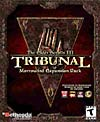
\includegraphics{media/image6.png} for Tribunal functions and

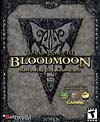
\includegraphics{media/image7.png} for Bloodmoon functions.

To use these functions the respective expansion must be installed (but
not necessarily active). Bloodmoon (and GOTY edition) incorporates all
functions from Tribunal as well.

\hypertarget{working-with-objects}{%
\section{\texorpdfstring{\hfill\break
Working with
objects}{ Working with objects}}\label{working-with-objects}}

\hypertarget{working-with-inventory-items}{%
\subsection{Working with inventory
items}\label{working-with-inventory-items}}

\hypertarget{adding-and-removing-items-from-the-inventory}{%
\subsubsection{Adding and removing items from the
inventory}\label{adding-and-removing-items-from-the-inventory}}

	AddItem, "ObjectID", count\_enum
	
	RemoveItem, "ObjectID", count\_enum

\begin{lstlisting}	
	Actor-> AddItem, "item_ID", 1
	
	Container-> RemoveItem, "itme_ID", 5
\end{lstlisting}

These functions are simple enough, adding or removing items from the
player's or any other inventory, including containers. A
\emph{RemoveItem} call will remove the item from the inventory, it will
"vanish".

\hypertarget{notes-on-additem-by-dinkumthinkum}{%
\subparagraph{Notes on AddItem (by
DinkumThinkum):}\label{notes-on-additem-by-dinkumthinkum}}

If you add items to an NPC's inventory when the inventory screen is
already open, the display won't be updated with the new items, unless
the player manually adds or removes displayed items (which forces the
game to refresh the inventory display).

The early versions of my Potion Saver coded used 'If MenuMode == 1' to
trigger putting potions back into the companion's inventory. This worked
fine when the companion was alive and conscious, since the script would
add the potions while in the dialogue window, \emph{before} the
companion share inventory window was opened.

However, if the companion was dead or unconscious, clicking on the
companion would open the inventory window immediately, and the potions
would be added after the window was already open. End result, the
potions wouldn't show up in the inventory window.\\
\strut \\
To avoid the problem, add items to an NPC's inventory as soon as they
die, as soon as they fall unconscious, or when the game goes into Menu
Mode (check Menu Mode \emph{after} checking death and unconsciousness).
That way, the items will be added before the inventory window opens.\\
\strut \\
Here's the code I used for this in the Potion Saver:

\begin{lstlisting}
	If ( GetHealth < 1 )
	Set DTNPS_HandlePotions to 0
	ElseIf ( GetFatigue < 1 )
	Set DTNPS_HandlePotions to 0
	ElseIf ( MenuMode == 1 )
	Set DTNPS_HandlePotions to 0
	Else
	Set DTNPS_HandlePotions to 1
	EndIf
\end{lstlisting}

\hypertarget{usage-with-containers}{%
\subparagraph{Usage with containers:}\label{usage-with-containers}}

If a container has been emptied by the player (in game), AddItem will no
longer work. One workaround is to replace the container with a new one
each time it's accessed by the player, but this may not be practical as
there's no way to detect when the container is empty. Aragon suggested a
solution:

The workaround is to attach a script to the container that always adds
and removes a dummy item in the same frame that the player activated it.
So, my ingredients chest has a script that looks like:

\begin{lstlisting}
	; Open the chest
	
	Activate
	
	; Always add and remove a dummy (this hack keeps the "AddItem" calls
	working)
	
	AddItem, "misc_de_cloth10", 1
	
	RemoveItem, "misc_de_cloth10", 1
\end{lstlisting}

Furthermore, we make the chest with "references persist". Now we can
reference it from an ingredients sorter using code like:

\begin{lstlisting}
	set count to ( player-> GetItemCount,
	"ingred_dreugh_wax_01" )
	
	while ( count > 0 )
	
	set count to ( count - 1 )
	
	player-> RemoveItem, "ingred_dreugh_wax_01", 1
	
	"_tm_ingredients_chest"-> AddItem,
	"ingred_dreugh_wax_01", 1
	
	endwhile
\end{lstlisting}

Another (probably better) workaround suggested by Enmesharra: Add a
non-carryable light with no world or inventory art associated with it to
the container. It won't show in inventory and thus the container can't
be emptied (not tested).

\hypertarget{notes-on-removeitem}{%
\subparagraph{Notes on RemoveItem:}\label{notes-on-removeitem}}

Removing items that are not present in the inventory does not crash the
game, but the 'RemoveItem' function will subtract the removed item's
weight from the character's encumbrance, EVEN IF the item is NOT in the
character's inventory. So if a script uses 'RemoveItem' to remove a 4
lb. item that the character doesn't have, the character's encumbrance
will wind up 4 lbs. lower than it should be. The workaround for this bug
is to always check for the presence of an item before using 'RemoveItem'
to delete it (Thanks DinkumThinkum for this info).

Don't remove an item that is executing a script, from the item's own
script: that will crash the game. See the example script.

A workaround for this is to use a separate global or local script to
remove the item. However, if the player has \textbf{two or more} copies
of an object with an attached script in their inventory, using
RemoveItem on that Object ID will frequently corrupt data for one of the
remaining copies (you may e.g. see corrupted health or count data).
Equipping or using that corrupt object may cause the game to crash
(Forum info / DinkumThinkum).

To avoid the two known RemoveItem bugs:\\
1. If the object is not scripted, use GetItemCount to be sure the player
has \emph{at least} 1.\\
2. If the object is scripted, use GetItemCount to be sure the player has
\emph{exactly} 1, or make sure the object is unique.

The drop function \emph{does not} have this bug. It does, however, cause
doubling, if used with OnPCEquip / SkipEquip, which can be fixed by
adding and removing any item as described for these functions.

\hypertarget{notes-on-using-additem-removeitem-in-dialogue}{%
\subparagraph{Notes on using Additem / Removeitem in
dialogue:}\label{notes-on-using-additem-removeitem-in-dialogue}}

\textbf{These functions can accept global variables, but only in
dialogue results}, and only if you don't set the global variable in the
same dialog result (Forum info / Argent; According to Argent, the
maximum amount he has been able to add using AddItem, var was 65534
(using a long var=2147483520)). In addition to Argent's info about
AddItem/RemoveItem accepting variables in dialog action boxes: make sure
that the variable in question doesn't change in the same box. Say,
var\_a equals 3 at the moment when the line is selected in dialogue. If
the result field looks like this:

\begin{lstlisting}
	set var_a to var_a + 10 ;
	
	AddItem gold_001, var_a
\end{lstlisting}

three drakes will be added to NPC's inventory, and not thirteen. If such
need arises, put all calculating operators into one dialogue response's
result box, add "choice" operator, and process the AddItem function in
the following response. Also, even with long variables, I couldn't
correctly add values above 32767 (2\^{}15). (tested on pure Morrowind
without expansions) (Forum info / Kir).

Example script:

The following script was discussed on the forums (sorry don't remember
who first made it). It was supposed to ask the player if he wanted to
recycle an item when it was equipped, and then replace that item with
the "recycled" version.

\lstinputlisting{scripts/scr_thing.txt}

It worked nice enough without the \emph{RemoveItem} function in it, but
with that line it would crash. The reason was that this script was
\emph{attached} to item\_a, and thus the running script would be removed
with it, which apparently crashes the game. So the above idea had to be
handled via a global script.

\hypertarget{dropping-items-to-the-floor}{%
\subsubsection{Dropping items to the
floor}\label{dropping-items-to-the-floor}}

	Drop, "ObjectID", count\_enum

\begin{lstlisting}	
	"Actor_ID"-> Drop, "ITEM_ID", 1
\end{lstlisting}

This function is supposed to drop the item from the inventory "to the
calling Actor's feet". This seems to work correctly only for the player
character, dropping the item to his feet. When used on NPC's, the items
are removed correctly from the NPC, but still dropped at the player's
feet.

An interesting note on this is that if they really have that item, they
will drop it, with charges and condition intact. If they don't really
have that item, a new instance will be created. If the player drops an
item he doesn't have, his weight will still be reduced by the weight of
that item - same as the encumbrance bug for RemoveItem (Forum info /
DinkumThinkum).

Note that Drop will only work in active cells: if it is used on an NPC
in an inactive cell, nothing will happen. -(DinkumThinkum)

\textbf{Examples} of use are found in Bethesda's SlaveScript.

\hypertarget{monitoring-inventory-activities-adding-dropping-items-and-using-soul-gems}{%
\subsubsection{Monitoring inventory activities: Adding, dropping items
and using soul
gems}\label{monitoring-inventory-activities-adding-dropping-items-and-using-soul-gems}}

	{[}no fix{]} OnPCAdd (is local short variable)

\begin{lstlisting}	
	Short OnPCAdd
	
	If ( OnPCAdd == 1 )
\end{lstlisting}

This variable is set to 1 when the PC added the object to inventory.
Must be reset manually for multiple use (set OnPCAdd to 0 ).

\textbf{Example:} This is an excerpt from the script attached to
Fargoth's ring, that gives you the magic menu during character creation:

% \textbf{ here
\begin{lstlisting}
	if ( OnPCAdd == 1 ); Player has added the item to the inventory
	
	if ( State == 0 )
	
	EnableMagicMenu
	
	MessageBox "You now have a Magic Menu, where you can see all your
	powers, spells, and magic items." "Ok"
	
	set state to 10
	
	return
	
	endif
	
	endif
\end{lstlisting}
	
{[}no fix{]} OnPCDrop (is local short variable)

\begin{lstlisting}	
	Short OnPCDrop
	
	If ( OnPCDrop == 1 )
\end{lstlisting}

This variable gets set to one when the PC drops the object. Must be
reset manually for multiple use (set OnPCDrop to 0 ).

{[}no fix{]} OnPCSoulGemUse (is local short variable)

\begin{lstlisting}	
	Short OnPCSoulGemUse
	
	If (OnPCSoulGemUse == 1 )
\end{lstlisting}

This gets set to one if the calling Object is a soulgem and it has been
used in either recharging or item making. Must be reset manually for
multiple use (set OnPCSoulGemUse to 0 ).

Example: this is how Azura's star becomes an inexhaustible soulgem:

\lstinputlisting{scripts/AzurasStarScript.txt}

\hypertarget{force-equipping-an-item}{%
\subsubsection{\texorpdfstring{\hfill\break
Force-equipping an Item
}{ Force-equipping an Item }}\label{force-equipping-an-item}}

Equip, "Object\_ID" {[}count\_enum{]}

\begin{lstlisting}
	"Actor_ID"-> Equip, "iron dagger"
\end{lstlisting}

(Also see OnPCEquip function below)

\textbf{Pre-Tribunal: Partly Broken.} This could have been an immensely
useful function. Unfortunately, most of the potential uses do not work:
You can NOT autoequip anything on the Player. You can NOT force the
Actors to equip weapons or armor with this (this is completely governed
by their skills with armor or weapons). You can NOT make "non-removable"
items, like cursed armor, etc. You CAN make Actors swallow potions, or
so I heard.

This Function was \textbf{fixed in Tribunal}. You can now force Actors
to equip armor, weapons and clothing. So you now CAN do all of the above
. Praise to Bethesda.

\textbf{Note}:

The Equip function can make someone equip an item they aren't carrying,
and it will add it to their inventory. However, if you do that then any
scripts on the items won't be run. So you need to use AddItem first,
then Equip, even though Equip does seem to add them. The script will
start if you take the item off the person or out of your inventory and
drop. But while it is in inventories the script doesn't start (Forum
info, ThePal).

In addition, it appears that Equip will only work on the player after at
least one AddItem has been used. -(DinkumThinkum)

The count is optional; if it's omitted then one item will be equipped.
You can't use this to force equip more than one item if it's not
possible to have more than one equipped at a time (e.g. a cuirass) - it
doesn't cause problems but it will still equip only one.

On using equip with variables: it didn't throw any errors, but I got
some strange results. It certainly didn't reliably equip the given
number.

\textbf{Note:\\
}If you equip a potion on a NPC, the NPC will not drink it. You could
get around this by making a spell with the same effects as the potion,
then removing the potion and adding the spell.\textbf{\hfill\break
}

\textbf{Sample Script:} This script (Tribunal required) curses an item
(a Chitin Club) so that it can't be unequipped anymore. Not even using
quick-keys. Bugger! Now you have to fight with a chitin club to the end
of your days, which will probably come soon The player can still use
magic however.

\lstinputlisting{scripts/cursed_item.txt}

\hypertarget{detecting-if-an-item-has-been-equipped}{%
\subsubsection{Detecting if an item has been
equipped}\label{detecting-if-an-item-has-been-equipped}}

{[}no fix{]} OnPCEquip (is local short variable)

\begin{lstlisting}
	Short OnPCEquip
	
	If ( OnPCEquip == 1 )
\end{lstlisting}

The PC has the object equipped (remains true while object is equipped)

This game variable \textbf{(needs to be declared}!) gets set to 1 if the
player is equipping the calling object. It will remain "true" while the
item is still equipped, but gets reset to 0 if the item is unequipped.
So, in some cases you might want to manually reset it:

% \textbf{ here
\begin{lstlisting}
	if ( OnPCEquip == 1 ) ; when the item is equipped
	
	[do something]
	
	set OnPCEquip to 0 ; do this once per equip event...
	
	endif
\end{lstlisting}

The next time the item is unequipped and equipped again, the functions
in {[}do something{]} will be performed again. You can also use a status
variable to control when an effect will be executed. Note that this can
also be processed while in Menu mode:

% \textbf{ here
\begin{lstlisting}
	If ( MenuMode == 1 )
	
	if ( OnPCEquip == 1 ) ; when the item is equipped
	
	[do something]
	
	set OnPCEquip to 0 ; do this once per equip event...
	
	endif
	
	endif
\end{lstlisting}

This script will execute while you are in the menu, as soon as the item
is equipped, while the following will be executed only after you leave
the menu:

% \textbf{ here
\begin{lstlisting}
	If ( MenuMode == 1 )
	
	Return
	
	Endif
	
	if ( OnPCEquip == 1 ) ; when the item is equipped
	
	[do something]
	
	set OnPCEquip to 0 ; do this once per equip event...
	
	endif
\end{lstlisting}

An additional \textbf{Sample Script} can be found above with the Equip
function.

\textbf{Notes:} OnPCEquip was successfully tested with the following item types:

% Itemize?

Clothing

Armor

Weapons

Books/Scrolls (see tips and tricks for correct use, though)

Miscellaneous items

Usable lights

Probes

Potions and Ingredients will only register with OnPCEquip when you use
SkipEquip at the same time, otherwise the item is apparently "destroyed"
before the function registers! Repair objects suffer from this too, and
weirder still, apparatus (or alembics anyway) work the reverse way. They
only seem to trigger OnPCEquip when PCSkipEquip is NOT set (Forum info /
ManaUser).

Apparently books (and maybe some of the other item types that behave
strangely?) set SkipEquip to 1 instead of OnPcEquip! See the tips and
tricks section on this issue.

\hypertarget{disabling-ability-to-equip-an-item}{%
\subsubsection{Disabling ability to equip an
item}\label{disabling-ability-to-equip-an-item}}

{[}no fix{]} PCSkipEquip (is short variable)

\begin{lstlisting}	
	Short PCSkipEquip
	
	Set PcSkipEquip to 1
\end{lstlisting}

Set this to 1 to skip equipping object. Good for popping up messages for
breaking seals on books and such. For an extended example look at the
SealedTreasuryReport script in the editor. Its also great for using e.g.
clothing objects as script triggers in connection with the OnPCEquip
function (see my climbing mod for an example, the climbing gear is
actually a belt, but of course cannot be equipped).

\textbf{Note:} Apparently equipping a book in inventory sets this to one
(instead of setting OnPCEquip to one, as it should). See tips and tricks
section.

There is a bug associated with using this, that leads to duplication of
the item that has the SkipEquip function. I have seen this happen both
with QuickKey usage and when normally equipping items from the inventory
when OnPCEquip is also called. To bypass this, reset the inventory by
adding and removing a dummy item (from within the section of the script
that checks the OnPCEquip function). Do not remove the item with the
script itself, as this causes a crash (see RemoveItem function). If you
have a lot of SkipEquip items, make the item call a global script
(StartScript) that adds and removes the item, e.g.:

\lstinputlisting{scripts/doubling_fix.txt}

\textbf{Sample Script:} Here is a short script I made for a werewolf
mod, it makes an item non-equippable under certain conditions:

\lstinputlisting{scripts/non_equippable.txt}

\hypertarget{checking-for-presence-of-items-in-inventory}{%
\subsubsection{Checking for presence of items in
inventory}\label{checking-for-presence-of-items-in-inventory}}

	GetItemCount, "ObjectID" (returns short)

\begin{lstlisting}	
	Short objectcount
	
	Set objectcount to ( "Mob_ID"-> GetItemCount, "Object_ID" )
	
	If ( GetItemCount, "Object_ID" >= 1 )
\end{lstlisting}

This function checks the inventory of the calling object and returns the
number of objects of type "Object\_ID" it owns.

\hypertarget{section-1}{%
\subsubsection{}\label{section-1}}

\hypertarget{repairing-objects}{%
\subsubsection{Repairing objects}\label{repairing-objects}}

	{[}no fix{]} OnPCRepair (is short variable)

\begin{lstlisting}	
	Short OnPCRepair
	
	If ( OnPCRepair == 1 )
\end{lstlisting}

A game variable that gets set to 1 when the PC repairs the object with
the script. Requires manual reset.

	RepairedOnMe, "Object ID" (returns Boolean/short)

\begin{lstlisting}	
	if ( "daedric_mace"-> RepairedOnMe, "repair_journeyman_01"
	== 1 )
\end{lstlisting}

This function returns 1 if the calling item is repaired by an item of
type "Object ID". Object ID has to be of type "Repair Item" and the
calling object must be either weapon or Armor.

OnRepair

The similar function OnRepair is apparently broken. It should get set to
1 when any repair is attempted at the object: "returns true if calling
object is repaired at all".

\hypertarget{worn-equipped-object-information}{%
\subsubsection{Worn / equipped object
information}\label{worn-equipped-object-information}}

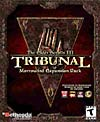
\includegraphics{media/image6.png}

	GetWeaponType (returns short)

\begin{lstlisting}	
	If ( Player-> GetWeaponType == 0 )
	
	;Player uses a short blade
\end{lstlisting}
	
	GetArmorType, armorPart\_enum (returns short, -1 to 2)

\begin{lstlisting}	
	If ( Player-> GetArmorType, 0 == 2 )
	
	;Player wears a heavy helmet
\end{lstlisting}

These functions are called on an Actor to gather information regarding
what the Actor has equipped. GetWeaponType returns the weapon type (see
Table 1.1) of the Actor's current weapon. GetArmorType returns the armor
weight (see Table 1.3) of the Actor's currently equipped armor part. The
armor parts are coded by the numbers listed below (see Table 1.2).
HasItemEquipped returns 1 if the Actor has the given item currently
equipped and 0 if it does not.

Note: If an NPC has a bow but no arrows and fights using hand-to-hand
(no other weapons), GetWeaponType 9 will still return true and
HasItemEquipped will return true for the bow.

\textbf{\hfill\break
Weapon types (Table 1.1):}

\begin{longtable}[]{@{}
  >{\raggedright\arraybackslash}p{(\columnwidth - 2\tabcolsep) * \real{0.61}}
  >{\raggedright\arraybackslash}p{(\columnwidth - 2\tabcolsep) * \real{0.39}}@{}}
\toprule
\endhead
\textbf{Weapon Type Name} & \textbf{Type Number} \\
Unarmed & -1 \\
Short blade, 1 hand & 0 \\
Long blade, 1 hand & 1 \\
Long blade, 2 hand close & 2 \\
Blunt, 1 hand & 3 \\
Blunt, 2 hand close & 4 \\
Blunt, 2 hand wide & 5 \\
Spear, 2 hand wide & 6 \\
Axe, 1 hand & 7 \\
Axe, 2 close & 8 \\
Bow & 9 \\
Crossbow & 10 \\
Thrown weapon & 11 \\
% ? after <
Arrow<?> & 12 \\
Bolt<?> & 13 \\
\bottomrule
\end{longtable}

\textbf{Armor parts (Table 1.2):}

\begin{longtable}[]{@{}
  >{\raggedright\arraybackslash}p{(\columnwidth - 2\tabcolsep) * \real{0.57}}
  >{\raggedright\arraybackslash}p{(\columnwidth - 2\tabcolsep) * \real{0.43}}@{}}
\toprule
\endhead
\textbf{Armor Part Name} & \textbf{Part Number} \\
Helmet & 0 \\
Cuirass & 1 \\
Left Pauldron & 2 \\
Right Pauldron & 3 \\
Greaves & 4 \\
Boots & 5 \\
Left Gauntlet & 6 \\
Right Gauntlet & 7 \\
Shield & 8 \\
Left Bracer & 9 \\
Right Bracer & 10 \\
& \\
\bottomrule
\end{longtable}

\textbf{Armor types / weight (Table 1.3):}

\begin{longtable}[]{@{}
  >{\raggedright\arraybackslash}p{(\columnwidth - 2\tabcolsep) * \real{0.57}}
  >{\raggedright\arraybackslash}p{(\columnwidth - 2\tabcolsep) * \real{0.43}}@{}}
\toprule
\endhead
\textbf{Armor Type Name} & \textbf{Type Number} \\
Unarmored & -1 \\
Light Armor & 0 \\
Medium Armor & 1 \\
Heavy Armor & 2 \\
\bottomrule
\end{longtable}

	HasItemEquipped "item\_ID" (returns short)

\begin{lstlisting}	
	If ( Player-> HasItemEquipped "chitin club" == 1 )
	
	;you poor dolt!
\end{lstlisting}

\textbf{Sample Script:}

When this script is placed on an object, Activating a reference to that
object does ``damage'' to it based on the PC's current weapon and
strength. If the weapon is the specific weapon ``Rock Splitter'' the
object is fully damaged in one hit. When the object is fully damaged, it
explodes sending shards into the PC's face unless he has a shield or a
helmet equipped.

\lstinputlisting{scripts/breakme.txt}

\hypertarget{usedonme-function}{%
\subsubsection{UsedOnMe function}\label{usedonme-function}}

	UsedOnMe, ``Object ID'' (returns Boolean/short)

\begin{lstlisting}	
	if ( UsedOnMe, Misc_pot_redware_01 )
\end{lstlisting}

According to helpfile:

"Returns true if the ``Object ID'' has been used on the calling object.
This is used for scripts that make objects do certain things of the
player uses an object on it."

According to current knowledge this function is broken.

\hypertarget{moving-and-placing-objects}{%
\subsection{Moving and placing
objects}\label{moving-and-placing-objects}}

The following functions do not work on the player, NPCs or monsters.
They do work on static objects, activators, containers, miscellaneous
objects etc. \textbf{Note:} Actors, including the PC tend to fall
through moving objects after a while. This can be avoided by quickly
disabling and enabling a moving object every frame -- doing this
apparently updates the collision information. Actors can also be
equipped with a levitate or slowfall ability to further decrease the
chance of falling through objects (for more details see the tips and
tricks section on ridable objects by MadMax).

\hypertarget{moving-along-an-objects-axis}{%
\subsubsection{Moving along an objects
axis}\label{moving-along-an-objects-axis}}

	Move axis(x/y/z), units/sec\_enum

\begin{lstlisting}	
	Move x, 100
	
	Object_ID-> Move Z, 30
\end{lstlisting}

Moves the object along the selected axis (x, y, or z) at the speed
selected. This speed is in units per second (21.3 units per foot). Thus,
the distance moved per frame will depend on your frames per second,
while the distance moved in a unit time will not. This movement is based
on the object's local coordinate system. Thus, a positive y movement
will always move the object along its local forward vector:

% Missing math image.

\textbf{Note:} Move will not work on Actors, including the player.
However, it will work on dead actors (Forum info / Argent). As with all
functions using a "fix", move requires that the object is placed into
the game world in the editor, before you can use it in a script:

\begin{lstlisting}
	PlaceAtPC "My_Object", 1,1,1
	
	My_Object-> Move x, 10
\end{lstlisting}

will not work if "My Object" has not already been placed, but you can
have a local script running on "MyObject" that just uses

\begin{lstlisting}
	Move x, 10
\end{lstlisting}

\hypertarget{moving-along-the-world-axis}{%
\subsubsection{Moving along the world
axis}\label{moving-along-the-world-axis}}

	MoveWorld axis(x/y/z), units/sec\_enum

\begin{lstlisting}	
	MoveWorld z, 100
	
	Object_ID-> MoveWorld Z, 30
\end{lstlisting}

Moves the object along the selected world axis (x, y, or z) at the speed
selected. This speed is in units per second (21.3 units per foot). This
movement is based on the world axis, thus a positive z movement will
always move the object up, regardless of its local rotation: In world
coordinates Z is always up / down (increasing upwards), X is east / west
(increasing to east) and Y is north / south (increasing to north).

% Missing math image.

\textbf{Note:} MoveWorld will not work on Actors, including the player.
Use SetPos for actors.

This is an \textbf{example} after a script I once picked up on the
forums that makes a platform slowly move out and back once the player
stands on it:

\lstinputlisting{scripts/platform_script.txt}

\hypertarget{cellupdate}{%
\subsubsection{CellUpdate}\label{cellupdate}}

CellUpdate

\textbf{Broken!} According to Bethesda: Updates the current object's
cell position. This should be called when moving objects over large
distances. The game keeps tracks of objects based on what cell they are
in, and if an object moves a cell over from its starting position, it
may not get processed correctly when running its script.

The part about not processing correctly is certainly right. Objects can
disappear or "warp" if moved too far from the place they were created
in. Unfortunately my attempts to use this function always resulted in a
runtime error: "need to add function code for function CellUpdate".

\textbf{Note:} a way around this problem (requires Tribunal) is to
disable and delete (SetDelete) the object on a regular basis (for
ridable objects upon entering a new cell) and immediately placing a new
version (PlaceItem) at the very same position using a global script
(seen in MadMax boat script from the Fishing Academy Mod). See the Tips
and Tricks section for an in-depth explanation by MadMax himself. This
works like a charm, because this way the object never really leaves the
cell it was created in.

\hypertarget{setting-position-the-other-way-to-do-movement}{%
\subsubsection{Setting position (the other way to do
movement)}\label{setting-position-the-other-way-to-do-movement}}

SetPos, axis, float\_enum\_pos (float\_var with Tribunal/Bloodmoon)

\begin{lstlisting}	
	SetPos, z, 477
	
	Object_ID-> SetPos X, 466
\end{lstlisting}

This function (unlike the move and moveworld functions) also works with
Actors, including the player. Axis is x, y, or z. The float value sets
the position of the calling object to that value. This always refers to
the local coordinate system the object is currently in.

\textbf{Note:} With Tribunal, this function accepts local float
variables, but only within the currently active cells. This is relevant
for exteriors, you can not move objects an arbitrary distance, the
target location must be within the active cells (current cell of player
plus surrounding cells). (Forum info / reposted by Srikandi). Also note
that while objects can be SetPos to any position (without collision
being detected), Actors will still check for collision, and may not move
as expected in case of collision (which can be used to good effect for
collision detection).

\textbf{SampleScript:} This script is made for floating crates in the
Mournhold sewer (Tribunal). It demonstrates how \emph{SetPos} and
\emph{SetAngle} can be used instead of \emph{MoveWorld} and
\emph{Rotate} to produce fluid movements:

\lstinputlisting{scripts/floatAboveStartHeight.txt}

\hypertarget{positioning-an-object-in-the-world-or-in-an-interior-cell}{%
\subsubsection{Positioning an object in the world or in an interior
cell}\label{positioning-an-object-in-the-world-or-in-an-interior-cell}}

	\textbf{Position, float\_enum\_x, float\_enum\_y, float\_enum\_z,
		float\_enum\_zRot}

(for outdoors)(floats accepted with expansions)

	\textbf{PositionCell, float\_enum\_x, float\_enum\_y, float\_enum\_z,
		float\_enum\_zRot, ``cellID''\\
	}(for interior / exterior cells) (floats accepted with expansions)


\begin{lstlisting}	
	position -23515, -15355, 3355, 90
	
	Player-> position -23515, -15355, 3355, 90
	
	"Actor_ID"-> PositionCell, -254, 475, -376, 360, "Balmora,
	Council Club"
\end{lstlisting}

The classic application for this function is the teleport ring,
transporting the player to certain locations. However, it can also be
used to warp NPCs or objects to a new location. Note that in original
Morrowind this function only accepted literal values as arguments. (This
probably changed with Tribunal: not sure if in all versions or only with
the expansions, but: Position/PositionCell can take float variables, but
they must be LOCAL variables! (info by Indigo Rage).

Z\_Rot is not set in degrees (0-360°) but in minutes (1° = 60 min): So,
if you want the person to face east, use 5400. South, 10800. West 16200.

However, for some reason degrees are used for the player (thanks to Axel
for pointing this out).

\textbf{Notes:}

Using PositionCell in dialog results isn't reliable, and may cause
crashes: some users have no problems with it, but for others it will
crash the game, and for some users it may simply fail unpredictably
(this doesn't seem to be version-dependent, not sure what causes it).
The way Bethesda does this correctly is to use StartScript to start a
script that does the teleporting. (Forum Info/Emma).

You should not use this function on items that are in the players
inventory, this causes MW to crash (Forum info/Nigedo).

If you are repositioning the player immediately on detecting PC cell or
CellChanged (e.g. preventing teleport to a forbidden destination), you
may need to introduce a delay of one or two frames before using
PositionCell to move the player back out of the cell, otherwise the
player may not end up at the correct coordinates. (Forum info /
Monica21)

\textbf{Sample Script:} A simple teleport ring could look like this:

\lstinputlisting{scripts/TeleportScript.txt}

Note that both targets are outdoor cells and the different formats used.
If you try to teleport to an unsafe place (clipping with an object or
out in the void), you will instead be placed at the next safe location.

Sometimes the PositionCell format given above won't work (even though it
should): If there are no errors but nothing happens, try replacing, e.g.

\begin{lstlisting}
	Player-> PositionCell -21278, -17613, 534, 0, "Balmora (-3,
	-3)"
\end{lstlisting}

with

\begin{lstlisting}
	Player-> PositionCell -21278, -17613, 534, 0, "Balmora"
\end{lstlisting}

I've found that sometimes one method works and sometimes the other.

\hypertarget{resetting-an-object-to-its-original-position}{%
\subsubsection{Resetting an object to its original
position}\label{resetting-an-object-to-its-original-position}}

SetAtStart

\begin{lstlisting}
	SetAtStart
	
	Object_ID-> SetAtStart
\end{lstlisting}

This resets the object to the original position it was given in the
editor, before any movement or rotation occurred. For an example, see
the moving platform script example under the topic "moving along the
world axis". See the \emph{Move} function for a sample script.

\hypertarget{placing-an-item-near-the-pc}{%
\subsubsection{Placing an item near the
PC}\label{placing-an-item-near-the-pc}}

{[}no fix{]} PlaceAtPC, "Object\_ID", count\_enum, distance\_enum,
direction\_enum

\begin{lstlisting}
	PlaceAtPC, "Secret Message", 0, 30, 1
	
	PlaceAtPC, "ancestor_ghost", 1, 256, 1
\end{lstlisting}

This function places a new reference of "Object\_ID" near the player.
The function lets you define a direction relative to the player where
the object is going to appear and a distance (in units). If that
location is not safe (in the air, in a wall, etc), the object will be
placed at one of the other axis or at the player's exact location
(feet). (Erratum: Thanks to Isildur and Esteban for pointing out that
number\_enum and distance\_enum were switched around in previous
versions.)

Direction is:

0 = front

1 = back

2 = left

3 = right

Note (DinkumThinkum):

\emph{According to Bethesda, on the PC version an overflow loot bag will
be created if there are more than 1024 objects in a single cell.}

\emph{\hfill\break
However, if you try to put a large number of objects into a cell using
'PlaceAtPC', the game will lockup completely. Don't know the minimum
number that will cause the crash, but 'PlaceAtPC p\_restore\_health\_e
2000 0 0' will definitely do it.}%☺

In other words: the game engine won't create an overflow loot bag for
excess items that are added to a cell by a script; instead, it just
crashes when the maximum number of items per cell is exceeded. I ran
into this with 'PlaceAtPC', but I would guess that any script function
that adds items to a cell would have the same problem. I would also
guess that the crash occurs as soon as the number of items in the cell
reaches the number that would normally trigger the creation of an
overflow loot bag.

\hypertarget{place-items-near-an-object}{%
\subsubsection{Place items near an
object}\label{place-items-near-an-object}}

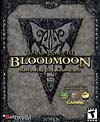
\includegraphics{media/image7.png}

PlaceAtMe "Item\_ID" count\_enum, distance\_enum, direction\_enum

\begin{lstlisting}
	Object-> PlaceAtMe `Item_ID' count_enum distance_enum
	direction_enum
\end{lstlisting}

The PlaceAtMe function works the same as PlaceAtPC without it being
centered on the PC. Bloodmoon uses this to place attackers in different
places depending on the player's distance at the time. This allows the
script to make it appear as though there is a large number of opponents
that just keep coming, among other things.

% \textbf{ here
\begin{lstlisting}
	;THIS POPS IN A HUNTER AT APPROPRIATE SPOT, INCREMENTS HUNTERCOUNT, AND
	RESETS TIMER
	
	if ( popA == 1 )
	
	"active_BM_hunter1"-> PlaceAtMe skaal_hunter 1 1
	1
	
	set huntercount to ( huntercount + 1 )
	
	set timer to 0
	
	elseif ( popB == 1 )
	
	"active_BM_hunter2"-> PlaceAtMe skaal_hunter 1 1
	1
	
	set huntercount to ( huntercount + 1 )
	
	set timer to 0
	
	elseif ( popC == 1 )
	
	"active_BM_hunter3"-> PlaceAtMe skaal_hunter 1 1
	1
	
	set huntercount to ( huntercount + 1 )
	
	set timer to 0
	
	endif
\end{lstlisting}

\hypertarget{creating-new-object-references-with-placeitem}{%
\subsubsection{Creating new object-references with
PlaceItem}\label{creating-new-object-references-with-placeitem}}

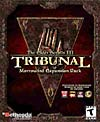
\includegraphics{media/image6.png}

{[}no fix{]} PlaceItem "object ID", float\_var\_X, float\_Y, float\_Z,
float\_Zrot

{[}no fix{]} PlaceItemCell "object ID", "cellID", X, Y, Z, Zrot

% Degree symbol here. °

These functions are used to create new references to objects. PlaceItem
will create a reference to object "Object ID" at coordinate (X, Y, Z)
with Z rotation Zrot in the current cell. \textbf{Z\_Rot is not set in
degrees (0-360°) but in minutes (1° = 60 min): So, if you want the
person to face east, use 5400. South, 10800. West 16200.}

The function accepts (local) float variables. PlaceItemCell does the
same thing as PlaceItem except it allows you to specify a cell other
than the current one in which the object should be created. With either
function, if the target cell for the reference is an exterior cell and
the given coordinate is outside of that cell, then the reference will be
added to the cell containing the coordinate. This is a nice addition
that allows you to add things to the world without previously placing
them in the editor.

JOG posted the following interesting info on PlaceItemCell:

Well, When I first tried PlaceitemCell, I thought it's a great function
to place items instead of having a "storage-cell" where the objects lie
around until the game needs them. I soon realized that you can't refer
to those objects by script. (To disable them for example.) The script
won't compile until at least one of the objects is in use, and then the
disable command would refer to that object, so you still need
PositionCell.

(Note by GBG: you can circumvent this for many applications by having a
script on the placed item, so that you can omit the "fix" and have
functions such as disable reference to it by default.)

DinkumThinkum adds:

PlaceItemCell would have been perfect for what I wanted to do, until I
discovered that the placed NPC disappeared if I saved and reloaded
before going to the cell they were placed in.

(Note by GBG: This can be avoided in most cases by making the placing of
the NPC conditional on the player entering the cell. I still think
PlaceItem is a very useful function.)

Sample Script:

Putting this script on an object causes it, on activation, to ask the
user for an object type and then to create a reference to the specified
object at 100 units above the activated reference with 45 degree Z
rotation. If the key is selected, it is created at that same coordinate
and rotation in the cell ``key room'' rather than the current cell.

\lstinputlisting{scripts/makethingsimple.txt}

\hypertarget{rotation-and-angles}{%
\subsection{\texorpdfstring{Rotation and angles
}{Rotation and angles }}\label{rotation-and-angles}}

Bethesda uses both degrees and minutes (1° degree = 60 minutes) as units in scripting functions:

	GetAngle {[}\textdegree{]} (-180 to 180 \textdegree)\\
	Setangle {[}\textdegree{]}\\
	Position {[} min \textdegree{]}\\
	PositionCell {[}min{]} \emph{except for the player {[}\textdegree{]}}\\
	PlaceItem {[}min{]}\\
	PlaceItemCell {[}min{]}\\
	Rotate {[} \textdegree / second {]}\\
	RotateWorld {[} \textdegree / second {]}

\hypertarget{making-an-object-spin}{%
\subsubsection{Making an object spin}\label{making-an-object-spin}}

Similar to the movements described above, you can also rotate objects,
around either their local or the world axis and determine the current
angle:

% Degree symbols not working in listings environment.

	Rotate , axis, angle/sec\_enum
	
	RotateWorld, axis, angle/sec\_enum

\begin{lstlisting}	
	Rotate, z, -30; rotate counterclockwise, 30 per second, around objects
	z axis
	
	Object_ID-> Rotate, Y, 100
\end{lstlisting}

Axis can be x, y, or z. Notice that like the move functions the value
you are giving Rotate or RotateWorld is a speed setting (not an angle),
if you want to turn an object by 90\% either use set angle (for an
instantaneous change) or use Rotate together with GetAngle to check how
far the object has already been turned. These functions can not be used
with Actors.

RotateWorld does NOT update an item's position.\\
If you use RotateWorld in a script, and then call GetAngle, it will
always return the same value, regardless of what the angle actually is.
Just using rotate does not cause this problem.

(Forum info / HeyYou)

\hypertarget{setting-angles}{%
\subsubsection{\texorpdfstring{Setting Angles
}{Setting Angles }}\label{setting-angles}}

SetAngle, axis, float\_enum\_angle

\begin{lstlisting}
	SetAngle, z, 30
	
	Object_ID-> Setangle, z, 25
\end{lstlisting}

This function sets the object to a specific world angle. Axis is x, y,
or z. The float value sets the angle (in degrees) of the calling object
to that value. This always refers to the local coordinate system the
object is currently in.

\textbf{Note:} According to console test, this does not affect Actors.
With Tribunal, this function accepts local float variables, but only
within the currently active cells. This is relevant for exteriors, you
can not move objects an arbitrary distance, the target location must be
within the active cells (current cell of player plus surrounding cells).
(Forum info / reposted by Srikandi). For actors, see the "Face, x, y"
function.

Notes (by Simpleton):

SetAngle doesn't work how sfd says it does. My guess is nobody ever
noticed before because nobody ever uses it with the X or Y axis, which
is where it gets funky. I wasn't going to explain how it worked because
it's long and complicated and nobody but me cares, but I've got time to
kill and there's always a chance somebody will run across this problem
and need help.\\
\strut \\
Probably the oddest thing about SetAngle, X/Y is that neither have
anything to do with the X or Y axis'. Luckily they do have a system to
them that, with a bit of imagination, isn't too hard to understand. The
way I found easiest to understand was to imagine a protractor with an
arm being held up at a bit of an angle, so that flat side is on the
table and the curved part is about 45 degrees off the table. The angle
between the table and the protractor is y, and the angle of the arm on
the protractor is x.\\
\strut \\
There are a couple differences, one being that if you set y to 0 the
"protractor" is pointing straight up, and a positive x actually goes
down instead of up (i.e. the "arm" would go down into the table). So if
you set all the angles to 0 and then add 1 to x each frame the object
would spin in a vertical circle that is moving down while it's pointing
at you. But, if y is 90 (protractor is lying flat on the table) then
adding 1 to x each frame would spin the object around the z axis.\\
\strut \\
Interestingly in the last example if you were to add 1 to *z* each frame
you would get the same results. That's because while what changing x
does depends on the angle in y and vise versa, changing z always does
the same thing: spin the object around the z axis.\\
\strut \\
So, there ya go, and even if you don't understand what I said, you have
to give me credit for pulling that picture of a protractor out of my
a**.

(ManaUser:)

I'm afraid I don't understand the protractor analogy but the worst thing
about SetAngle is that it doesn't always save right. Particularly when
an object has been rotated on more than one axis, I've noticed it facing
some wonky direction after reloading.

\textbf{Example script: See SetPos function}

\hypertarget{scale-functions}{%
\subsection{\texorpdfstring{\hfill\break
Scale Functions}{ Scale Functions}}\label{scale-functions}}

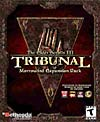
\includegraphics{media/image6.png}

	GetScale (float)
	
	SetScale newScale\_float
	
	ModScale scaleChange\_float

\begin{lstlisting}	
	If ( doonce == 0 )
	
	Object_ID-> SetScale 0.1
	
	Set doonce to 1
	
	endif
\end{lstlisting}

These functions are used to determine or modify the scale of a
reference. Any scale you can set must be within (exclusively) 0 and 10
(so you can set it beyond 0.5 and 2, contrary to what was written in the
original description by Bethesda) (info by Mode Locrian). The above
sample script can thus be used to set scale beyond the limits of what
the TES CS itself allows.

\textbf{Notes:} You shouldn't call "setscale" in every frame, at least
not in exteriors or other FPS-critical situations.

The scale will be reset to a value within the 0.5 - 2.0 frame when you
reload. So don't use a done-flag to call it only once. Either call it
regularly (about all 10 frames) or test for "getscale" and reset the
scale when it doesn't fit:

\begin{lstlisting}
	if ( GetScale != 5 )
	SetScale, 5
	endif
\end{lstlisting}

Another way is to set it in a Tribunal or Bloodmoon start script. This
can be done once, and will make sure the scale is set each time you load
a game. (Forum info / JOG).

Sample script:

A more complex sample script by Bethesda shows how to grow and shrink an
object.

When this script is placed on a reference, activating that reference
gives the user the ability to change that reference's scale.

\lstinputlisting{scripts/scalescript.txt}

\hypertarget{determining-location-relative-position-and-movement}{%
\subsection{\texorpdfstring{\hfill\break
Determining location, relative position and
movement}{ Determining location, relative position and movement}}\label{determining-location-relative-position-and-movement}}

\hypertarget{detecting-if-player-is-indoors-or-outdoors}{%
\subsubsection{Detecting if player is indoors or
outdoors}\label{detecting-if-player-is-indoors-or-outdoors}}

{[}no fix{]} GetInterior (returns Boolean/short)

\begin{lstlisting}
	If ( GetInterior == 1 )
\end{lstlisting}

\textbf{Undocumented function!} (Thanks XP-Cagey and Killgore)

This function will return 1 if the current cell is an interior cell and
0 if it is an exterior cell. It will also return 1 if the player is in
an interior acting like exterior (GetWindSpeed can be used to detect a
fake exterior).

The following is a global sample script by Killgore. If you want to try
it out start it by typing "StartScript Outside\_Check" in the console.

\lstinputlisting{scripts/Outside_Check.txt}

\hypertarget{determining-the-players-cell}{%
\subsubsection{Determining the players
cell}\label{determining-the-players-cell}}

{[}no fix{]} GetPCCell, "Cell\_ID" (returns Boolean/short)

\begin{lstlisting}
	if ( GetPCCell "Balmora" == 1 )
	
	Set dream to 1
	
	endif
\end{lstlisting}

The GetPCCell function tests for the player's presence in the specified
cell. It returns 1 if the player is in the specified cell, 0 if not.
Partial matches are supported, e.g. GetPCCell, "Vivec" will return true
for the cells "Vivec", "Vivec, foreign quarter waistworks" and "Vivec,
temple", etc.

Sample Script:

This small Bethesda script checks for the PC leaving a certain area
until removing a certain item from an NPC:

\lstinputlisting{scripts/DrothPost.txt}

\hypertarget{distance-of-one-object-to-another}{%
\subsubsection{Distance of one object to
another}\label{distance-of-one-object-to-another}}

GetDistance, "ObjectID" (returns float)

\begin{lstlisting}
	"ObjectID1"-> GetDistance, "ObjectID2"
\end{lstlisting}

This function returns the distance (in units) of one object to another.
In syntax one, that is the distance between the calling object (to which
script is attached to) and the named object. This can be used to trigger
attacks or other events, or simply to roughly determine the player's
whereabouts for use in a script.

Here is a snippet from an original Morrowind script:

% \textbf{ here
\begin{lstlisting}
	; From a script attached to an NPC Ashamanu:
	
	; Ashamanu will give journal entry 60 when player is near
	
	if ( GetDisabled != 1 )
	
	if ( GetDistance Player <= 256 )
	
	if ( GetDistance "guar_white_unique" <= 256 )
	
	if ( GetJournalIndex "MS_WhiteGuar" <= 50 )
	
	Journal "MS_WhiteGuar" 60
	
	endif
	
	endif
	
	endif
	
	endif
\end{lstlisting}

Limitations:

\begin{itemize}
\item
  GetDistance requires that the object given as parameter is placed in
  the gameworld (in the editor) and has references persist checked (or
  is naturally persistent such as an NPC).
\item
  Note that you should use this function only with unique ID's or in
  environments where you exactly know that there is only one instance of
  the ID -- otherwise the Game engine will just grab the first instance
  of the ID it finds and report that distance -- most likely not the
  distance to the object you want. Thus, a script that warns the player
  of the presence of a slaughterfish that is closer than 800 units would
  have to be attached to the ID of the slaughterfish, and check the
  distance to "player" (which is unique), not vice versa.
\item
  If you determine distance to an object you are moving with Move or
  MoveWorld, GetDistance will still report the \textbf{distance to the
  original location} of the object (the one you set in the editor). Use
  GetPos and good ol' Pythagoras (c\textsuperscript{2} =
  a\textsuperscript{2} + b\textsuperscript{2}) to determine distances in
  these instances.
\item
  GetDistance won't work on disabled objects.
\end{itemize}

\hypertarget{determining-an-objects-position-and-facing}{%
\subsubsection{Determining an objects position and
facing}\label{determining-an-objects-position-and-facing}}

GetPos, axis(x/y/z)

\begin{lstlisting}
	Object_ID-> GetPos, z
\end{lstlisting}

When you are moving objects with the Move/MoveWorld functions described
above, you might want to obtain information on its current whereabouts.
This functions work on Actors and objects. In the following sample
script I used this function to control the movement of a light source (a
fire) to make a fire pit where the flames actually start slowly and die
down in the evening on a daily schedule -- the fire objects original Z
position is 511:

\lstinputlisting{scripts/_HB_Scheduled fire.txt}

GetAngle , axis(x/y/z) (returns float)

\begin{lstlisting}
	If ( Object_Id-> GetAngle, z == 180 )
\end{lstlisting}

The GetAngle function returns the world angle, not the local angle.
World angles are from 0 to 180 and 0 to -180 (see figure for z axis).

\textbf{Note:} This works on actors and objects, however for the player
(and I assume other actors) only the z axis is relevant - GetAngle, x or
y always return 0.

% Missing math image here.

\hypertarget{line-of-sight}{%
\subsubsection{Line of Sight}\label{line-of-sight}}

GetLOS, ObjectID (returns Boolean/short)

\begin{lstlisting}
	Actor_ID-> GetLOS, Player
\end{lstlisting}

Undocumented:

GetLineOfSight (returns Boolean/short)

These functions determines whether the calling object has line-of-sight
to the referenced object. It does not seem to work for non-Actor type
objects, as far as I could determine. It does not take facing into
account, so don't take the "sight" part too literally. (See "Is she
looking at me?" in the Tips and Tricks section.)

\textbf{Note}: GetLOS is a very slow function, don't let the script call
it every frame.

\textbf{Sample Script}:

\lstinputlisting{scripts/balynScript.txt}

\hypertarget{section-2}{%
\subsubsection{}\label{section-2}}

\textbf{Note:}

getLOS and getLineOfSight suffer from the same problem with generic NPCs
as getDetected (see below)\\
% link?
\protect\hypertarget{_Toc182634542}{}{}\emph{\textbf{Determine whether
an Actor is detected by another Actor}}

{[}no fix{]} GetDetected, "Actor ID" (returns Boolean/short)

\begin{lstlisting}
	If ( GetDetected, Player == 1 )
\end{lstlisting}

Returns true if \textbf{any} calling Actor can detect "Actor ID" (thanks
for the correction, ThePal!). This function will return 0 if the Actor
is hidden in some form, e.g. is sneaking successfully, or has an
invisibility or chameleon spell active. According to the helpfile this
is a slow function, do not call it a lot (e.g. make a counter to only
call it every 3 seconds).

\textbf{Sample script:} The player must approach an object undetected --
if not he is "caught"

\lstinputlisting{scripts/jeanneScript.txt}

GetDetected calling an NPC's ID if there's more than one reference in
the game will return nothing. For example:

\begin{lstlisting}
	getDetected, "fargoth"
\end{lstlisting}

will return 1, but:

\begin{lstlisting}
	GetDetected "Imperial Guard"
\end{lstlisting}

Returns nothing. (Not 0, it doesn't return a value). However if you
reference an exact NPC:

\begin{lstlisting}
	GetDetected "Imperial Guard00000002"
\end{lstlisting}

A value is returned.

(Forum info / Fliggerty )

\hypertarget{determining-when-the-pc-leaves-a-cell}{%
\subsubsection{Determining when the PC leaves a
cell}\label{determining-when-the-pc-leaves-a-cell}}

{[}no fix{]} CellChanged

\begin{lstlisting}
	If ( CellChanged == 1 )
\end{lstlisting}

CellChanged returns 1 for one frame when player changes cells. It
doesn't return 1 for scripted teleporting or magic teleporting.
CellChanged returns true almost immediately after the player changes
cells. This means a local script running in an interior cell won't fire
when the user leaves a cell, but rather when the player enters the cell.

Scripted teleporting may trigger CellChanged if the script is global or
targeted (local scripts will not trigger it). (Forum info / Zennorious,
Tamandra)

Note:

CellChanged doesn't always trigger, even if the player enters the cell
via a normal teleport door. Possibly scripts running in the cell can
have some effect on this, somehow. ForceGreeting seems to muck it up in
particular (and no there wasn't a menumode return in that script).

\textbf{Sample Script:} In the SlaveScript, which governs freeing slaves
in the game, CellChanged is the trigger to disable the slave -- the
slave has left for a better future:

\lstinputlisting{scripts/SlaveScript.txt}

another nice example is the Gateway Haunt's script. This spectre always
comes back just when you are not watching:

\lstinputlisting{scripts/ResurrectHaunt.txt}

\hypertarget{detect-player-traveling}{%
\subsubsection{Detect player traveling}\label{detect-player-traveling}}

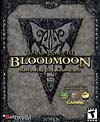
\includegraphics{media/image7.png}

{[}no fix{]} GetPCTraveling (returns boolean)

\begin{lstlisting}
	if ( GetPCTraveling == 1 )
\end{lstlisting}

Bloodmoon adds a functions to check whether the PC is traveling (i.e. on
a Silt Strider). Will return 1 if traveling/in jail, zero otherwise.
This is used in the werewolf change script to stop the PC from changing
if either of these are true:

\begin{lstlisting}
	if ( PCWerewolf != 1 ) ; DON' RUN IF PLAYER ISN'T WEREWOLF
	
	return
	
	endif
	
	if ( \textbf{GetPCinJail} == 1 )
	
	return
	
	endif
	
	if ( \textbf{GetPCTraveling} == 1 )
	
	return
	
	endif
\end{lstlisting}

\hypertarget{triggers-for-actors-standing-on-an-object}{%
\subsubsection{Triggers for Actors standing on an
object}\label{triggers-for-actors-standing-on-an-object}}

GetStandingPC (returns Boolean/short)

returns 1 if PC is standing on it.

GetStandingActor (returns Boolean/short)

returns 1 if ANY Actor (including PC) is standing on it.

\begin{lstlisting}
	If ( Object_Id-> GetStandingPC == 1)
	
	[... trigger horrible trap]
	
	endif
\end{lstlisting}

These are great functions to trigger events, especially for interior
cells. It is also an excellent function to build traps. You can make an
"activator" object using the nif files of any static object (hallway,
carpets etc.), and trigger certain events once the player (or another
Actor) steps on that object.

My sample script is used to light fires in a hall on as soon as the
player steps on a particular piece of floor:

\lstinputlisting{scripts/HBHallLighting.txt}

HB\_hallfire is a global variable, used to turn on the fire. This is the
script for the fire:

\lstinputlisting{scripts/HBHallfireon.txt}

\hypertarget{hurting-an-actor-standing-on-an-object}{%
\subsubsection{Hurting an Actor standing on an
object}\label{hurting-an-actor-standing-on-an-object}}

HurtStandingActor, float\_HP/s

\begin{lstlisting}
	HurtStandingActor -3
	
	Object_ID-> HurtStandingActor 1
	
	Float hurt_variable
	
	HurtStandingActor, hurt_variable
\end{lstlisting}

This function affects the health of an Actor (including the PC) that
stands on the object. Positive values will reduce health, negative
values heal (hitpoints per second). Using negative values will modify
your health even beyond your normal maximum health, so be careful to
test this if you want to use this function this way. This function
accepts float variables.

\textbf{Sample script:} The effect is probably best known from the lava
fields:

\lstinputlisting{scripts/lava01.txt}

\hypertarget{object-collision-functions}{%
\subsubsection{Object Collision
Functions}\label{object-collision-functions}}

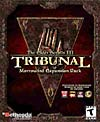
\includegraphics{media/image6.png}

GetCollidingPC (returns Boolean/short)

GetCollidingActor (returns Boolean/short)

\begin{lstlisting}
	if ( GetCollidingPC == 1 )
\end{lstlisting}

HurtCollidingActor, damage\_enum

\begin{lstlisting}
	HurtCollidingActor, 100
	
	Object_ID-> HurtCollidingActor, 100
\end{lstlisting}

These functions go on an object to allow it to interact with Actors
colliding with it. GetCollidingPC returns 1 if the PC is currently
colliding with the object and 0 otherwise. GetCollidingActor works the
same as the PC version of the function but will return 1 if any Actor
(other than the PC) is colliding with the object. HurtCollidingActor
lowers the colliding Actor's health Damage points every second.

\textbf{Note:} An object has to have collision to trigger these
functions, so if you can walk through the object, none of these
functions will trigger.

Sample script:

When this script is placed on an object, any Actor touching that object
will take damage. A different message is given depending on whether the
Actor is the PC or someone else.

\lstinputlisting{scripts/hurtActor.txt}

\hypertarget{section-3}{%
\subsection{}\label{section-3}}

\hypertarget{section-4}{%
\subsection{}\label{section-4}}

\hypertarget{checking-activation-of-an-item-and-activating-it}{%
\subsection{Checking activation of an item and activating
it}\label{checking-activation-of-an-item-and-activating-it}}

An item is usually activated when you press the spacebar to "use" it.
Most items have a standard action that is performed when they are
activated: Doors open, chests display their content, Actors initiate
dialogue etc. The OnActivate function allows you to intercept the
standard action and do something else or check a condition first:

OnActivate
\begin{lstlisting}
	If ( OnActivate == 1 )
\end{lstlisting}

This get set to one for one frame when the object is activated.
OnActivate resets itself as soon as the function is called, so only one
script can report OnActivate successfully, and you should only have one
OnActivate call in your script at each moment. OnActivate short-circuits
the normal behavior of the object -to perform the standard action of the
object once OnActivate has been called, you have to use the activate
command:

Activate

\begin{lstlisting}
	activate (if script is on the object to activate)
\end{lstlisting}

Activate can be used to trigger the standard action of an object, after
OnActivate has been called.

\textbf{Standard actions called by Activate are:}

Doors -> Open (Possibly broken in Original MW, with
v1.6.1820 it definitely works).

LoadDoors -> Open (If used with OnActivate)

Containers -> Open (show contents)

Books/scrolls -> Display text to read.

Activators -> Nothing

Actors -> Dialogue

Weapon -> Pick up

Armor -> Pick up

Miscellaneous -> Pick up

Not tested, but I assume:

Equip. Lights -> Pick up

Other Lights -> Nothing

Probes -> Pick up

Apparatus -> Pick up

Example script:

The following script demonstrates the use of OnActivate nicely. It is
attached to a container object, a chest that does NOT advertise its trap
like the normal in-game ones do:

\lstinputlisting{scripts/Trap_script.txt}

\textbf{Notes}: According to my testing, the activate function can not be used by itself, without OnActivate in the same script. The OnActivate and Activate functions can be in different parts of the script, though. However, Activate will not work before OnActivate has not at least been called once. There have been reports that the object also must have been manually activated at least once within the last 72 hours, so apparently the game eventually forgets that OnActivate has been called previously. Containers require manual activation each load session (forum info / Phaedrus). Play around with this testscript (I had it attached to a door) to
see for yourself:

\lstinputlisting{scripts/GBG_closing_door.txt}

There have also been various reports about difficulties with on
OnActivate in general, in my experience, avoiding to use more than one
OnActivate in a script is the safest way to go. Also be aware that for
items in your inventory, OnPCEquip may be the function to use instead of
OnActivate, as OnActivate does not get called by moving the item over
the Player icon.

Info from the UESP: There is an undocumented feature in the Activate
function by specifying the player after the function, for example:

\lstinputlisting{scripts/RemoteContainer.txt}

If the container is persistent (references persist) this script should
open the container wherever the player is. This is a great way to create
'carryable' containers by attaching a script similar to the above to a
ring or similar item.

\hypertarget{locking-and-unlocking-doors-or-chests}{%
\subsection{\texorpdfstring{\hfill\break
Locking and Unlocking doors or
chests}{ Locking and Unlocking doors or chests}}\label{locking-and-unlocking-doors-or-chests}}

Lock, short\_enum\_locklevel

Unlock

\begin{lstlisting}
	My_Door-> Lock, 50
\end{lstlisting}

GetLocked (returns Boolean/short)

\begin{lstlisting}
If ( GetLocked == 1 )

Unlock

Endif
\end{lstlisting}

(only Door and container objects)

These functions are used to lock and unlock doors or containers. The
GetLocked function returns 1 when the calling object is locked. Lock
locks the object with the lock level specified (0-100). Lock 0 has an
odd effect though. The door/container will be neither openable nor
pickable. Unlock removes any lock, regardless of lock level.

Example script:

Here is a sample script by qwert, which makes a chest function as a
security skill-training device by constantly relocking it:

\lstinputlisting{scripts/PC_Security_Skill_Trainer.txt}

\hypertarget{animating-objects}{%
\subsection{Animating objects}\label{animating-objects}}

There is a group of functions that allows you to play specific
animations that are defined in a model (.nif file). You can find out
about the animation group names by loading a model into the preview
window and then skipping through the different animation groups or by
looking at "base animation" windows in the "Character" menu. An
excellent summary of Actor animation groups can be found here:

\href{http://morrowind.preik.net/animationgroups.html}{http://www.preik.net/morrowind/animationgroups.html}

but only the ones listed in the base animation window can be called by
this function. Additional animations can be loaded to a model via the
animation button in the object window. See the Dancing girls in "Suran,
Desele's house of earthly delights" for an example.

Not all models have animation groups, but the different banners (under
activators) are good examples to see what is meant (see example below).
Examples for GroupName are: idle, idle2, idle3, walk, etc.

These functions do not work on the player character.

PlayGroup, GroupName, {[}Flags{]}

PlayGroup, walk, 1

Plays the animation group defined by GroupName. Optional flags can be
used to start the group in different ways (see below).

LoopGroup, GroupName, Number\_enum, {[}Flags{]}

Plays the animation group defined by GroupName. The animation will be
looped the number of times specified, and then return to the Idle
animation. Optional flags can be used to start the group in different
ways (see below).

Flags:

\emph{0 = Normal}

The current animation will finish its full cycle, and the new animation
will start from its beginning.

\emph{1 = Immediate Start}

The current animation will stop regardless of the frame it is on, and
the new animation will start from its beginning.

\emph{2 = Immediate Loop}

The current animation will stop regardless of the frame it is on, and
the new animation will start at the beginning of its loop cycle.

\textbf{Note:} With Bloodmoon installed (not necessarily Bloodmoon.esm
selected) some of NPC animations are crosswired. When called from
console, they may look correct, but if you insert
NPC-> PlayGroup, group, 1 into the script, you may be
unpleasantly surprised to see a different animation than you expected
(Forum info / Kir). You may have to experiment to find the correct
animation (Check out the info in the section on AIWander for a list of
NPC idle movements, or download the NPC Animation Explorer mod to see
all possible animations ingame:
%\url{http://www.angelfire.com/rpg2/mad_weather/animexp.htm}).

\textbf{Note:} NPCs may play a different animation on the upper body
while the lower body does the scripted animation. This may also be
version-dependent(?), but in any case these functions appear to be
unreliable when used with NPCs.

Example Script:

This original script is attached to all the outside banners and makes
them move differently depending on the weather:

\lstinputlisting{scripts/OutsideBanner.txt}

SkipAnim

Causes the current animation to not be played for this frame.

\hypertarget{enabling-and-disabling-objects}{%
\subsection{Enabling and disabling
objects}\label{enabling-and-disabling-objects}}

Enable

Disable

"ObjectID"-> enable

GetDisabled (returns Boolean/short)

If ( GetDisabled == 1 )

Return

Endif

The \emph{Disable} function makes an object completely vanish from the
game world, meaning it's neither rendered nor processed (attached
scripts are still active, however). The \emph{Enable} function makes a
disabled object visible and processed again. \emph{GetDisabled} (returns
1 if object is disabled) can be used to obtain the current status of an
Object. These functions are very powerful and could e.g. be used to swap
different models of statics (normal house replaced by house burnt to the
ground, etc). It is e.g. used for the stronghold building process.

Note that disable should not be called every frame, as this will cause a
drop in framerate. Instead, use GetDisabled or some other condition to
ensure the object is disabled only when necessary.

Example script:

An example from the game is the SlaveScript that makes freed slaves
vanish once the player leaves the cell:

\lstinputlisting{scripts/slaveScript.txt}

\textbf{Caution: disabling lights}

There seems to be a game engine issue with disabled lights -- Actors and
some other types of objects still seem to be illuminated, while the
world around is not. I have not thoroughly tested if this can be
avoided, but a suitable workaround is to physically remove the light to
a remote location (e.g. a few meters below the floor) instead of
disabling it. Another trick comes from Indigo: If you enable a light
that is set to "negative" (which means its generating darkness instead
of light) after you disable the normal light, the illumination problem
goes away.

\textbf{Note:}

When you are in an exterior cell (haven't checked with interiors, but
presumably it applies in interiors as well) any object you disable in
the loaded cells while you are in that cell will retain its collision
properties in the game world until the next time that exterior cell is
loaded - i.e. you disable a fence piece through a script where that
fence piece is in the same exterior cell as your PC. You still can't
walk through the area where the fence piece is disabled until you exit
and reenter that exterior cell. Similarly, you subsequently reenable
that fence piece that was disabled when your PC entered that exterior
cell. You can walk right through that fence piece until the next time
that exterior cell is reloaded by the game.

To fix this use the "FixMe" command in your script after you disable or
enable a game object that exhibits collision. You should check that you
are in the same exterior cell as the game object before you execute the
FixMe command - if you aren't you don't need FixMe. This is useful in
global scripts that enable or disable objects with references persist so
you could be in any cell when the object is enabled or disabled. Using
FixMe will cause your PC to also move 128 game units (hardly noticeable
in most cases other than as a "stutter") when it executes but since
there is no other script command that reloads a cell that is something
you will have to live with. Using FixMe will cause the collision to be
reset for the cell FixMe reloads so is a way to immediately fix
collision on script enabled/disabled objects. (Forum info /
\href{http://www.bethsoft.com/bgsforums/index.php?showuser=370208}{Rougetet})

\hypertarget{section-5}{%
\subsubsection{}\label{section-5}}

\hypertarget{deleting-a-reference-completely}{%
\subsubsection{Deleting a reference
completely}\label{deleting-a-reference-completely}}

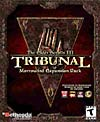
\includegraphics{media/image6.png}

{[}no fix?{]} SetDelete flag\_enum

SetDelete 1

The SetDelete function can be used in combination with Disable to remove
an object more completely. SetDelete 1 marks a reference for deletion
and SetDelete 0 clears that flag. This can be useful in optimization.
Certain objects have scripts on them which simulate picking them up by
disabling the activated reference and adding a new object to your
inventory. This leaves an ever-present, but disabled, reference at that
location (which eats up memory and processor time since the script on
the disabled reference is still run every frame). If the reference is
marked for deletion then it is essentially gone. If the reference came
from the master file, it is still there but knows it shouldn't be so has
no art and no scripting. If was created in game, it will actually be
deleted.

\textbf{Notes and cautions:}

SetDelete will crash Morrowind if there is any other function operating
on the object in the same frame. It will also crash if the object emits
sounds (or plays animations with linked sounds) and is disabled and
deleted in the same frame (forum info / JOG).

This Script \textbf{will crash}:

\lstinputlisting{scripts/_spell_effect01.txt}

A solution is to use first disabling the object and then using
GetDisabled and Return to safely delete the object:

\lstinputlisting{scripts/_spell_effect02.txt}

Another solution was proposed by Soralis, using a local variable
"deletobj" as a flag:

% Put in listlistings?

if ( deleteobj = 1 ) ;Local variable, set when you want to delete

if ( deletetimer == 0 )

Disable

endif

if ( deletetimer < 10 )

set deletetimer to ( deletetimer + 1 )

endif

if ( deletetimer == 10 )

\textbf{SetDelete}, 1

endif

Return

endif

Always call SetDelete from a local script assigned to the object you
want to remove. Never use Object-> SetDelete 1 as this
usually causes crashes when Morrowind is running. However, starting a
targeted script on the object and then using SetDelete in that script
works fine.

Don't delete items in inventory: this results in incorrect encumbrance.
If necessary, Drop can be used to remove the item from inventory before
deletion.

It has been reported that magic effects can cause problems with
SetDelete (forum info / Dan\_Wheeler). I (melian) am not sure exactly
what this refers to, but I do know that if an NPC is deleted too quickly
after another NPC casts a spell on it (scripted cast), the game will
crash. If this causes you problems, use a timer to wait before deleting
the object (you may need to wait a few seconds).

\hypertarget{dont-save-changes-to-an-object}{%
\subsection{\texorpdfstring{\hfill\break
Don't save changes to an
object}{ Don't save changes to an object}}\label{dont-save-changes-to-an-object}}

DontSaveObject

Call this function if changes to the object are not to be saved to the
savegame.\\
Use DontSaveObject on objects that:

1. Can be enabled/disabled during the game, such as the stages of
building a stronghold.

2. Objects that might be moved, such as rideable objects.

By using DontSaveObject you will avoid that annoying "save game data has
changed" error message that will occur when load a saved game and the
object's state has changed, ie: it has moved, or has been
disabled/enabled. This is due to the fact that object data is stored in
the save game data, such as if the object is enabled or disabled, or if
it has been moved (like a rideable object) (Forum info / IndigoRage).

In the original game, it's used in the SignRotate script and the
following one:

Sample Script:

\lstinputlisting{scripts/diseaseAscended.txt}

\hypertarget{scripting-npcs-ai-and-movement}{%
\section{\texorpdfstring{\hfill\break
Scripting NPCs: AI and
Movement}{ Scripting NPCs: AI and Movement}}\label{scripting-npcs-ai-and-movement}}

\hypertarget{make-an-npc-walk-to-a-new-location}{%
\subsection{Make an NPC walk to a new
location}\label{make-an-npc-walk-to-a-new-location}}

AiTravel, float\_enum\_x, float\_enum\_y, float\_enum\_z, {[}reset{]}

Actor-> AITravel, 1359, 2700, 1045

To make an NPC walk between different defined places in the game world
you use the AITravel function.

The variables x, y, z are world coordinates. You can determine these by
moving your camera to the desired endpoint of the movement or by
selecting a path grid point or an object nearby coordinates are
displayed below the object window. The usage of the optional reset flag
is unknown.

When using this function in scripts it is important to provide
conditions where the AI package is called only once. Consider the
following NPC bound script

\lstinputlisting{scripts/Travel01.txt}

The previous script will not work, as the script ``fires'' continuously,
and the effect is that the NPC freezes and never performs the desired
movement.

\lstinputlisting{scripts/Travel02.txt}

This should work; the NPC will wander to the designated coordinates as
soon as his script becomes active, meaning as soon as his cell is
loaded.

\hypertarget{checking-whether-an-npc-has-performed-his-movement}{%
\subsubsection{Checking whether an NPC has performed his
movement}\label{checking-whether-an-npc-has-performed-his-movement}}

GetAIPackageDone (returns Boolean/short)

if ( GetAIPackageDone == 1 )

{[}do something{]}

endif

To check whether an NPC has arrived at his location you can use the
\emph{GetAIPackageDone} function. This function returns 1 for one frame
when the current AI package has finished.

Use this to perform a check whether a movement has been finished. The
following script is an example of how to link several \emph{AITravel}
commands within one script, using a state variable and an
\emph{if-elseif} structure:

\lstinputlisting{scripts/TravelLoop.txt}

Good examples of scripting using \emph{AITravel} are also found in the
``lookoutscript'' (Fargoth hiding his treasure) and the CharGenWalkNPC
script (The guard that walks you through the ship at the beginning of
the game). Or look at my "Traveling Merchants" plugin for true AITravel
madness !

If you plan on using this function extensively you should be aware of
the following problems: When you leave a cell with an Actor that is just
performing its AITravel command, or if you rest, the script will never
detect the \emph{GetAIPackageDone} signal, meaning your NPC gets stuck
on its path once you return or finish sleeping. The following simple
code can be used to get the script going again (this is for the above
script)

% Excerpt from external script

; *************** Stalled Script rescue - recovers script after leaving
a cell or resting

If ( Player-> GetDistance, HB\_adros\_darani < 5000
)

if ( GetCurrentAIPackage == -1 ) ; check for idleness

set timeout to ( timeout + GetSecondsPassed )

if ( timeout >= 3 ) ; wait some time.

; Short instances of idleness always occur

set state to ( state - 10 ) ; stall will occur at ; AIPAckageDone - jump
to "wander" again.

set timeout to 0

endif

else

set timeout to 0

endif

endif

\hypertarget{make-an-actor-turn-or-face-a-certain-direction}{%
\subsection{Make an Actor turn or face a certain
direction}\label{make-an-actor-turn-or-face-a-certain-direction}}

Face x\_enum, y\_enum

"ActorID"-> Face, -1334, 334

To my knowledge this function does not accept variables (at least under
version 1.6.1820), but there have been reports that it did - possibly
this is version dependent. This function Makes an NPC face towards a
specified x/y coordinate. Apparently interrupts current animations.
Using this on wandering NPCs makes them stop, face wherever, then
continue on wherever they were wandering to, as soon as the facing
movement is over. (Forum info / JOG, Dan\_Wheeler).

\hypertarget{define-random-actor-movement}{%
\subsection{Define random Actor
movement}\label{define-random-actor-movement}}

AiWander, range\_enum, duration\_enum, time\_enum, {[}idle1{]},
{[}idle2{]}, {[}idle3{]}, \ldots{[}idle9{]}, {[}reset{]}

"Actor\_ID"-> AIWander, 512, 5, 0, 0, 20, 0, 0, 10, 30, 0, 0,
0

This is the random movement algorithm that most of the NPCs in the game
are using. The NPC travels along the path grid, changes direction
randomly, and performs idle movements in between.

\begin{itemize}
\item
  Range: determines the distance the Actor or creature will roam from
  his origin.
\item
  Duration: probably the time (in hours) the mob will perform the
  package (before it is reset, which seems to happen if you leave or
  sleep, not sure?)
\item
  time: presumably determines the start time for the package if it has a
  duration
\item
  {[}idle1{]}, \ldots{[}idle9{]}: chances of idle movements.\\
  \strut \\
  The Idles are (as tested in game):
\item
  Human male:\\
  Idle1: Stand still\\
  Idle2: Shifting weight from one leg to the other\\
  Idle3: Looking behind\\
  Idle4: Scratching head, shake head\\
  Idle5: Shifting clothing or armor on shoulder\\
  Idle6: Yawning and stretching\\
  Idle7: Looking at fingers and looking around furtively\\
  Idle8: Putting hand to chest, as if having heartburn\\
  Idle9: Reaching for weapon, then touching head
\item
  Human female - as above but:\\
  Idle5: Hand on hip
\item
  Khajiit female - as Human male but\\
  Idle9: Scratching head, shaking head
\end{itemize}

To let an Actor stand in one spot you can use: AIWander, 0, 0, 0

\textbf{Note:} The number of idles and some of the descriptions were
listed wrongly in previous versions (corrected with
8\textsuperscript{th} edition - credits go to Whoopa).

Here is an \textbf{example script} that displays all idles in series
(this my be useful to check out which ones you want your NPC to use):

\lstinputlisting{scripts/Animtest.txt}

\hypertarget{making-actors-activate-objects}{%
\subsection{\texorpdfstring{\hfill\break
Making Actors activate
objects}{ Making Actors activate objects}}\label{making-actors-activate-objects}}

AiActivate "Object ID"

AiActivate ObjectID {[}reset{]}

Actor-> AIActivate "Object"

In the words of Bethesda: "This package tells the Actor to activate the
specified ObjectID. A powerful and admittedly underutilized and
undertested package."

In standard Morrowind this function appeared to be mostly broken, except
for making an NPC quaff a potion. \textbf{With Tribunal} it seems to
have been fixed, at least to some extent. I could successfully use it to
get an NPC to pick up a weapon, open a normal door and go through a load
door. LoadDoors only work if the door marker it teleports to is in the
same interior cell, or within the loaded (PC's current and surrounding)
cells in exterior cells -- otherwise the game crashes. I also tested it
successfully with an activator (switch to open Ghostgate).

The usual precautions with AI functions apply (make sure the Actor is
not too far away, have a good AI grid in place, make sure nothing can
get in the way, etc.). Although not thoroughly tested, I didn't seem to
get an \emph{AIPackageDone} signal, but other conditions can be
constructed (see examples below) to set the NPC to a different AIPackage
again.

\begin{longtable}[]{@{}
  >{\raggedright\arraybackslash}p{(\columnwidth - 2\tabcolsep) * \real{0.25}}
  >{\raggedright\arraybackslash}p{(\columnwidth - 2\tabcolsep) * \real{0.75}}@{}}
\toprule
\begin{minipage}[b]{\linewidth}\raggedright
Object Type
\end{minipage} & \begin{minipage}[b]{\linewidth}\raggedright
Activation
\end{minipage} \\
\midrule
\endhead
NPC & Activating NPC will approach and circle the target NPC \\
Container & Opens \\
Door & Opens \\
Load door & Opens/teleports (same cell only) \\
Weapon, armor, misc., etc & Picks up \\
Book/Scroll & Reads < meaning what to an NPC?> \\
Activators & Execute as defined by script. If the activator doesn't have
an OnActivate block (or doesn't have a script), the Actor will try to
activate it anyway, in much the same way as 'activating' NPCs (approach
and circle). \\
\bottomrule
\end{longtable}

\textbf{Note:}

If you place the object to be activate too high, the NPC will still
approach and circle underneath it.

\textbf{Sample Script:} these are just a few testing scripts I made.
They show how you can set conditions to determine when the NPC has
finished his action.

\lstinputlisting{scripts/TT_opendoor.txt}

\lstinputlisting{scripts/TT_pickmace.txt}

\lstinputlisting{scripts/TT_openloaddoor.txt}

\hypertarget{following-and-escorting}{%
\subsection{Following and Escorting}\label{following-and-escorting}}

AiFollow, "Actor ID", duration\_f\_enum, x\_f\_enum, y\_f\_enum,
z\_f\_enum, {[}reset{]}

AiFollowCell, "Actor ID", "Cell ID", duration\_f\_enum, x\_f\_enum,
y\_f\_enum, z\_f\_enum, {[}reset{]}

Actor-> AIFollow, "Mob2ID", 0, 0, 0, 0

The "Follow" AI-package makes an Actor closely follow another. You can
use this to make an NPC or creature follow the player, but you can also
use it to make NPCs and creatures form a caravan. The following excerpt
from one of my own scripts shows the unconditional use of the function:

elseif ( state == 20 )

HB\_guar\_pack\_adros\_->\textbf{AIFollow},
HB\_adros\_darani, 0, 0, 0, 0

AITravel -8144, -19409, 728 ;new coords point 1

set state to 30

Since there is no duration or destination location given, the guar will
follow the NPC until another command is given. As with other
AI-commands, make sure you set conditions so that each AIFollow command
is issued only once, not every frame.

The duration, CellID and x, y, z destination coordinates set conditions
that once fulfilled will terminate the AIPackage (which you can test
with the GetAIPackageDone function as describe for AITravel above). The
AiFollowCell function allows you to set an interior cell as the
destination.

The meaning of the optional reset option is currently unknown.

AIEscort, "Actor ID", duration, x, y, z, {[}reset{]}

AIEscortCell, "Actor ID", "Cell ID", duration, x, y, z, {[}reset{]}

This function makes an Actor lead another actor or the player to a
certain point. The Actor will wait for the follower if the distance
becomes too great, and will resume its path when the follower approaches
again (Thanks to Kir for this info). You see an \textbf{example} of this
in character generation: the guard who escorts you up from the ship's
hold to the ramp on the second level. (Thanks to MisterSmileyFaceDude).
The meaning or use of {[}reset{]} is unknown.

\hypertarget{checking-which-ai-package-is-currently-executed}{%
\subsection{Checking which AI package is currently
executed}\label{checking-which-ai-package-is-currently-executed}}

For complex Actor scripting it might be valuable to know which AI mode
is currently active and make script actions dependant on it.

GetCurrentAIPackage (returns short)

If ( GetCurrentAIPackage == 2 )

{[}do something{]}

endif

The returned values are:

\begin{longtable}[]{@{}
  >{\raggedright\arraybackslash}p{(\columnwidth - 2\tabcolsep) * \real{0.72}}
  >{\raggedright\arraybackslash}p{(\columnwidth - 2\tabcolsep) * \real{0.28}}@{}}
\toprule
\endhead
None & -1 \\
Wander & 0 \\
Travel & 1 \\
Escort & 2 \\
Follow & 3 \\
Activate & 4 \\
Pursue & 5 \\
\bottomrule
\end{longtable}

\hypertarget{section-6}{%
\paragraph{}\label{section-6}}

Casey Tucker wrote a few interesting notes about Morrowind's AI system:

\emph{These are a few notes on Morrowind's AI system, as much for myself
as for anyone wishing to look them over. The most I noticed the AI is
incredibly stubborn. There are quite a few unpredictable script
functions that deal with AI. I find that the AIFollow is actually the
most stable of them.}

\emph{\hfill\break
When working on "The Triumvirate" quest/war mod, if the player went to
Dragonhold Castle to join the Legion, I had to have the player's
Imperial Centurion, Sensius Tanarii, show the player where his barracks
room is.}

\emph{\hfill\break
Initially I had Sensius follow the player until you wandered around long
enough to find your barracks room. Sensius would confirm the location
and disappear, once Proximus Taiatius, (your legionary roommate) noticed
you.}

\emph{(GetTarget Player == 1 Usually works - For the desired effect,
GetDistance is more accurate.)}

\emph{\hfill\break
So, that was sort of the opposite of I wanted. I wanted Sensius to take
the player to their room. When I first actually thought of this, I tried
thinking of several ways to get an NPC to "AiEscort" through several
cells to the given coordinates. Let me tell you of my findings on
AIEscort. It's either broken, works only in exterior cells, or I was
doing something wrong. Regardless, I noticed that the NPC did not budge
at all from their location, though they WERE set to guard the player.
Upon further research, I saw that during the CharGen process, when the
prison ship guard appears to be escorting you to the door, Bethesda
actually used AIWander, making checks to see if the player was following
or not.}

\emph{From this I drew the conclusion that AITravel would be so much
more convenient and stable. I only use AIEscort to get a stationary
actor to guard the player if they came under attack. Useful for battle
scenes when you want it to appear that two forces are fighting each
other, without having an entire side follow the player. About mass
battles... I will lead into that later.}

\emph{\hfill\break
First, I must explain how to get an NPC to escort a player, from point
A: an interior cell, through several interior and exterior cells, to
point B: also an interior cell. First things first.. we don't want the
NPC to get stuck. You'll need some pathgrids. A few notes about
pathgrids: the NPC doesn't seem to care about the gridpoints' Z
coordinate {[}This doesn't appear to be correct. See notes below{]}.
That's a very good thing. Pathgrids are like magnetic roads. The NPC is
seemingly "magnetically attracted" to that pathgrid, and their
AIWandering, AITraveling, and AIFollowing will follow along those grids.
To see how these grids work, go in-game, to Ebonheart or another
semi-crowded city, and type in the console: 'TPG'. That will show the
pathgrids - you'll see the NPC's walking between the two yellow "rails"
that are drawn out, as if they were trains. An NPC will reluctantly pull
away from a pathgrid if led so by the player, need to walk around
something blocking their way, chasing someone/thing, and such
scenarios.}

Now that I got pathgridding done, I noticed another thing. AITravel is
not "unstable" per se, but not very reliable. Two factors come into play
here, that dictate if the NPC will blatantly ignore it's orders or do as
told. The first, I noticed, was the AI distance setting, changeable by
FPS optimizer or in-game menu. Makes sense. However, the next one is
rather annoying. The NPC cannot get distracted or their travel will
stop. This means you'll have to set their "Hello" distance to 0 during
their little stroll, otherwise they will stop and greet the player
instead.

\emph{\hfill\break
Now we come to the point where the NPC reaches a load door through
cells. The game will CTD if the NPC activates it. Here is a snippet of
an "escort" script I wrote, that gets the NPC through a load door.}

\lstinputlisting{scripts/Sensius_Escort_Script.txt}

That should explain how it would work. Coordinates are often more
reliable than a "GetAIPackageDone" function, mainly because that
function is easily broken by several factors.

Some notes on the notes (!)

\begin{itemize}
\item
  It's been reported by others (and I've found myself) that the z-pos of
  pathgrid nodes \textbf{does} matter (at least in interiors): if a node
  isn't well above the floor the actor can get "stuck" at that point and
  refuse to move past it.
\item
  AIEscort has been used successfully by a number of modders (and in
  Bethesda's scripts, e.g. CharGenWalkNPC). That's not to say it's
  without problems, but it is certainly useable. However, since AIEscort
  may not be viable in some circumstances, the above notes may help you
  develop an alternative approach should one be necessary.
\end{itemize}

\hypertarget{forcing-sneak-movement}{%
\subsection{Forcing sneak movement}\label{forcing-sneak-movement}}

ForceSneak

ClearForceSneak

"Actor\_ID"-> ForceSneak

GetForceSneak ( returns Boolean/short)

If ( "actor\_ID"-> GetForceSneak == 1 )

The \emph{ForceSneak} command puts the Actor in sneak mode, all movement
will be performed in sneaking. \emph{ClearForceSneak} terminates
\emph{ForceSneak} mode. Unfortunately there does not seem to be a
corresponding command to force running (added with Tribunal).
\emph{GetForceSneak} returns one if \emph{ForceSneak} mode is active on
the calling Actor. Check the LookoutScript script for an example. Here's
a snippet:

elseif ( walkstate == 2 )

Fargoth-> ForceSneak ; enter sneak mode

Fargoth-> AiTravel -11468.595,-71511.531,173.728 ;goes to
tree

set walkstate to 3

elseif ( walkstate == 3 )

if ( Fargoth-> GetAiPackageDone == 1 )

;Fargoth-> Equip "torch\_infinite\_time\_unique"

set walkstate to 4

;MessageBox "SHOULD BE AT TREE"

endif

elseif ( walkstate == 4 )

set timer to timer + GetSecondsPassed

Fargoth->\textbf{ClearForceSneak} ; terminate sneak mode

Fargoth-> AiWander 0 0 0 0 0 0 0 0 0

if ( timer > 3 )

Fargoth->\textbf{ForceSneak} ; reenter sneak mode

Fargoth-> AiTravel -11410.590,-72057.188,133.644 ;goes to
wall

set walkstate to 5

endif

\hypertarget{forcing-running-and-jumping-tribunal-npc-movement-functions}{%
\subsection{\texorpdfstring{\hfill\break
Forcing running and jumping: Tribunal NPC Movement
Functions}{ Forcing running and jumping: Tribunal NPC Movement Functions}}\label{forcing-running-and-jumping-tribunal-npc-movement-functions}}

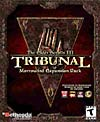
\includegraphics{media/image6.png}

ForceRun

ClearForceRun

GetForceRun (short)

ForceJump

ClearForceJump

GetForceJump (short)

ForceMoveJump

ClearForceMoveJump

GetForceMoveJump (short)

These functions all control the specified NPC's movement. The ForceRun
function makes the NPC always run when they move, the ForceJump function
makes the NPC constantly jump, and the ForceMoveJump makes the NPC
always jump when they are moving. The Get versions of the functions
return one if the specified NPC currently is forced into the given
action and zero otherwise. The Clear functions are used to turn forced
movement modes off. An NPC can only be forced to do one movement at a
time. The priority for forced movement is Sneak > Running
> Jump > MoveJump.

Sample Script:

This script lets an object control the movement type of Athlete, an NPC
set to Travel endlessly in a four-point square.

\lstinputlisting{scripts/AthleteControl.txt}

\hypertarget{detecting-players-action-running-jumping-sneaking}{%
\subsection{Detecting players action: running, jumping,
sneaking?}\label{detecting-players-action-running-jumping-sneaking}}

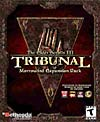
\includegraphics{media/image6.png}

{[}no fix{]} GetPCSneaking (short)

{[}no fix{]} GetPCRunning (short)

{[}no fix{]} GetPCJumping (short)

if ( GetPCRunning )

These functions returns 1 if the PC is performing the appropriate action
and 0 if he is not. Since Morrowind doesn't have functions to directly
test for keyboard input, these functions provide an alternative to check
if the player has a certain button pressed. They have accordingly been
used extensively for control purposes, e.g. for movable ships, ridable
creatures, or in my climbing mod.

Sample script:

When this script is placed on an NPC, and the player has an item
equipped called ``scissors'', MessageBox warnings will be given based on
the player's current actions.

\lstinputlisting{scripts/momscript.txt}

\hypertarget{detect-combat-readiness}{%
\subsection{Detect combat readiness}\label{detect-combat-readiness}}

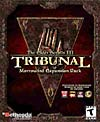
\includegraphics{media/image6.png}

GetWeaponDrawn (short)

GetSpellReadied (short)

if ( player-> GetWeaponDrawn )

These functions can be used to determine whether or not an Actor has
their weapon out or whether or not they have a spell readied for
casting.

Sample Script: This global script gives notification messages based on
the player's weapon and spell states.

\lstinputlisting{scripts/player_notifications.txt}

\textbf{Note:} GetWeaponDrawn will return 0 at some unusual times; when
a lock pick or probe is removed through scripting or when it is broken,
GetWeaponDrawn will return 0 for a few frames before you switch to
Hand-to-Hand. When fighting Hand to Hand, when you equip or remove a
piece of armor or clothing, GetWeaponDrawn will return 0 briefly.\\
Thanks to Björn and DinkumThinkum respectively for pointing this out.

\hypertarget{section-7}{%
\subsection{}\label{section-7}}

\hypertarget{making-someone-fall}{%
\subsection{Making someone fall}\label{making-someone-fall}}

Fall

Actor-> Fall

Seems to give an NPC the extra nudge they may need even after you yank
the floor out from under them. It also brings down flying creatures.
Used by the Icarian Flight guy. When I tried to use this on the player
in my climbing mod, it seemed to sometimes "warp" the player directly to
the ground below.

\hypertarget{equipment-sharing-and-other-companion-functions}{%
\subsection{Equipment sharing and other companion
functions}\label{equipment-sharing-and-other-companion-functions}}

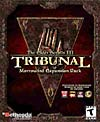
\includegraphics{media/image6.png}

{[}no fix{]} companion (is local short)

short companion

Set companion to 1

Tribunal introduced the option to "share" equipment with NPC's or
creatures. To enable this option, you must define a local short variable
named "companion" and set it to 1 or higher. Setting it to 0 or a
negative value will disable sharing. This method is used both for
mercenaries and for pack animals.

{[}no fix{]} minimumprofit (is local float)

Float minimumprofit

If ( minimumprofit < 0 )

Seems to be another variable set by the game, it is probably the
difference between current value of all goods and gold minus starting
value. If this gets negative, the mercenary can be scripted to quit.

\textbf{Sample Script:} here is the relevant part from Calvus' script
(the mercenary in Mournhold). This section handles changes in state when
Calvus leaves a contract, either because the contract expires, or
because the player has taken Calvus' stuff. The sharing is initiated
from dialogue (setting companion to 1), not in the script itself

% Put in listlistings?

if ( GetJournalIndex Merc\_Calvus\_Quit < 1 ) ;if Calvus has
already quit, don't do this

if ( Contract\_Calvus == 1 ) ;if Calvus doesn't have a contract, don't
do this

if ( \textbf{minimumProfit} < 0 ) ;Calvus is quitting because
player took his stuff

AiWander 128 6 0 40 30 20 0 0 0 0 0 0

\textbf{Set Companion to 0;} stop sharing

StopScript Contract\_Calvus

Set Contract\_Calvus to 0

ForceGreeting

return

else

if ( Contract\_Calvus == 0 ) ;handles Calvus after a contract expires

AiWander 128 6 0 40 30 20 0 0 0 0 0 0

\textbf{Set Companion to 0;} stop sharing

if ( GetJournalIndex Merc\_Calvus < 10 )

Journal Merc\_Calvus 10 ;first contract expired

else

Journal Merc\_Calvus 20 ; most recent contract expired

endif

endif

endif

endif

endif

{[}no fix{]} StayOutside (is local short)

short StayOutside

set StayOutside to 1

A useful variable for companions. When used in a script, it causes
whoever it's assigned to to automatically remain (and wait) outside of
any interior the player may enter (automatically rejoins upon return).
(Forum info / Grumpy)

\hypertarget{race-faction-and-rank}{%
\section{\texorpdfstring{\hfill\break
Race, Faction and
Rank}{ Race, Faction and Rank}}\label{race-faction-and-rank}}

\hypertarget{determining-race}{%
\subsection{Determining Race}\label{determining-race}}

GetRace, ``RaceID'' (returns Boolean/short)

Player-> GetRace "Dark Elf"

Returns 1 if the object is of the race indicated by RaceID.

Sample Script: This is a global script Bethesda uses to set a variable
that can be used to determine the PCs race in dialogue:

\lstinputlisting{scripts/RaceCheck.txt}

\hypertarget{determining-the-pcs-faction-status}{%
\subsection{Determining the PC's Faction
status:}\label{determining-the-pcs-faction-status}}

{[}no fix{]} GetPCRank, FactionID\_enum (returns short)

if ( GetPCRank "Telvanni" == 9 )

Returns PC's rank in faction. This will default to the Actor's faction
if FactionID is not defined. Returns 0-9 and -1 if not a member.

Sample Script: An Actor/object with the following script is only enabled
if the PC is not a member of House Redoran:

\lstinputlisting{scripts/bandenIndarysScript.txt}

{[}no fix?{]} GetPCFacRep, {[}FactionID{]} (returns short?)

This \textbf{doesn't work} in script (causes errors and/or crashes when
used).

SameFaction (returns Boolean/short)

Returns 1 if PC is in the faction of the calling object (NPC).

PCExpelled {[}"factionID"{]} (returns Boolean/short)

Returns 1 if PC has been expelled once from calling object's (NPC)
Faction, or a faction can be defined to get a specific one. For an
example script look below, PCClearExpelled function.

\hypertarget{modifying-faction-standing-and-reaction}{%
\subsection{Modifying faction standing and
reaction}\label{modifying-faction-standing-and-reaction}}

{[}no fix{]} PCJoinFaction {[}"FactionID"{]}

Makes the PC a member of the specified faction. FactionID is optional if
it is not added it will use the faction of the NPC who called the
function

LowerRank, {[}"FactionID"{]}

RaiseRank, {[}"FactionID"{]}

Raises or lowers the object's rank in its current faction. This function
doesn't work in global scripts, but works in targeted and local scripts.
It also works in dialogue. You can use the fix to raise a different
NPC's rank (NPC\_ID-> RaiseRank) in dialogue results
\textbf{only} - in scripts this function will only work on the actor the
script is attached to.

The faction ID argument is totally ignored by the game engine, so is not
required, and even if you have the faction ID as something totally
irrelevant (for example ``eel pie''), the script still compiles and runs
fine.

You cannot use RaiseRank to have an NPC join a faction (unlike the PC
version) - if the NPC doesn't already belong to a faction RaiseRank has
no effect.

{[}no fix{]} PCLowerRank, {[}"FactionID"{]}

{[}no fix{]} PCRaiseRank, {[}"FactionID"{]}

Raises or lowers the PC 1 rank in the NPCs faction. If PC is not part of
the faction, it will set the rank to 1.

\textbf{Example Script:}

\lstinputlisting{scripts/treboniusScript.txt}

{[}no fix{]} PCExpell {[}"FactionID"{]}

Expels PC from NPCs faction.

{[}no fix{]} PCClearExpelled {[}"FactionID"{]}

Clears "currently expelled" flag on the player.

Example script:

A script by Bethesda, which clears the Players expelled status after
some time:

\lstinputlisting{scripts/expelledMG.txt}

{[}no fix{]} ModPCFacRep, var\_enum, {[}"FactionID"{]}

{[}no fix{]} SetPCFacRep, var\_enum, {[}"FactionID"{]}

ModPCFacRep, 5, "Imperial Legion"

ModPCFacRep, 5, "Temple"

Modifies or defines the reaction modifier for members of the specified
faction (towards the PC).

ModFactionReaction, "factionID1", "factionID2", var\_enum

SetFactionReaction, "factionID1", "factionID2", var\_enum

Modifies or defines the reaction of one faction towards members of
another faction.

\textbf{Example}: This is part of the MoonAndStar script. This part
first makes the PC part of the faction "Nerevarine" and then sets two
factions to react particularly to this change:

;faction reaction and journal stuff

Journal "A2\_6\_Incarnate" 50

player-> modReputation 5

\textbf{PCJoinFaction}, Nerevarine

if ( GetPCRank, Redoran >= 0 )

\textbf{modFactionReaction}, "Redoran", "Nerevarine", 4

endif

if ( GetPCRank, Temple >= 0 )

\textbf{modFactionReaction}, "Temple", "Nerevarine", 4

endif

\hypertarget{determining-and-changing-reputation-and-disposition}{%
\subsubsection{Determining and changing reputation and
disposition}\label{determining-and-changing-reputation-and-disposition}}

\emph{Get/Mod/Set}Reputation

\emph{Get/Mod/Set}Disposition

SetDisposition refers to base disposition (as set in the TES CS,
unaltered by any modifiers). To set the disposition value used in game,
use a combination of GetDisposition (returns current value) and
ModDisposition; for example, to completely control an NPC's disposition
from a global "myRealDisp" (can be a short, it doesn't need to be a
float unless you want to change disposition by float values), the NPC's
local script could include something like this:

if ( myRealDisp > 100 )

set myRealDisp to 100

elseif ( myRealDisp < 0 )

set myRealDisp to 0

endif

set localFloatVar to ( GetDisposition )

set localFloatVar to ( myRealDisp - localFloatVar )

ModDisposition localFloatVar

\emph{\hfill\break
}

\hypertarget{werewolf-specific-functions}{%
\subsection{Werewolf-specific
functions}\label{werewolf-specific-functions}}

\hypertarget{set-the-werewolf-attributes}{%
\subsubsection{Set the werewolf
attributes}\label{set-the-werewolf-attributes}}

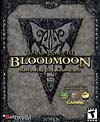
\includegraphics{media/image7.png}

SetWerewolfAcrobatics

Actor-> SetWerewolfAcrobatics

This function set the attributes of the object to those of a werewolf.
This sets the targets skills and attributes to match the fWerewolfxxxx
gameplay settings. In most cases, this means a high strength, agility,
acrobatics etc, and 0 in most other things.

Player-> AddSpell "werewolf vision"

Player-> AddSpell "werewolf regeneration"

Player-> SetWereWolfAcrobatics

\hypertarget{change-the-color-of-secunda}{%
\subsubsection{Change the color of
Secunda}\label{change-the-color-of-secunda}}

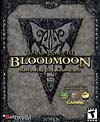
\includegraphics{media/image7.png}

{[}no fix{]} TurnMoonWhite

{[}no fix{]} TurnMoonRed

These two functions are very simple -- they change the color of Secunda
(The small, white moon) from white to red and back again. This doesn't
have any real effect to gameplay, but it does make the sky look
different. It is used during the Bloodmoon main quest -- hence the
expansion title.

if ( doOnce == 0 )

TurnMoonRed

set doOnce to 1

endif

\hypertarget{determine-how-many-kills-a-werewolf-has}{%
\subsubsection{Determine how many kills a werewolf
has}\label{determine-how-many-kills-a-werewolf-has}}

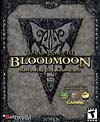
\includegraphics{media/image7.png}

{[}no fix{]} GetWerewolfKills (returns short ?)

This keeps count of how many NPC's killed by the player when in werewolf
form. Each time an NPC is killed while the PC is a werewolf, one is
added to this count. It is reset automatically when the PC changes back
into human form.

if ( GetWerewolfKills > 0 )

; Do code to stop the PC from being affected by the hunger.

endif

\hypertarget{check-to-see-if-the-creature-is-in-werewolf-form}{%
\subsubsection{Check to see if the creature is in werewolf
form}\label{check-to-see-if-the-creature-is-in-werewolf-form}}

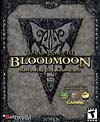
\includegraphics{media/image7.png}

IsWerewolf

If ( Actor-> IsWerewolf )

This function allows to determines if the target is a werewolf or not.
It can be used on the PC or other creatures.

if ( Player-> IsWerewolf != 1 ) ;DON'T RUN IF PLAYER ISN'T
WEREWOLF

return

endif

\hypertarget{change-to-a-werewolf}{%
\subsubsection{Change to a werewolf}\label{change-to-a-werewolf}}

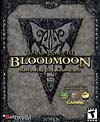
\includegraphics{media/image7.png}

BecomeWerewolf

UndoWerewolf

Actor-> BecomeWerewolf

Actor-> UndoWerewolf

These functions change the target object to a Werewolf or change them
back to their original form. IMPORTANT: Using Becomewerewolf and
Undowerewolf CAN break your game. Some quests and variables depend
solely on use of these, so if you use one to toy around.... you may be
asking for it. (This message brought to you by your friendly dev
WormGod).

Note:

When the player is a werewolf, the only thing you can detect them
activating (Using OnActivate) is doors.

If you want to detect the player activating an object, or even another
werewolf, one method is to use an invisible door and place it over the
object you want to detect the activation of.

if ( OnPCEquip == 1 )

Player-> BecomeWereWolf

Set OnPCEquip to 0

Endif

Set timer to ( timer + GetSecondsPassed )

If ( timer > 10 )

Player-> UndoWereWolf

Endif

\hypertarget{section-8}{%
\subsubsection{}\label{section-8}}

\hypertarget{section-9}{%
\subsubsection{}\label{section-9}}

\hypertarget{section-10}{%
\subsubsection{}\label{section-10}}

\hypertarget{special-werewolf-global-variables}{%
\subsubsection{Special werewolf global
variables}\label{special-werewolf-global-variables}}

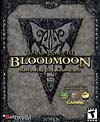
\includegraphics{media/image7.png}

{[}no fix{]} PCknownWerewolf (is short global)

A global variable that indicates whether the PC is a known werewolf

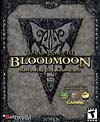
\includegraphics{media/image7.png}

{[}no fix{]} PCWerewolf (is short global)

Set to 1 when player is werewolf. Used in controlling numerous werewolf
scripts.

It works in the same way as PCVampire:

-1 = Player has been cured of lycanthropy and cannot become a werewolf
again

0 = Player is not a werewolf

1 = Player is a werewolf

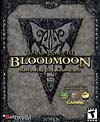
\includegraphics{media/image7.png}

{[}no fix{]} WerewolfClawMult (is float global)

A multiplier for claw damage. Exact formula unclear, see werewolf
scripts for reference.

\hypertarget{text-and-dialogue}{%
\section{\texorpdfstring{\hfill\break
Text and Dialogue}{ Text and Dialogue}}\label{text-and-dialogue}}

\hypertarget{brief-dialogue-how-to}{%
\subsection{Brief dialogue how-to}\label{brief-dialogue-how-to}}

Dialogue is an art in itself that can not be fully covered here.
However, when creating quests you will often mesh dialogue and scripting
to control your quest and achieve certain effects. Therefore, I will
give a brief introduction.

\hypertarget{the-concept-of-mw-dialogue}{%
\subsubsection{The concept of MW
dialogue}\label{the-concept-of-mw-dialogue}}

In Morrowind, dialogue is organized in a database. This database is
structured in the following way:

Top level:

The different "divisions" of dialogue are:

\emph{Topic:} The actual topic words and responses for the dialogue
window in the game.

\emph{Greetings:} The text strings you are greeted with when you
initiate dialogue with an Actor.

\emph{Persuasion:} The answers you get for successful or failed
persuasion attempts.

\emph{Journal:} The entries for your journal.

\emph{Voice:} The .mp3 sound files (and subtitles) that players "say"
when you come near, are hit, are fleeing, etc.

Find these divisions on the tabs on the top left of the dialogue window
(use the arrows to get to the hidden tabs).

Sub-level 1:

Each of these top level divisions has sublevels I call topics -- for the
\emph{Topics} division, these are the actual "keywords" (topics) that
Actors will have something to say about. These are the words that will
be highlighted ("hyperlinked") in in-game text and listed in the right
hand panel of the dialogue window. For \emph{Journal} these are the
different journals (usually one per quest). For \emph{Voices} the
different categories of sound responses that are "triggered" by the
appropriate in-game conditions etc. For \emph{Greetings} these are just
general categories of greetings (diseased, quest offers, standard and so
on). This is the way Bethesda has used them (forum info / Emma):

\begin{itemize}
\item
  Greetings 0: Npc is alarmed
\item
  Greetings 1: Quests (actually quests where it doesn't matter if the
  Player is a vampire, is nude, is a criminal, is diseased).
\item
  Greetings 2: Player is a vampire/player is nude
\item
  Greetings 3: Traitors to Morag Tong
\item
  Greetings 4: Crime and disease
\item
  Greetings 5: Quests
\item
  Greetings 6: Factions
\item
  Greetings 7: Classes, Endgame, Slaves
\item
  Greetings 8: Clothes (general greetings concerning how player is
  dressed)
\item
  Greetings 9: Locations.
\end{itemize}

For \emph{Persuasion} these are things like service refusals or bribe
success/fail messages.

Sub-level 2:

For each topic there can be one or several sub-entries ("Info/Response")
-- these are the actual responses. For \emph{Topic} and \emph{Greetings}
these are the actual answers of Actors to the topic phrase. For
\emph{Journal} these are the different entries describing the progress
of a quest.

These entries represent a linked list, meaning that each entry contains
(invisible) info on which is the next response in line and which is the
previous. (This leads to a common error message when dialogue gets
deleted or scrambled, e.g. by cleaning a mod with TESAME, or by loading
several mods that change the same topic. The game doesn't know for sure
any more which entry comes after which. This sometimes doesn't matter,
but it can also mean that certain responses are cut off, because the
order isn't right any more -- this depends on the conditions). To check
and/or change the next/previous ID strings, you can export the dialogue
and re-import it if necessary (solution suggested by Kateri).

Dialogue entries come with conditions that you can set in the dialogue
editor window. In the topic window you will find a list of general
conditions on the left -- here you can define which Actor (Actor ID) or
group of Actors (Race, Class, Disposition, etc.) potentially know this
response. There are also two conditions for the PC (PC faction and
rank). To the right you can set a maximum of 6 "free" conditions that
can refer to the Actor, the PC or other things like the state of global
variables -- lots of options here, you will have to see for yourself.
Check for journal entries, player stats, local or global variables,
items in inventory, and many other functions, some equivalent to script
functions, some unique to dialogue (see below).

An important and initially confusing feature of the dialogue editor is
the filter option (lower left-hand corner). When you select an Actor ID
here, you only see the topics that this Actor can possibly know (as
described above). Remember that when you create a \textbf{new} topic
(maybe specifically for that NPC) it contains no responses. Thus the
Actor cannot "know" it and thus the freshly created topic does not
appear! Select the empty slot on the very top to see all topics again,
make a response for the new topic that your Actor can "know" -- then you
can turn the filter on again, if you wish.

\hypertarget{how-dialogue-works}{%
\subsubsection{How dialogue works}\label{how-dialogue-works}}

To decide whether a dialogue \textbf{topic} is available during dialogue
with an NPC, the game checks:

\begin{enumerate}
\def\labelenumi{\arabic{enumi}.}
\item
  Whether the NPC "knows" the topic -- this is determined by the
  conditions set in the "speaker conditions" field -- if the NPC can
  fulfill the conditions for just one of the responses for that topic,
  he "knows" it.
\item
  Whether the Player knows it. The PC knows a topic if it (the topic
  word) either appeared previously in a response from an NPC or if it
  was specifically added with the AddTopic function. Note that the
  addition of a topic to the list of topics the PC knows only happens if
  the keyword becomes available in the same NPC's dialog that says the
  topic keyword. An example: let's say you try to trade with a weapon
  merchant and he denies you service because you have skooma in
  inventory. The word "skooma" is used in the dialogue, and there is a
  topic "skooma", but it is not familiar to weapon merchants. After
  that, you talk to a savant who \emph{is} familiar with the topic...
  but you are still not. The topic will appear in your list only when he
  (or someone else familiar with it) will mention skooma in one of
  responses (Forum info / Kir).
\item
  If both the PC and the Actor "know" the topic it shows up in the topic
  list and gets highlighted in the text -- it can now be selected by the
  player and an appropriate response will be given.
\end{enumerate}

When the game has to select the correct response from the list of
responses for that topic, it does the following:

\begin{itemize}
\item
  It starts checking \textbf{from the top} of the list, whether the
  conditions for that response are met, which means \textbf{all}
  conditions that have been defined for that response return "true".
\item
  If not -> Game moves on to the next item in the list and
  checks again.
\item
  If yes -> this entry is used and printed to the dialogue
  window.
\end{itemize}

Special rule for greetings: if none of the items in the list are met,
move on to the next level 1 item (e.g. if no greeting in "Greeting 0"
returns true, start checking "Greeting 1".

Special rule for Journal: there is only one condition here, the index
(called by Journal function). It must be exactly met.

Once a response has been selected, the game will

\begin{itemize}
\item
  Output the text string to the dialogue window (or play the mp3 for
  \emph{Voice} responses)
\item
  Execute any Script commands in the Results field (at the very bottom).
  You can use all scripting functions here. Conditions (\emph{if}
  command) can also be used (Thanks to Kir and Manauser for this info).
  Nested ifs are possible with Bloodmoon, not sure about earlier
  versions.
\end{itemize}

Be aware that the result field allows you to exchange information with
scripts (e.g. by setting variables or adding journal entries) and that
scripts can vice versa influence dialogue as well, by setting conditions
that can be tested (e.g. you can check for local or global variables in
the speaker conditions of dialogue). The simplest script that influences
dialogue is the nolore script, which is just used as a flag to keep
Actors from using standard dialogue.

\textbf{Note:} Result field scripts are not compiled by CS. You may
write any rubbish there and MW will not complain until the line is told
by an NPC and its script is compiled on-the-fly. If the script is
complex enough to worry about possible syntax errors, it is recommended
to copy/paste its text into a regular dummy script and try to save it.
That is more reliable than using the "Error Test Results" button, as it
can change preset values of global variables. On the other hand, the
fact that resultbox scripts are compiled at runtime may allow some
interesting effects, like addressing contents of another mod without
duplicating it in the current mod, which can't be done with conventional
scripts (Forum info / Kir).

\hypertarget{creating-clean-dialogue}{%
\subsubsection{Creating clean dialogue}\label{creating-clean-dialogue}}

\emph{(Thanks to JOG and Cyran0 for this information)}

\emph{When you are adding dialogue to an existing topic (including
Greetings, Voices, etc):}

\begin{itemize}
\item
  Be very careful in using a copy/edit based method. \textbf{Never}
  change an original line: only edit the copy (top line of the two).
  Editing the copy is safe, but the two may be easily confused.
\item
  \textbf{It is preferable to "clean" the original dialogue lines
  (infos) on either side of the inserted dialogue.} This can be done in
  "Details" view by toggling the "ignore" flag for the changes, or by
  using a third-party tool, as outlined in the 'Cleaning up your mod'
  section.
\item
  It is strongly recommended that you use only one insertion point
  wherever possible (you can usually achieve this by duplicating the
  text of original lines in new locations if need be).
\item
  If you are removing \textbf{all} entries you have added to a topic, or
  cleaning original dialogue of changes: use the details view, TESAME or
  a similar utility that will \emph{remove your changes}.
\item
  If you are removing one or more lines you have added (but not all
  lines in a block), do not simply clean the changes. In order to ensure
  the info-IDs are updated correctly, you should \emph{delete the
  line(s)} in the dialogue editor itself (right-click and delete, or
  'delete' key when line is selected). The editor will update the IDs
  automatically. (If for some reason you cannot do this, you can move
  the dialogue line to be deleted as far away from all other new
  dialogue as is possible, then use ignore: moving the info will also
  update IDs automatically, and the original dialogue modified by the
  move may be cleaned as above. Alternatively, you can export the
  dialogue, edit as necessary and re-import it.)
\end{itemize}

\hypertarget{some-explanation}{%
\subparagraph{Some explanation:}\label{some-explanation}}

Dialogue is a linked list: each info contains its own ID-string, and the
IDs of the previous and next lines. You can see this more easily by
exporting the dialogue and viewing it in a text editor: the long numbers
are the IDs, and the pattern should be obvious.

When you change an original line, the ID-string stays the same: this has
a similar effect to the one modders are familiar with in different mods
changing the same thing, or adding objects with identical IDs\ldots{}
\emph{The last mod to load wins}. The text and conditions of the last
mod to load will overwrite the text and conditions in other mods,
dialogue from mods that load earlier and contain that line may lose its
place, and some entries may be shifted to new (and usually highly
problematic) positions in the list. (New entries themselves are highly
unlikely to be subject to the same problem, as 'copy' or 'new' creates a
new, randomly-generated ID for the new dialogue line: note that 'copy'
does not copy the ID, it generates a new one. However, if you were to
copy an .esp with dialogue, e.g. in order to reuse the dialogue for a
different NPC, the dialogue would still have the same info-IDs as in the
original mod and the two mods would be incompatible. This still applies
if you change the topic IDs: you need to change the info-IDs as well!)

When you add dialogue to an existing topic, this in itself modifies the
original dialogue around it as the CS updates the next/previous info-IDs
to point to the new line. That changed original line can overwrite (or
be overwritten by) the same line - \emph{including its links to the
next/previous lines} - in other mods when the game loads, causing
dialogue lines to lose their place and be moved.

The way to avoid this (as much as is possible) is to clean the changes
from the original dialogue. This will give errors when the mod is loaded
in the CS ("previous/next string is different than expected for
ID\ldots" kind of errors)\ldots{} but since the new dialogue lines still
have the correct previous/next IDs the dialogue will (if all mods are
clean) be correctly placed when loaded in either the CS or the game, and
since the original dialogue is not changed it will not overwrite
original lines for other mods. Problems can still arise in some
circumstances, most particularly if an "unclean" mod loads later, but
most modders will already be familiar with this problem in other areas
(object property editing, for example, can be similar).

One problem which can arise with this method is that if your dialogue
uses more than one insertion point, so that an original line has new
dialogue both directly above and directly below, cleaning it will cause
problems. The safer method is to simply copy the original line and use
the copy, leaving the original below all your dialogue (and therefore
unused by the game) - thus keeping a single insertion point.

\emph{Further notes:}

Another point which I think fits the spirit if not quite the letter of
'creating clean dialogue' is this: It is not advisable (or, perhaps, not
\emph{polite}) to put your more generic dialogue higher in the chain
than it needs to be, nor to filter any of your dialogue more broadly
than necessary. This just leads to a game of one-upmanship as modders
try to get their dialogue higher to prevent other mods breaking it.

If possible, avoid adding dialogue that will be used by existing NPCs
(those not added by your mod) - and be especially careful of this in
Greetings. It is often suggested that you use filters unique to your mod
when creating new dialogue that is not filtered for actor ID, e.g. new
factions, classes, or cells. While this is good advice in general, be
aware that unless you prevent it, many players are likely to bring
companions into your new cells - and those companions will have any
dialogue that is filtered solely for that cell (usually not a desirable
outcome). If possible, you may want add a nolore filter to prevent this
(preferable to using the companion variable as some still use
Morrowind-only companions, and almost all companions and other followers
are nolore'd - but "not local companion >= 0" will still rule
out the vast majority of companions). You can also filter dialogue for
an otherwise-unrelated selection of NPCs from your own mod by using a
uniquely-named local variable as a filter (but all those NPCs will need
to have local scripts for this to work).

\hypertarget{a-few-golden-rules}{%
\subsubsection{A few golden rules}\label{a-few-golden-rules}}

\begin{itemize}
\item
  \textbf{The most specific responses should be on top of the list, the
  "catch all" answers should be lowest!} Remember the first one that
  returns true is the one that gets picked. So you can't have a response
  for everyone in Vivec above one for a specific NPC in Vivec.
\item
  \textbf{If you want an NPC to be able to talk with the PC about
  something special, you must introduce the topic word, e.g. in a
  greeting or in a "latest rumors" response.} Alternatively, you can use
  a script with the AddTopic function.
\item
  \textbf{Don't use normal words as journal topics.} Topic, Greeting,
  Journal are actually all in the same database -- that's why journal
  topics use a format like A1\_dreams. If it were just "dreams" than the
  journal entry to "dreams" could come up as a dialogue response to the
  word "dreams".
\item
  \textbf{Never delete a topic that belongs to the original Bethesda
  master files.} This is very hard to repair and will cause severe
  errors in peoples save games. (Emma). You should also avoid deleting
  responses from the original game: the best way to remove a response is
  simply to add your custom dialogue above the original response, so it
  still exists unchanged but is never "said"; if this is not possible,
  you can change the filtering for the response (e.g. filter for ID
  "dialog placeholder" will remove the response from all NPCs in the
  game world) - but changes to an original response will be overwritten
  by any later-loading mod that also changes that response.
\item
  \textbf{If you are using the greetings section 1, don't put your
  greetings at the very top of it.} The top greeting belongs to a
  certain quest, and must be left at the very top in order to always
  show up. You can put your greetings below these instead. (Emma)
\item
  If at all possible, avoid putting your new responses as the very first
  or very last entry in an existing topic (this includes greetings). For
  example, if you want your greeting to be above the first greeting in
  Greeting 2, put it in Greeting 1. If you want it below the last
  greeting in Greeting 1 as well, then copy that greeting and put the
  copy above your new greeting: this will achieve the same effect, as
  the original line will never be "said".
\end{itemize}

\hypertarget{dialogue-101}{%
\subsubsection{Dialogue 101}\label{dialogue-101}}

The following summarizes some of the most frequent problems with
dialogue. This list was assembled from a forum discussion with
contributions by Klinn, Emma and GarryB.

Tip 1) \textbf{My new topics disappear!} Go to the Filter box at the
bottom of the list of topics. Clear the filter by choosing the top empty
line in the drop-down list. Recommend using the button on main toolbar
to bring up the dialogue editor rather than from the NPC's properties
(if you open the dialogue window from an NPC's property box, it will be
filtered for that NPC by default; but if you open the window from the
main toolbar or menu, it will be unfiltered by default).

Tip 2) \textbf{My NPC keeps asking me a question over and over!} Be sure
to put the replies \emph{above} the original question. Sounds backwards,
but it works.

Tip 3) \textbf{My NPC talks about everything!} To keep an NPC from
having the standard topics about Morrowind lore, attach the script
"NoLore" to him or her. If you already have a script on the NPC, add the
declaration \textbf{Short NoLore} near the top.

Tip 4) \textbf{My NPC still has extra topics!} Some other general topics
may appear depending on an NPC's faction or class. For example, members
of the Imperial Legion will always automatically have topics about that
faction, the Empire, and more. There are some lore topics that are not
well-filtered and will appear in certain circumstances regardless
(especially with Bloodmoon: many BM NPCs are NoLored to avoid
\emph{Morrowind} lore topics, and most Bloodmoon lore topics are
filtered only for cell). If this is a real problem, and your mod design
allows for it, you can use a creature instead of an NPC: creatures can
only have dialogue filtered for specific ID.

Tip 5) \textbf{How do I add topics for just my NPC?} After creating the
topic and it's Info/Responses, in the Speaker Conditions area, set the
ID to your NPC.

Tip 6) \textbf{I added topics but my NPC doesn't have them!} Two
possibilities: the PC must have already heard (read) that topic word or
phrase before he can ask about it. Usually this is done by having the an
NPC's greeting include the topic. Second possibility: there may be
Speaker Conditions that prevent the topic from appearing. Even if it
appears when you filter the dialogue for an NPC, some topics depend on
the player having reached a certain point in the game, having a specific
journal entry, and so on. Note that since the resultbox scripts are
executed \emph{after} the display has updated, a topic made available by
a resultbox script may not appear immediately. Another little trap is
that topics won't be added and hyperlinked in dialogue if they don't
begin with a letter, so topics like "-follow" won't be hyperlinked in a
greeting even if the conditions are met: you will need to use AddTopic.

Tip 7) \textbf{How do I change the order of my Responses?} Use the
left-arrow and right-arrow keys to move an Info/Response up or down in
the list. Note that every original entry that is "touched" by your moved
dialogue will be marked as changed: you can remove your changes using
the details view.

Tip 8) \textbf{How do I create dialogue for creatures?} Any creature can
have its specific dialog. You do this exactly as you create the dialog
for an npc, with one difference.

You have to have the dialog UNFILTERED when making the dialog (i.e. the
slot below the topics must be empty). Once you have created the dialog
lines, you can filter them for your creature. \emph{Note: This is
because creatures can only have dialogue that is filtered for specific
ID, and when you create a new response it isn't filtered at all - so the
creature can't "know" it.}

Tip 9) \textbf{What are typical uses for the dialogue result box?} Emma
lists these useful and frequently used commands for the result box:

\begin{itemize}
\item
  Player-> AddItem "my item" 1 (a specific item is added to
  players inventory)
\item
  Player-> RemoveItem "my item" 1 (a specific item is removed
  from players inventory)
\item
  ModDisposition 5 (npc will like player 5 points better)
\item
  cast "my\_new\_spell" player (the npc will cast a certain spell)
\item
  AiFollow Player 0 0 0 0 (npc will start follow player)
\item
  AiWander 0 0 0 0 0 0 0 0 0 0 0 0 (npc will quit following the player)
\item
  SetFight 100 (npc will start attacking the player)
\item
  StartCombat player (npc will start attacking the player)
\item
  StopCombat (yep, you've guessed it. Stop combat)
\item
  StartScript "my\_global\_script" (start a certain script)
\item
  Set companion to 1 (if you have added a "short companion" command to
  your script, this will make the npc share with you; requires Tribunal
  or Bloodmoon)
\item
  SetHealth 100 (will set the npc's health to 100 - same command can be
  used for setting other skills and attributes as well, i.e. SetMagicka,
  SetLongBlade etc.)
\item
  disable (will make the npc instantly disappear)
\item
  goodbye (will force the player to end the conversation. Can be useful
  for instance in order to avoid further small talk with a npc that has
  already been disabled )
\end{itemize}

Tip 10) \textbf{I have created so much dialogue, how can I possibly
spell-check it?} Checking spelling and grammar can be streamlined by
using the export and import functions in the Construction Set. Export
"new" dialogue to a file, use your favorite editor for automatic
spellchecking and corrections and import the corrected dialogue . Much
easier on the brain than jumping around in a myriad of topics, greetings
and journal entries. (Forum info / GarryB)

\hypertarget{dialogue-related-functions}{%
\subsection{Dialogue-related
functions}\label{dialogue-related-functions}}

Many of the following functions are not only used in scripts, but also
in the result field of the dialogue editor window.

\hypertarget{displaying-messages}{%
\subsubsection{Displaying messages}\label{displaying-messages}}

{[}no fix{]} MessageBox, ``Message'', {[}var1{]}, {[}var2{]},
{[}``button1''{]}, {[}``button2''{]}

The \emph{MessageBox} command lets you give out information to the
player. Normally these appear as a small box with the text on the bottom
of the screen that stays there for a few seconds or until the player has
clicked a button if the message box has buttons. There is a limit of 9
buttons per message box. If a dialogue window is open, \emph{MessageBox}
will output to the dialogue window! This will be in a different color so
it's a good way to show that text isn't part of dialog. For example,
"Okay I'll take the curse off. \emph{He takes the curse off}."
\emph{MessageBox} has several different modes of operation. The simplest
one is just giving out an onscreen message that appears on the bottom of
the screen for a few seconds, as in the following script that gives out
a message when the item it's attached to is equipped:

\lstinputlisting{scripts/informplayer.txt}

The second mode of operation makes the message stay on the screen until
the player presses a button:

MessageBox, "Ulyah lifts her hands and speaks the formula. You will now
be transported to Sheogorad", "ok"

In the third mode of operation you can use the messagebox to demand a
decision from the player via a message box with buttons and the
\emph{GetButtonPressed} function.

\textbf{Warning:} The use of more than one messagebox in a frame can
cause a CTD. This also includes the ``Your journal has been updated''
messagebox.

Multiple MessageBox commands in the same frame can cause a crash. The
problem doesn't seem to appear if you do 2 MessageBox commands in a row,
but stick any other commands between them and you'll have problems.
Using 3 simple messages in a row can work, but usually crashes if there
are variable substitutions involved.\\
I'm guessing it's partially an interaction with the voice subtitle
boxes. There may be some overall limit to the number of messages per
frame. -(CDCooley)

Notes by DinkumThinkum:

1. My impression is that any type of text messages have the potential
for triggering a crash if they're generated in the same frame.\\
2. The bug doesn't trigger a CTD every single time you generate two text
messages in the same frame: it appears to be a random chance of it
happening. But, from what I saw when I tested this: if you keep
generating two or more text messages in the same frame (with some other
code in between them), sooner or later you \emph{will} crash. Sometimes
my test script would cause a CTD within a few seconds, sometimes it
would take five, ten, or more minutes, but it would invariably crash if
I waited long enough.\\
3. For a start-up script I was working on when I ran into this, adding a
one frame delay between popping up a Message Box message and updating
the player's Journal eliminated intermittent start-up CTDs I had been
getting.

There also appears to be a problem if you call too many message boxes
from the same script, even if you set up a frame counter. I'm not sure
the limit, but I discovered it when testing NecroRise a while ago...
Apparently, 50 is too much. (Forum info / Cid88)

\textbf{Note:} If you use a Tribunal start script to give out a message
box with a button as soon as the game is loaded, you should delay the
MessageBox, otherwise the mouse pointer will not be displayed.

A one frame delay isn't enough if you have a massive start-up script
that runs as soon as the game is loaded. So you might want to delay
Message Boxes (that have buttons) for a second or so after the game is
loaded, just to be on the safe side. (Forum info / DinkumThinkum).

If there is already a messagebox with choices on the screen, opening
another choice messagebox will cause the first choice messagebox to
vanish. However, when the player picks on of the choices, the messagebox
vanishes and the crosshair appears but the player can't move.

Using menutest, 0 will allow the player to move again.

You can enter carriage returns to message boxes, but it requires
hex-editing the .esp. Put some unusual characters like \textbar\textbar,
then save the esp. Then hex edit the \textbar\textbar{} characters and
make them 0D0A (hex for carriage return). (Forum info / qarl)

{[}no fix{]} GetButtonPressed (returns short)

Pressed button if a message box with buttons is used, starting at 0.
Will return --1 until button is pressed.

Sample Script:

\lstinputlisting{scripts/choices.txt}

\hypertarget{displaying-variables-and-text-defines-in-a-message-box}{%
\subsubsection{Displaying variables and text defines in a message
box}\label{displaying-variables-and-text-defines-in-a-message-box}}

To display variables in a message box you need to use a syntax
describing the format of the number to be displayed. ATTENTION -- there
is a lot of wrong info in the original helpfile on this!

MessageBox "You have \%.0f days left", days\_left

The \% symbol indicates the variable. The number after the dot
determines the number of digits displayed. "f" signifies a float
variable. The helpfile lists several types (f for float, D for short or
long and S for string variables), of these I could only get f to work.
However \%g and \%G work fine for short and long variables (thanks Niyt
Owl). You can use things like \%.3g, but the digit designation will
simply be ignored. The designators are not really specific to the
variable type, \%.3f will also display a short or long variable. There
is a limit of 9 variables that can be displayed in the same messagebox
(though for some reason the error message for exceeding this limit is
"Max variables of 10 exceeded on line XXX").

String variables are mentioned in the helpfile but are to my knowledge
not implemented, you can however use dialogue text defines in message
boxes but do NOT use \%: for text defines --In scripts it's \^{}instead
(thanks Ragnar\_GD):

Text defines:

\^{}PCName The player's name.

\^{}PCClass The player's class.

\^{}PCRace The player's race.

\^{}PCRank The player's rank in the speaker's faction.

\^{}NextPCRank The player's next rank in the speaker's faction.

\^{}Cell The cell the player is currently in.

\^{}Global Any global variable value. Floats display as 1.1, such as
\^{}Gamehour

\textbf{Note:} you can also display a Global variable normally, using
the above syntax such as \%.1f, which would yield the same result. If
you use the \^{}Global text define in a book, Morrowind will usually
crash if you access or change the global variable while the book is
open. This should be avoided at all costs! (Forum Info/Chris\_K)

\^{}Name The speaker's name.

\^{}Race The speaker's race.

\^{}Class The speaker's class.

\^{}Faction The speaker's faction. If they have no faction, it will be
blank.

\^{}Rank The speaker's rank.

\textbf{Note:} These last listed ones will not work quite as they do in
dialogue, as the defines default to the PC's values by default, not to
the calling Actor. So \^{}Name and \^{}PCName will both display the PC's
name, even if the MessageBox is called from dialogue results.

\hypertarget{example-script-stupid-sample-script-demonstrating-all-possible-syntax}{%
\subparagraph{Example Script: Stupid sample script demonstrating all
possible
syntax:}\label{example-script-stupid-sample-script-demonstrating-all-possible-syntax}}

% Bug here

\lstinputlisting{scripts/test1.txt}

\hypertarget{adding-a-dialogue-topic}{%
\subsubsection{Adding a dialogue topic}\label{adding-a-dialogue-topic}}

{[}no fix{]} AddTopic, "Topic"

AddTopic, "Topic"

Once you have set up a dialogue topic in the TESCS, you may find that
you still can't talk about it with the NPC you have given the dialogue
to, because for the game you don't know that particular topic yet. There
are two ways to change that condition: either you introduce the topic in
another conversation topic (e.g. a custom greeting) or you give it to
the player via script, which makes sense when it's an obvious topic the
player would ask about without being brought to it by conversation (e.g.
if you see and NPC standing under a waterfall, you might want to ask him
about "aren't you getting wet?" even if the NPC doesn't bring up the
topic.

To do that, just attach a small script to the NPC:

\lstinputlisting{scripts/AddSpecialDialogue.txt}

\textbf{Note:} You must already have the topic with this topic ID set up
before you make this script, otherwise the script compiler will
complain.

Even if a topic is introduced through dialogue, it may also be useful to
use AddTopic in the resultbox of the line that introduces the topic. If
another mod adds a topic with the same ID or an ID of which your topic's
ID is a subset, your topic may not be hyperlinked, but AddTopic will
ensure that it appears in the speaker's topics list anyway.

AddTopic adds the topic to the \textbf{player's} "known topics" list. So
using\\
"Actor\_ID"-> AddTopic "blabla" is wrong: an NPC's known
topics are entirely predefined by speaker conditions.

You can not remove a topic via script; you can however set a speaker
condition in the Dialogue editor which can be set from script (e.g. a
variable or journal entry), which can be used to achieve the same
effect.

\hypertarget{initiating-and-ending-dialogue}{%
\subsubsection{Initiating and ending
dialogue}\label{initiating-and-ending-dialogue}}

ForceGreeting

ForceGreeting can be used to make Actors initiate dialogue. When
\emph{ForceGreeting} is called the dialogue window will open, and the
Actor will use a greeting according to his dialogue settings. Therefore,
if you want a special greeting by the Actor, you have to provide it via
the dialogue window in the TES CS. It does not matter where the NPC is,
this function will always work, so its usually best used in connection
with a \emph{GetDistance} or \emph{GetPCCell} condition.

Note that ForceGreeting will \textbf{not} work remotely if the player
has not encountered the NPC in the last 72 game hours, \textbf{unless}
the NPC has "corpses persist" checked (in which case it will work as
long as the player has encountered the NPC at some point during the
game). This also applies to the "Talked to PC" flag. -(Forum info/Neko)

An alternative workaround: If you use PositionCell on the NPC once per
day (even without changing their location), the 72 hour time limit no
longer applies (Forum info /Time limit info from Cortex, thanks to
Srikandi for bringing it to my attention). This trick to get around
Actors breaking their connection to you after 72 hours seems to require
the cell you send them to to not be the cell where you initially met
them (Forum info / Cortex). This either implies it must not be their
editor starting cell or that it must be a cell that you have not
visited. In my fix I have an interior I send them to for this purpose so
either explanation could be why it works. So basically after you have
met them they get sent there each day even though they are already there
after the first sending.

See the "72-hours bug" section under "Tips and Tricks" for more
information.

Using ForceGreeting \emph{in dialogue results for a greeting} can be a
useful trick in some circumstances, usually to have a resultbox script
executed without providing extra, unique text for it (you can just use a
dot "." as the text). The NPC will then give whatever greeting would
normally be given, with just an easily-ignored dot above as evidence
that your resultbox script was executed. \emph{Note that you
\textbf{must} change the tested conditions in the resultbox script -
otherwise it will loop continuously and crash the game!}

Note also that if an NPC's "Talked to PC" flag is set by your "fake"
greeting, any normal greetings that rely on it won't be given. If this
is an issue, you could filter your fake greeting for "Talked to PC != 0"
to avoid this (the player will then have to talk to the NPC a second
time before your script runs).

\textbf{Example Script:} this script shows a nice set of condition being
checked before initiating the \emph{ForceGreeting} command

\lstinputlisting{scripts/balynScript.txt}

\textbf{Note:} If you use ForceGreeting from within an if block, the
script will continue to execute the remaining elseif/else tests instead
of skipping over them (as it should). To avoid this, add a \emph{return}
after the ForceGreeting.

This script will print the messagebox:

if ( ( Actor\_ID-> GetDisposition ) >= 80 )

Actor\_ID->\textbf{ForceGreeting}

else

MessageBox "I'm not talking to you!"

endif

Here is the corrected version:

if ( ( Actor\_ID-> GetDisposition ) >= 80 )

Actor\_ID->\textbf{ForceGreeting~}

\textbf{return}

else

MessageBox "I'm not talking to you!"

endif

Goodbye

\emph{Goodbye} forces the end of dialogue: after calling this function
the PC can only choose the goodbye option and thus close the dialogue
window. Usually this function is used in the result section of a
dialogue topic, not in scripts; however, it can be used in scripts if
the dialogue window is open.

\hypertarget{allowing-forced-dialogue-with-werewolf-player-bloodmoon}{%
\subsubsection{Allowing forced Dialogue with Werewolf player
(Bloodmoon)}\label{allowing-forced-dialogue-with-werewolf-player-bloodmoon}}

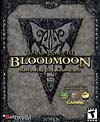
\includegraphics{media/image7.png}

{[}no fix{]} AllowWereWolfForceGreeting (is short variable)

Short AllowWereWolfForceGreeting

This variable allows to use ForceGreeting on a werewolf character. Used
on cariushuntscript, dulkscript, heartfanghuntscript. The variable
simply has to be declared, not set to a specific value.

\textbf{Example:}

\lstinputlisting{scripts/dulkScript.txt}

\hypertarget{multiple-choice-asking-questions}{%
\subsubsection{Multiple choice -- asking
questions}\label{multiple-choice-asking-questions}}

{[}no fix{]} Choice, ``choice 1'', choice1\_enum {[}"choice 2",
choice2\_enum, \ldots{]}

Choice "yes", 1, "No, certainly not!", 2

This is used in dialogue result fields to ask a decision of the player
or can be called just to "continue" a longer speech. After the PC makes
his choice, the same topic will be checked again, and you can provide
the correct response by using function / choice / = / choice\_enum in
the speaker conditions of the dialogue window. Choice can be used in
script, if the dialogue window is open. If the same resultbox/script
contains more than one choice call, the choices are presented to the
player as a single list (unlike MessageBoxes).

\hypertarget{section-11}{%
\subparagraph{}\label{section-11}}

The limit of choices per result or per call may well be version
dependent. It has been reported that there is a limit of 5 choices per
call, but I'm not sure which version this was tested with. Under version
1.6.1820, I don't think there's a limit on the number of choice
\emph{calls} in a single result, but only 20 choices can be displayed on
screen at one time: if more are displayed, the game will freeze when the
player clicks one (this applies to scripts as well as dialogue results).
More than 20 \emph{possible} choices won't cause problems as long as no
more than 20 are actually displayed (i.e. using conditional statements
to select 20 or less from a larger number of choices is OK).

On using Choice in script: I don't advise using it in a script that also
contains a StartScript command, as this can also freeze the game
sometimes. If you need to use both, you might try delaying the
StartScript part until out of menumode if possible or using some
condition to ensure that the choices can't be given more than once (not
tested).

\hypertarget{adding-to-the-journal-and-testing-journal-entries}{%
\subsubsection{Adding to the journal and testing journal
entries}\label{adding-to-the-journal-and-testing-journal-entries}}

{[}no fix{]} Journal, "Journal\_ID", Index\_enum

Journal, MG\_BCShroomsCombat, 10

This adds a journal entry to your in-game journal. The journal entry
must have previously been set up in the dialogue editor. Index
references which part of a journal topic is added. Beware of using
simple names for journal topics, adhere to Bethsoft's two letter
standard (see above example) -- otherwise the journal entry might show
up as a regular conversation response, just like any other, if the topic
title shows up in a conversation!

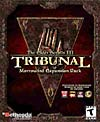
\includegraphics{media/image6.png}

{[}no fix{]} SetJournalIndex "Journal\_ID" index\_enum

SetJournalIndex "MG\_BCShroomsCombat" 99

SetJournalIndex will set the index to the specified value, whether or
not an entry exists for that index. This can be used to restart quests
or repeat sections (by setting the index backwards), or for temporary
storage of simple flags that don't need an own journal entry. However,
it should not be used to finish quests, as the quest will not be removed
from the active quests list (Journal does not have this problem, so it
is to be preferred for finishing quests).

\textbf{Note:} If the index set does not have a valid journal entry
(i.e. that index isn't defined in the "info" section of the dialogue
window), the value will be lost when a savegame is reloaded (the index
will revert to the last valid entry given). Therefore this can also be
used to detect if the player has reloaded the game:

if ( ( getjournalindex "dummy" ) != 100 )\\
Messagebox "You just reloaded, Cheater!!!"\\
setjournalindex "dummy" 100\\
endif

Where "dummy" is any journal topic that has no text for index 100.\\
\strut \\
The best thing is that it's most easy to use this in dialogue: Send the
player to the "test of courage", and set the journal index in
dialogue-result. When the player comes back, and the index differs, then
the player has failed the test. (Info on this function provided by JOG).

{[}no fix{]} ClearInfoActor

This is a function that is used in the results section of a dialogue
response -- using this function will stop the response from appearing in
the PC's journal (under "Topics"). Useful to avoid cluttering the topic
with useless information. Note however that if all responses for a topic
use ClearInfoActor, the topic will still appear in the topics list in
the journal, but clicking it will take the player to a blank page.

{[}no fix{]} GetJournalIndex, "JournalID" (returns short)

If ( GetJournalIndex, MG\_BCShroomsCombat == 10 )

This function returns the index of the current journal entry for that
journal topic (meaning the last index given, or the last index given for
which an entry exists in the case of SetJournalIndex and a reloaded
savegame). This is very convenient for keeping track of quest
advancement, and to have a script react according to what parts of the
quest have already been performed.

Sample Script: Here is a short script demonstrating the use of both
functions from the game:

\lstinputlisting{scripts/attack_slave.txt}

\hypertarget{special-dialogue-only-functions}{%
\subsubsection{Special dialogue-only
functions}\label{special-dialogue-only-functions}}

Among the functions available for defining dialogue conditions in the
dialogue editor there are a few that do not have a direct equivalent in
scripting functions. By using dialogue (e.g. using ForceGreeting,
voice-dialogue or strategically placed quest NPCs) and the dialogue
result field, you can still make use of these functions for scripting
purposes, e.g. by setting a global variable in the result field.
Examples of such functions are:

PC Sex (dialog)

This is 0 if the player is male and 1 if the player is female.

\textbf{Note:} This is the only known way to determine the player's sex.
You could use this to set a global variable that contains the Player's
gender - the most inconspicuous way would be to do this via voice
dialogue, e.g. one could put a silent hello greeting for all NPC's on
top of the list that sets a global variable "PC\_sex" to 1 when the
player is female, 2 when the player is male. The topic should be
filtered to only be active when PC\_sex equals 0.

Talked to PC (dialog)

This is 1 if the speaker has talked to the player and 0 otherwise. You
can use this to have someone say something the first time you speak with
them -- or for our scripting purposes to mark this person as "known" by
the player.

\textbf{Note:} The Talked to PC flag is subject to the "72-hours bug",
i.e. it will by default be reset if the NPC's cell has not been active
for 72 game hours or longer. See \emph{ForceGreeting} for specific
workarounds, and the "72-hours bug" section under "Tips and Tricks" for
more general information.

Rank Requirement (dialog)

Rank Requirement checks to see if you "qualify" for the next rank in the
speaker's faction.

\begin{itemize}
\item
  Returns 0 if you do not have enough Faction Reputation and do not meet
  the skill requirements.
\item
  Returns 1 if you meet the skill requirements, but do not have the
  Faction Reputation.
\item
  Returns 2 if you have the Faction Reputation, but do not meet the
  skill requirements.
\item
  Returns 3 if you qualify.
\end{itemize}

PC Clothing Modifier (dialog)

This is the total value of all the clothing and armor the player is
wearing. The value of your equipment changes the disposition of people
in the game.

Friend Hit (dialogue)

Used in dialogue for when you attack a member of your group (like a
follower)

The return values are:

0 = never been hit

1 = hit by pc 1st time

2 = hit by pc 2nd time

3 = hit by pc 3rd time

4 = hit by pc 4th time and the npc/creature is not in combat with the PC

Friend hit will reset if the player hits a different actor. It also
appears to reset if the actor starts combat, even if there are no hits
(I tried "ActorID-> StartCombat ActorID" - i.e. "start combat
with yourself" - in dialogue results, and this seemed to reset friend
hit).

\hypertarget{changing-the-hello-setting}{%
\subsubsection{Changing the Hello
setting}\label{changing-the-hello-setting}}

Get/Mod/SetHello

Changing this changes it for ALL references of the Actor. Some info from
the helpfile: Hello equates to the distance at which the Actor will
stop, face the PC and say hello. The setting (which defaults to 30) is
multiplied by the game setting, iGreetDistanceMultiplier, which defaults
to 7. Thus, a setting of 30 yields a hello distance of 210 (just under
10 feet).

\hypertarget{useful-dialogue-variables}{%
\subsubsection{Useful dialogue
variables}\label{useful-dialogue-variables}}

A number of short variables are used by Bethesda to block certain
dialogue. These must simply be declared in a script on the actor, no
value is required.

They are checked for using the Not Local filter as described in the
helpfile:

\begin{longtable}[]{@{}
  >{\raggedright\arraybackslash}p{(\columnwidth - 2\tabcolsep) * \real{0.14}}
  >{\raggedright\arraybackslash}p{(\columnwidth - 2\tabcolsep) * \real{0.86}}@{}}
\toprule
\begin{minipage}[b]{\linewidth}\raggedright
Nolore
\end{minipage} & \begin{minipage}[b]{\linewidth}\raggedright
Blocks most non-specific dialogue
\end{minipage} \\
\midrule
\endhead
NoIdle & Blocks Idle voice, used for vampires \\
NoFlee & Blocks flee voice, used for vampires \\
NoHello & Blocks Hello voice, used for vampires \\
\bottomrule
\end{longtable}

This is true if the speaker does not have this local variable. Unlike
most "Not" functions, this one does care what you set the variable to.
Both the dialogue and the variable itself should be set to 0. This can
be confusing. Here is a table of how this works:

\begin{longtable}[]{@{}
  >{\raggedright\arraybackslash}p{(\columnwidth - 6\tabcolsep) * \real{0.25}}
  >{\raggedright\arraybackslash}p{(\columnwidth - 6\tabcolsep) * \real{0.25}}
  >{\raggedright\arraybackslash}p{(\columnwidth - 6\tabcolsep) * \real{0.25}}
  >{\raggedright\arraybackslash}p{(\columnwidth - 6\tabcolsep) * \real{0.25}}@{}}
\toprule
\begin{minipage}[b]{\linewidth}\raggedright
Not Local
\end{minipage} & \begin{minipage}[b]{\linewidth}\raggedright
Variable Exists
\end{minipage} & \begin{minipage}[b]{\linewidth}\raggedright
Value
\end{minipage} & \begin{minipage}[b]{\linewidth}\raggedright
Pass?
\end{minipage} \\
\midrule
\endhead
(in dialogue) & (y/n) & (in the script) & (speaker will say this) \\
= 0 & No & NA & Yes \\
= 0 & Yes & 0 & No \\
= 0 & Yes & 5 & Yes \\
= 1 & No & NA & Yes \\
= -3 & Yes & -3 & No \\
\bottomrule
\end{longtable}

\hypertarget{changing-and-testing-skills-attributes-and-other-stats}{%
\section{\texorpdfstring{\hfill\break
Changing and testing Skills, Attributes, and other
Stats}{ Changing and testing Skills, Attributes, and other Stats}}\label{changing-and-testing-skills-attributes-and-other-stats}}

\hypertarget{get-set-and-modify-stats---general-remarks}{%
\subsection{Get, Set, and Modify stats - general
remarks}\label{get-set-and-modify-stats---general-remarks}}

Get\emph{Stat} (returns float)

Set\emph{Stat}, var\_float

Mod\emph{Stat}, var\_float

Set floatvar to ( Player-> GetHealth )

Player-> SetWillpower, 20

Player-> ModHealth, floatvar

This is really a whole family of functions that can alter player and
Actor stats, AI settings and more. Replace \emph{Stat} with any of the
game stats, attributes, AI-settings, resistances, reputation, etc.
(\textbf{list see Appendix}). Positive values are added to current stat,
negative values subtracted.

GetStat returns a float value with the \textbf{current} value of
\emph{Stat} (Not the maximum or base "natural" value of that stat for
the player, but what is currently used by the game, e.g. it could be
boosted by magic or reduced by disease).

Set\emph{Stat} sets the stat's \textbf{base and current} value to the
given value.

Mod\emph{Stat} adds (positive values are added to current stat, negative
values subtracted) the given value to both the \textbf{base and current}
value of \emph{Stat}. Mod\emph{Stat} can not set an attribute beyond its
natural limit (100) while Set\emph{Stat} can. Presumably the behavior is
equivalent for other \emph{Stat}'s.

\textbf{Note:} This is not true of some of the more unusual stats like
resistances, which can be negative (weakness) and aren't limited to 100
either.

There are so many things you can do with this set of functions that it
is not very useful to provide a sample script. Take a look at the
Marksman Toggle script in the Tips and Tricks section for a good
example. The script given under "Resurrecting a dead Actor" below also
uses ModHealth, as do many others.

These commands have a wealth of applications. They could be used for
special items, curses, blessings, to gain information on the player's
strengths and weaknesses, and to change AI settings (making an Actor
more aggressive after player has insulted him, making an NPC
uncommunicative at night etc.). Another popular use is to change weapon
stats to make NPC's switch their equipment.

\textbf{In the 8\textsuperscript{th} edition of this guide many of these
functions have been sorted into the appropriate chapters (e.g. magic,
combat, etc. )}

\hypertarget{determining-and-changing-actor-and-player-stats}{%
\subsection{\texorpdfstring{\hfill\break
Determining and changing Actor and player
stats:}{ Determining and changing Actor and player stats:}}\label{determining-and-changing-actor-and-player-stats}}

\hypertarget{determining-and-changing-attributes}{%
\subsubsection{Determining and changing
Attributes:}\label{determining-and-changing-attributes}}

\emph{Get/Mod/Set}Strength

\emph{Get/Mod/Set}Intelligence

\emph{Get/Mod/Set}Willpower

\emph{Get/Mod/Set}Agility

\emph{Get/Mod/Set}Speed

\emph{Get/Mod/Set}Endurance

\emph{Get/Mod/Set}Personality

\emph{Get/Mod/Set}Luck

\hypertarget{determining-and-changing-health-magicka-fatigue}{%
\subsubsection{Determining and changing Health, Magicka,
Fatigue:}\label{determining-and-changing-health-magicka-fatigue}}

\emph{Get/Mod/Set}Health

\emph{Get/Mod/Set}Magicka

\emph{Get/Mod/Set}Fatigue

These return, change or set the vital functions of the PC. For NPC and
the player the Get functions will report the current
health/magicka/fatigue. GetHealth also works on weapons / armor, but
only returns the maximum health. No function is known that reports
current item health (Forum info/Mana User).

\hypertarget{special-use-with-modstat-only}{%
\subparagraph{\texorpdfstring{Special use with Mod\emph{Stat}
only:}{Special use with ModStat only:}}\label{special-use-with-modstat-only}}

ModCurrentHealth, var\_float

ModCurrentMagicka, var\_float

ModCurrentFatigue, var\_float

While ModHealth changes both the maximum and the current health of an
Actor for the same amount (e.g. even a healthy Actor would be affected),
ModCurrentHealth affects only the current health and can not set health
above the original maximum health value for that Actor (so doing
ModCurrentHealth, 10000 to an Actor with 70 Health and a current health
of 35 would set Health to 70 -- Doing ModHealth, 10000 would set him to
10035 health).

\emph{Changing Health:}

SetHealth affects the object, not just a reference. If you use SetHealth
from a global script on a non-unique ID, it will apply to all instances
of the object that the player has not encountered yet (but if the player
has already encountered that reference, it won't be affected). If
SetHealth is used from a targeted script on a non-unique ID, it will
have much the same effect as a global script but will also affect the
script's target, even if the player has encountered it already.
ModCurrentHealth is the reverse: it affects the reference rather than
the object. SetHealth in the console window with a reference selected
will also affect only that reference.

Note that the same does not apply to other derived attributes: If you
place a new reference, Fatigue will be at editor level, and Magicka will
be auto-calculated from Intelligence (regardless of editor level).

GetHealthGetRatio (returns float)

This function returns the health ratio of the Actor as a float value
from 0 to 1, e.g. 1 means 100\% health, 0.9 means 90\% health and 0
means, well, dead I guess. This replaces the erroneously listed function
GetHealthRatio listed in the original helpfile.

If you want to know an Actors maximum health (Remember, GetHealth
returns your \emph{current} health points) you can use this:

Float MaxHealth

Float CurrentHealthRatio

Set CurrentHealthRatio to ( "Actor ID"-> GetHealthGetRatio )

if ( CurrentHealthRatio > 0 )

Set MaxHealth to ( ("Actor ID"-> GetHealth ) /
CurrentHealthRatio )

else

Set MaxHealth to 0

endif

\hypertarget{determining-and-changing-skills}{%
\subsubsection{Determining and changing
Skills:}\label{determining-and-changing-skills}}

Changing weapon skills can be used to change what weapon the NPC uses by
default. This doesn't appear to work correctly for armor -- the NPC will
only wear armor based on the skills set in the TES CS. If you know the
item ID, and have either Tribunal or Bloodmoon, you can use the Equip
function to force the NPC to use it (forum Info/Vorwoda\_the\_Black).
See the tips and tricks section for an example.

What's not obvious is the range of acceptable values for a skill: its
not just 0-100 as you might expect. In fact skills appear to be stored
as a float so you can set some large numbers in there, but there are
some checks: you can't set negative values, and decimal points are
discarded when saving/loading (Thanks FreshFish).

\emph{Get/Mod/Set}Block

\emph{Get/Mod/Set}Armorer

\emph{Get/Mod/Set}MediumArmor

\emph{Get/Mod/Set}HeavyArmor

\emph{Get/Mod/Set}BluntWeapon

\emph{Get/Mod/Set}LongBlade

\emph{Get/Mod/Set}Axe

\emph{Get/Mod/Set}Spear

\emph{Get/Mod/Set}Athletics

\emph{Get/Mod/Set}Enchant

\emph{Get/Mod/Set}Destruction

\emph{Get/Mod/Set}Alteration

\emph{Get/Mod/Set}Illusion

\emph{Get/Mod/Set}Conjuration

\emph{Get/Mod/Set}Mysticism

\emph{Get/Mod/Set}Restoration

\emph{Get/Mod/Set}Alchemy

\emph{Get/Mod/Set}Unarmored

\emph{Get/Mod/Set}Security

\emph{Get/Mod/Set}Sneak

\emph{Get/Mod/Set}Acrobatics

\emph{Get/Mod/Set}LightArmor

\emph{Get/Mod/Set}ShortBlade

\emph{Get/Mod/Set}Marksman

\emph{Get/Mod/Set}Mercantile

\emph{Get/Mod/Set}Speechcraft

\emph{Get/Mod/Set}HandToHand

\hypertarget{determining-and-changing-level}{%
\subsubsection{Determining and changing
Level}\label{determining-and-changing-level}}

\emph{Get/Mod/Set}Level (only works with Set and Get)

Sets the Actors level, and only that. Skills and stats are not
automatically increased, nor does the levelling menu come up when you
call this for the player.

Note that SetLevel does not accept variables (using variables will not
generate an error, but the actor's level will be set to 0).

\hypertarget{getstat-modstat-and-setstat-a-concerned-modders-guide.---galsiah}{%
\subsubsection{GetStat, ModStat and SetStat: A concerned modder's guide.
-
Galsiah}\label{getstat-modstat-and-setstat-a-concerned-modders-guide.---galsiah}}

\emph{\textbf{Throughout the term ``base stat'' means the value of the
stat when yellow -- i.e. unmodified by any in game bonus / penalty apart
from fortification abilities.}}

\hypertarget{getstat}{%
\subparagraph{GetStat:}\label{getstat}}

Always returns the current stat -- including any bonus / penalty. No
nasty side effects as far as I'm aware, so GetStating should always be
safe. There is (sadly) no GetBaseStat function. MWSE has these, but they
don't include e.g. racial fortification abilities in the base, and
usually you'd want them included.

Most of the problems of ModStat and SetStat explained below are only
really important for the player (and possibly companions). These
functions won't do anything worse than screwing up the stats they
operate on, so for normal NPCs, there's not much point worrying about
all this.

As with pretty much anything in Morrowind modding, if you have a choice
to use scripting or something else, then use something else. For ModStat
/ SetStat, the ``something else'' will usually be fortify/drain stat
spell effects or curses. For most purposes, standard effects will work
as well as ModStat and SetStat, and will be much less buggy.

\hypertarget{modstat}{%
\subparagraph{ModStat:}\label{modstat}}

Usually increases (or decreases) the stat concerned by the amount given
Both the current stat and the base stat are affected. Usually preserves
the amount of fortification or damage on the stat.

E.g. for a player with strength 50(base) + 10(fortification) =
60(current)

Player-> ModStrength 10 will give 60(b.) + 10(f.) = 70(c.),
just as you'd expect.

Limitations: ModStat can never decrease a stat below zero. It also
cannot increase a base stat to a value over 100. Trying to Modstat below
zero or above 100 can cause trouble in the following ways:

Strength = 30(b.) + 0(f.) = 30(c.)

ModStrength, -50 gives

Strength = 0(b.) + 0(f.) = 0(c.)

ModStrength 50 {[}hoping to undo the first modstrength{]}

Strength = 50(b.) + 0(f.) = 50(c.) -- and the player has a permanent
bonus.

You can try to avoid this by instead checking that you don't reduce the
stat by more than the current value, but that won't always work. For
example:

Strength = 40(b.) + 10(f.) = 50(c.)

ModStrength -50

Strength = 0(b.) + 0(f.) = 0(c.)

ModStrength 50

Strength = 50(b.) + 0(f.) = 50(c.) -- and the player's base strength is
increased.

If he then removes the fortification, his strength will show up as
damaged. Restoring and replacing the fortification will leave him with:

Strength = 50(b.) + 10(f.) = 60(c.)

It's never safe to ModStat down by more than the player's base stat.
Given that there's no failsafe method to determine the player's base
stat, this is annoying {[}the only ways I know to determine the player's
base stat are the method which I use in GCD -- complicated, and doesn't
work correctly when the player's stat is damaged -, using MWSE, which I
think doesn't include permanent abilities in the base (for most purposes
you'd want permanent abilities to count towards the base). Even
systematically removing every conceivable bonus / penalty -- which is a
drag anyway -- won't always work with other scripted mods{]}.

Going over 100 has similar problems. The following is fine:

Strength = 70(b.) + 20(f.) = 90(c.)

ModStrength, 20 gives

Strength = 90(b.) + 20(f.) = 110(c.)

ModStrength -20 gives

Strength = 70(b.) + 20(f.) = 90(c.) -- all fine.

However, this also happens for some reason:

Strength = 70(b.) + 20(f.) = 90(c.)

ModStrength, 50 gives

Strength = 100(b.) + 40(f.) = 140(c.) -- already screwed up.

ModStrength -50 gives

Strength = 50(b.) + 40(f.) = 90(c.) -- further screwed up.

This problem arises because if a stat is fortified or damaged, and the
base is not 100, ModStat always increases the current stat by the value
you give it, even if the base stops at 100. If the base is 100,
ModStating won't have any effect. If the stat is equal to its base
value, ModStat will behave normally.

So this is fine (so long as you don't ModStat -50 afterwards):

Strength = 70(b.) + 0(f.) = 70(c.)

ModStrength, 50 gives

Strength = 100(b.) + 0(f.) = 100(c.)

And this is fine:

Strength = 100(b.) + 20(f.) = 120(c.)

ModStrength, 50 gives

Strength = 100(b.) + 20(f.) = 120(c.)

But this isn't:

Strength = 99(b.) + 20(f.) = 119(c.)

ModStrength, 50 gives

Strength = 100(b.) + 69(f.) = 169(c.) -- oh dear.

Of course as a modder you won't know in general what the Base +
Fortification is before you use the ModStat function, so you have no way
to compensate for errors even once you know what can go wrong. Joy!

Ok, so as long as you never try to ModStat the current stat over 100,
everything should be fine, right?

Sadly not:

Strength = 95(b.) - 10(damage) = 85(c.)

ModStrength, 15 gives

Strength = 100(b.) + 0(f.) = 100(c.) -- OK so far

ModStrength, -15 gives

Strength = 85(b.) + 0(f.) = 85(c.) -- Permanent strength damage.

So under what circumstances will ModStating up or down give reliably
predictable results?

Only when you know the base value of the stat.

\hypertarget{can-you-reliably-work-out-the-base-value-of-the-stat}{%
\subparagraph{Can you reliably work out the base value of the
stat?}\label{can-you-reliably-work-out-the-base-value-of-the-stat}}

No -- only in some situations is it possible (the process is explained
below, and implemented in my Gals\_Sk\_Acrobatics script in GCD). Even
then it's not easy. (it's worth checking script extenders for updates
though)

\hypertarget{setstat}{%
\subparagraph{SetStat:}\label{setstat}}

Sets both the base and the current value to the value you give it (also
accepts local variables). Can set base and current to values over 100.
Accepts negative values, which can be useful in conjunction with ModStat
(see below).

This will pretty much always cause problems if the player's current stat
is not equal to their base stat. If their stat is fortified, and you
SetStat it, it'll turn yellow at the value you give it. Removing the
fortification, then restoring will give the player a permanent bonus.\\
If their stat is damaged, SetStating it will again turn it yellow, but
this time at a lower value than you (probably) intended. They will
instantly have their base knocked down to the value you set.

Using SetStat is therefore never even slightly safe unless you know the
player's base stat, and compensate accordingly. While you can't
guarantee that ModStat won't cause trouble, you can almost guarantee
that SetStat will.

Using SetStat is therefore almost always a bad decision -- if you're
ever not sure whether it's a bad decision, then it is.

\hypertarget{then-are-these-functions-useless}{%
\subparagraph{Then are these functions
useless!?}\label{then-are-these-functions-useless}}

Not always. You can use them on NPCs without worrying too much. Using
them on companions could occasionally not have the effect you want, but
it's unlikely the player would notice.

Using ModStat on the player can be safe, so long as you're careful --
e.g. to increase strength by (up to) 10 points temporarily, you could:

Give the player a very strong restore strength curse for a frame or two.
(you can then be sure his strength isn't damaged)

ModStrength by MIN\{ 10, 100-current \}

\ldots{}

ModStrength down by the same amount when you want the effect to finish.

You can never be sure that giving a temporary penalty won't cause
trouble, but if you only reduce the stat by at most 30, then it'll
usually be fine since most players start with all stats that high.
Restoring the stat after you've reduced it like this could cause trouble
if the player has since gained base stat points, and his stat started
close to 100.

\hypertarget{some-cunning-tricks-with-setstat-modstat}{%
\subparagraph{\texorpdfstring{\hfill\break
Some "cunning" tricks with SetStat /
ModStat:}{ Some "cunning" tricks with SetStat / ModStat:}}\label{some-cunning-tricks-with-setstat-modstat}}

Warning: using the following tricks might cause even more trouble than
using the functions normally. Use with care. Conflicts are likely.

\hypertarget{finding-the-base-of-a-stat}{%
\subparagraph{Finding the base of a
stat:}\label{finding-the-base-of-a-stat}}

You can find the base of a stat using the (mis)behaviour of ModStat, as
follows:

(1)Make sure that the player's stat isn't damaged {[}You have been
tracking increases in the natural values of the stat since the beginning
of the game, haven't you? If you haven't, then you have no way of
knowing if it's damaged -- you could check the base value on
installation of your mod, so long as you ask the player to install when
stats aren't damaged / fortified{]}.

(2)If it is damaged, give up. (you might want to check script extenders)

(3)If it isn't:

(4)Store the current value of the stat.

(5)Mod the stat up to 100 if it isn't already 100 or more.

(6)ModStat, 1 as many times as you can while the stat still increases.

(7)The fortified part of the stat is the value it reached minus 100.

(8)The base part of the stat is the current value minus the fortified
part.

(9)Return the stat to its current value (DON'T use SetStat, use
ModStat).

Armed with the base value, you can now use ModStat and SetStat wisely
and safely, so long as you're very careful.

\hypertarget{damaging-a-stat}{%
\subparagraph{Damaging a stat:}\label{damaging-a-stat}}

To set a stat to e.g. 50 damaged from 70, you can do the following:

Player-> SetStat, -20 {[}Base and current are now both -20{]}

Player-> ModStat, 0 {[}Necessary: sets the base to 0{]}

Player-> ModStat, 70 {[}Base = 70, current = 50 (red){]}

This level of precision is not possible in general using e.g. damage
stat curse effects, but it's not usually necessary either. The above can
also be done within one frame, whereas a curse effect might take a
second to kick in. Again, the speed can be useful, but is usually
unnecessary.

\textbf{Fortifying a stat:}

To set a stat to e.g. 120 fortified from 90, you can do the following:

Player-> SetStat 130 {[}Base and current are now both 130{]}

Player-> ModStat, 0 {[}Necessary: sets the base to 100{]}

Player-> ModStat, -10 {[}Base = 90, current = 120 (white){]}

\hypertarget{combat}{%
\section{Combat}\label{combat}}

\hypertarget{initiating-and-ending-combat}{%
\subsection{Initiating and ending
combat}\label{initiating-and-ending-combat}}

StartCombat, "ActorID"

StopCombat

"Actor\_ID1"-> StartCombat, "ActorID2"

"Actor\_ID1"-> StopCombat

StartCombat and StopCombat are used to set an Actor into combat mode or
back into normal mode. Start combat will make the calling Actor attack
the Actor supplied as the argument. While StopCombat seems to be "safe"
to use "every frame", you should supply a do once condition of some sort
when issuing the StartCombat command, otherwise the Actor might not do
anything. Nevertheless continuous StopCombat is very dangerous to use,
because it makes the NPC completely helpless: it will not retaliate when
attacked (which however allows you to create a real pacifist\ldots).
Another caution regarding StopCombat is that it stops combat for
\textbf{all} actors involved, other than the player.

Once in combat mode the AI settings of the Actor apply normally, e.g. if
the Actor has a high flee setting, he will flee despite the StartCombat
command. For this reason, you will often see that the Fight rating is
also changed when initiating combat in many scripts:

If ( GetDeadCount, "My Friend" > 0 )

\textbf{StartCombat}, Player

\textbf{SetFight}, 100

endif

The same applies to StopCombat: if the actor has a high Fight rating he
will go briefly into an idle stance (sheathe weapon or un-ready spell),
then quickly enter combat with the player again; to stop combat
completely, set the actor's Fight rating to a low value as well.

\hypertarget{detecting-attack}{%
\subsection{Detecting Attack}\label{detecting-attack}}

{[}no fix{]} OnPCHitMe (is local short variable)

Short OnPCHitMe

If ( OnPCHitme == 1 )

A local game variable (not a function, you must declare it as a variable
as shown above) that gets set to 1 when the player hits the calling
Actor. Must be manually reset. It seems the use of the variable
"short-circuits" normal NPC behavior in that an NPC with a script that
uses this variable will not attack on its own accord. If you don't want
the Actor to remain passive you have to manually \emph{StartCombat} (see
example below). Once the Actor is in combat mode, \emph{OnPCHitMe} does
not report any further hits by the PC. Except, according to information
on the forum, \emph{OnPCHitMe} gets reset (to 0) if another Actor hits
the calling Actor after the PC did, then the variable gets reset to 1 if
the player hits again.

\textbf{Note:} According to info provided by Nigedo, OnPCHitMe also
registers if the PC commits a crime, and the Actor has a sufficiently
high alarm setting.

Example Script: An example from my traveling merchants mod, to make a
guar handler defend his charge while not in AIFollow mode, I attached
this to the guar:

\lstinputlisting{scripts/_HB_Adros_GuarDefend.txt}

GetAttacked (returns Boolean/short)

If ( Actor-> GetAttacked == 1 )

Returns 0 if the Actor has never been attacked and 1 if he has ever been
attacked.

\textbf{Example script:} Uupse protects Yagrum Bagarn:

\lstinputlisting{scripts/uupse_Bagrum.txt}

GetTarget, "Actor ID" (returns Boolean/short)

If ( Actor-> GetTarget, Player == 1 )

GetTarget tests to see if the target is in focus. For the player, it's
the test to see if the target is currently in the crosshair and can be
activated. Of course NPCs don't have a crosshair like the player, but
they get the same logic. (Thanks to cdcooley for the explanation)

If you want to use GetTarget to see if one actor is fighting another,
you would have to combine it with GetWeaponDrawn and GetSpellReadied.

short temp\\
set temp to GetWeaponDrawn\\
set temp to ( temp + GetSpellReadied )\\
if ( temp > 0 )\\
\hspace*{0.333em}\hspace*{0.333em}\hspace*{0.333em}\hspace*{0.333em}if (
\textbf{GetTarget}, Player == 1 )\\
\hspace*{0.333em}\hspace*{0.333em}\hspace*{0.333em}\hspace*{0.333em}\hspace*{0.333em}\hspace*{0.333em}
; In combat with the player here\\
\hspace*{0.333em}\hspace*{0.333em}\hspace*{0.333em}\hspace*{0.333em}endif\\
endif

HitOnMe, "Weapon ID" (returns Boolean/short)

HitAttemptOnMe, "Weapon ID" (returns Boolean/short)

These functions return true (1) for 1 frame if the calling Actor is
successfully hit or if it was attempted to hit it with a specified
weapon. HitOnMe is used only in the LorkhanHeart script (only look at
that if you have finished the game or don't mind severe spoilers). I
guess it could be a nice function to script any kind of fight of the
"you need this special weapon to kill this particular monster" type.

\hypertarget{combat-related-getmodset-ai-functions-fight-flee-alarm}{%
\subsection{Combat related Get/Mod/Set AI functions: Fight, Flee,
Alarm}\label{combat-related-getmodset-ai-functions-fight-flee-alarm}}

\emph{Get/Mod/Set}Fight

Some info from the helpfile:

An Actor's fight setting determines how prone the Actor is to attacking
the PC. Mod/Set Fight appear to also affect all new references of the
actor you may add after calling this function (i.e. it affects the
object, not just a reference). When an Actor's fight setting hits 100,
they will attack the PC.

Player actions will increase (or decrease) an Actor's fight setting.
These are:

\emph{Get/Mod/Set}Flee

Changing this changes it for ALL references of the Actor (see note).

Setting this to a higher value will make the Actor more likely to flee,
but this may not always be the result, as the Actor will also use other
factors like how much damage they can give out, or other strategies they
may use such as magic and ranged combat. The behavior is strongly
influenced by a number of GameSettings that are listed below, and a
number of mods (e.g. by wakim and maxpublic) have tweaked these values
to allow for more realistic fleeing behavior.

\emph{Get/Mod/Set}Alarm

Changing this changes it for ALL references of the Actor (see note).

Some info from the helpfile: When a crime is committed, and it is
detected by an NPC, they will shout something at the player, this also
notifies other NPCs in the area.

When the NPCs hear this, they adjust their settings based on their alarm
setting. The higher the alarm setting, the angrier they will get.

If an NPC has an alarm of 100, he will put gold on the PC's head if they
hear of a crime.

If the NPC with alarm 100 is also of class ``Guard'', they will have
extra behavior:

Intercept the PC, by running up and arresting the PC.

If the PC's CrimeLevel is over 10000, they will attack on sight, instead
of initiating dialogue.

Guards will also attack any creatures they can see that are attacking
people (including the PC). If the player has followers (companions or
other NPCs in AIFollow mode), the presence of a guard-class NPC in the
party may also cause the non-guard followers to attack hostile creatures
before blows have been exchanged (normally a non-guard follower would do
nothing until a hit has occurred). -(Forum info/Neko)

\textbf{Note:} When you use these functions to alter the settings for an
actor, it alters the current reference of the actor AND the definition
of the actor. What this means is if you encounter a new actor of that id
that you haven't yet met, he will have the new alarm/Fight setting.
Also, if you leave the cell where an actor still has the old value, rest
for 3 days (to disconnect them from memory) then re-enter the cell, he
will take his value from the definition of the actor i.e. the new alarm
setting (Forum info / Cortex).

\hypertarget{keeping-track-of-kills-and-knockouts}{%
\subsection{Keeping track of kills and
knockouts}\label{keeping-track-of-kills-and-knockouts}}

OnDeath (returns Boolean/short)

If ( Actor-> OnDeath == 1 )

Returns 1 for 1 frame when the Actor is killed. OnDeath seems to reset
itself once it is used. This also means that only one script can
reliably detect death this way: if you have both a global and a local
script using this function, only the global script will detect OnDeath.
An alternative would be to use the GetHealth function. In the following
script only the first message box will be displayed (forum info /
Argent, ThePal):

\lstinputlisting{scripts/personScript.txt}

OnMurder (returns Boolean/short)

If ( Actor-> OnMurder == 1 )

Returns 1 for 1 frame when the Actor is murdered. The conditions for
\emph{OnMurder} are not entirely clear to me -- from the context of its
use in the game however, it seems that \emph{OnMurder} gets set when you
are reported as a murderer to the law ("your crime has been reported").
So a murder only happens when you kill someone illegally AND are seen.

\textbf{Sample Script:} this sets a variable that is used in the
"Redoran Hortator" dialogue topic to determine if the player has killed
a councilor:

\lstinputlisting{scripts/RedoranCouncilor.txt}

OnKnockout (returns Boolean/short)

If ( Actor-> OnKnockout == 1 )

Returns true for one frame when the Actor is knocked unconscious (e.g.
in hand-to-hand combat)

{[}no fix{]} GetDeadCount, "Actor ID" (returns short)

If ( GetDeadCount "divayth fyr" > 0)

The function returns the number of references (individuals) of type
"Actor ID" that have been killed. A useful function for quest scripting
to keep track of which NPCs are still alive. Note that there is an
equivalent function for dialogue as well. Other uses are imaginable,
e.g. building a reputation with certain monsters that might flee you
instead of fighting after you killed more than 100 of them, etc.

Sample Script:

GetDeadCount is often used to check if a certain NPC is dead. It is
advisable to use "> 0" in such cases, as you never know if
another mod might add another instance of that ID, so it's better to
play it safe.

\lstinputlisting{scripts/araraUvulasScript.txt}

\hypertarget{resurrecting-a-dead-actor}{%
\subsection{\texorpdfstring{\hfill\break
Resurrecting a dead
Actor}{ Resurrecting a dead Actor}}\label{resurrecting-a-dead-actor}}

Resurrect

gateway\_haunt-> Resurrect

This function brings an Actor back to life. His stats and inventory will
be reset, basically he "respawns". There is a bug when you use this
function on the player -- it will stop the PC (and all Actors) from
casting magic. After saving and reloading this side effect goes away.

\textbf{Note:} The Puzzle Canal Script shows an alternative: it simply
uses GetHealth <10 to determine when player is "nearly" dead and
then "resurrects" him by giving him his health back -- so the player
actually never really dies.

\textbf{Sample Script:} some people are just tougher than others\ldots{}

\lstinputlisting{scripts/dandrasScript.txt}

\hypertarget{crime}{%
\section{\texorpdfstring{\hfill\break
Crime}{ Crime}}\label{crime}}

\hypertarget{determining-and-changing-crime-level}{%
\subsection{Determining and changing Crime
Level}\label{determining-and-changing-crime-level}}

\emph{Get/Mod/Set}PCCrimeLevel (PC Only)

\emph{PCCrimeLevel} governs the gold you have to pay to be cleaned of
crimes, influences NPC disposition and how guards react to you. See also
the PayFine function.

\hypertarget{jailing-the-pc}{%
\subsection{Jailing the PC}\label{jailing-the-pc}}

{[}no fix?{]} GotoJail

Sends the PC to the (closest available) prison, more exactly speaking to
a PrisonMarker (Door object) and applies the usual prison penalties.

SampleScript:

Here is a cool little scripted item by B from the Modern Adventurer mod.
The cursed Holiday Pants that send you to prison:

\lstinputlisting{scripts/Holiday_script.txt}

\hypertarget{clearing-the-pc-of-crime}{%
\subsection{Clearing the PC of crime}\label{clearing-the-pc-of-crime}}

{[}no fix{]} PayFine

The PayFine function removes the stolen items from the PCs inventory; it
does not remove any gold. Call after paying a crime fee to clean AI.
Also puts the PCs hands down (that is not ready to cast or fight).

{[}no fix{]} PayFineThief

Like PayFine function but \emph{does not} remove stolen items from the
PCs inventory. Call to "clean AI". May have incorrectly removed stolen
items before one of the patches.

For examples check below, under "Useful global variables"

\hypertarget{detecting-crime}{%
\subsection{Detecting crime}\label{detecting-crime}}

{[}no fix{]} GetPCCrimeLevel (returns short)

Reports the current crime level of the PC. Can be used to detect whether
a crime the PC has committed has been seen. See the
"Bill\_MT\_writxxxxx" scripts for examples of its use.

An alternative was reported by Nigedo:

OnPCHitMe

If you declare OnPCHitMe in an NPC's script, any crime that they are
aware of causes this function/variable to return True. The crime does
not actually have to be committed against that NPC, they just have to
have a high enough Alarm setting to care about a crime being committed
within range, and the crime will count as a melee hit on them of zero
damage.

Although this makes OnPCHitMe less reliable for detecting just attacks
on the NPC it is declared on (I had to use a different method for the
script I was actually working on), it is potentially useful for
detecting crimes taking place.

It is possible to use this to detect all crime events in one script,
without needing an NPC to "report" them, i.e. increase Player's bounty,
or needing to check or adjust PCCrimeLevel.

I found that the following alarm settings will (usually) cause OnPCHitMe
to return True for the these events:-

\textbf{Event Minimum Alarm}

Any theft 10

Assault of an NPC 90

Murder of an NPC 10

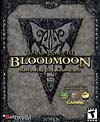
\includegraphics{media/image7.png}

{[}no fix{]} GetPCInJail (returns Boolean/short)

Bloodmoon adds a function that can be checked to see if the PC is in
Jail. The function will return 1 if traveling/in jail, zero otherwise.
This is used in the werewolf change script to stop the PC from changing
if either of these states are the case.

\textbf{Sample script:}

if ( PCWerewolf != 1 ) ; DON' RUN IF PLAYER ISN'T WEREWOLF

return

endif

if ( \textbf{GetPCinJail} == 1 )

return

endif

if ( \textbf{GetPCTraveling} == 1 )

return

endif

\hypertarget{useful-global-variables}{%
\subsection{\texorpdfstring{\hfill\break
Useful global
variables}{ Useful global variables}}\label{useful-global-variables}}

CrimeGoldDiscount (is global short)

Contains the amount of gold needed to pay the reduced fine at the
thieves guild.

CrimeGoldTurnIn (is global short)

Contains the reduced fee you have to pay when you turn yourself in.

PCHasCrimeGold (is global short)

Used in dialogue conditions. Gets set to 1 if player has enough gold to
pay for his crimes.

PCHasGoldDiscount (is global short)

Used in dialogue conditions. Gets set to 1 if player has enough gold to
pay thieves guild discount on the "price on your head".

PCHasGoldTurnIn (is global short)

Used in dialogue conditions. Gets set to 1 if player has enough gold to
the reduced crime fee that is charged when turning yourself in.

\textbf{Example:} A \textbf{dialogue result field} for the topic "price
on your head", for paying a fine at the thieves guild:

Player-> RemoveItem Gold\_001 \textbf{CrimeGoldDiscount}

\textbf{SetPCCrimeLevel} 0

\textbf{PayFineThief}

For comparison, this is the result fields that guards use when you have
a price on your head and turn yourself in (you find this under Greeting
0):

Player-> RemoveItem Gold\_001 \textbf{CrimeGoldTurnIn}

\textbf{SetPCCrimeLevel} 0

\textbf{PayFine}

Or if you get caught and have to pay the normal "fines and
compensation":

Player-> RemoveItem Gold\_001 \textbf{GetPCCrimeLevel}

\textbf{SetPCCrimeLevel} 0

\textbf{PayFine}

\hypertarget{magic}{%
\section{\texorpdfstring{\hfill\break
Magic}{ Magic}}\label{magic}}

\hypertarget{limiting-the-use-of-teleport}{%
\subsection{Limiting the use of
teleport}\label{limiting-the-use-of-teleport}}

{[}no fix{]} DisableTeleporting

{[}no fix{]} EnableTeleporting

Rather self explanatory, these functions turn the ability to use
teleporting magic on or off. Nice to keep those magic user types from
wimping out of your dungeon . In the original game it's only used when
the player encounters Dagoth Ur.

I won't show the whole script as it would be quite a spoiler, but here
is the part that uses the function:

short teleportDisabled

if ( teleportDisabled == 0 )

\textbf{DisableTeleporting}

Set teleportDisabled to 1

endif

This is later reset in the EndGame script.

\textbf{Note:} when the original Tribunal is installed this function is
effectively broken: One of the start-up scripts in Tribunal overrides
all other teleport commands and forces teleporting on except within one
specific area in Mournhold (thanks to Slink and Riiak for the info).
Here is the culprit:

\lstinputlisting{scripts/TribunalMain01.txt}

With one of the updates this problem was fixed. The latest version of
the script looks like this:

\lstinputlisting{scripts/TribunalMain02.txt}

Note: DisableTeleporting does not disable scripted amulets etc. for
teleporting. DinkumThinkum suggested the following workaround which uses
GetPCCell to check the player's current location. As long as they're in
one of the mod cells, nothing happens. If they're \emph{not} where
they're supposed to be, then the script teleports them back into the
correct area: back to the initial entry point for the mod, for example.
This wouldn't be exactly the same as blocking the teleports, but it
should make the area totally inescapable until you've fulfilled the
modder's conditions for getting out legitimately.

\lstinputlisting{scripts/DT_Test_BalmoraTrap.txt}

\hypertarget{limiting-the-use-of-levitation}{%
\subsection{Limiting the use of
levitation}\label{limiting-the-use-of-levitation}}

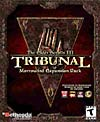
\includegraphics{media/image6.png}

{[}no fix{]} EnableLevitation

{[}no fix{]} DisableLevitation

These functions are used to allow and block Levitation magic effects.
When DisableLevitation is called, all existing Levitation effects are
canceled. When the player tries to cast a spell with a Levitate effect
while Levitation is disabled, a notify message is displayed with the
text in the GameSetting sLevitateDisabled. Currently this text reads
``Levitation magic does not work here.''

Sample scripts:

This script is on an object in the room with levitation disabled.

\lstinputlisting{scripts/clampstone.txt}

This script is on a door leaving the room.

\lstinputlisting{scripts/enable_lev_on_exit.txt}

\hypertarget{checking-and-managing-souls-and-soulgems}{%
\subsection{Checking and managing souls and
soulgems}\label{checking-and-managing-souls-and-soulgems}}

HasSoulgem, "CreatureID"

If ( Actor-> HasSoulGem, "golden saint" )

This function checks if the player has a soul gem containing the
specified soul in his inventory. A little used function that could allow
some fun quests and new uses for soulgems.

\textbf{Sample:} This is part of the StrongSoulCheck script:

if ( Player->\textbf{HasSoulGem} "atronach\_storm"
> 1 )

Set counter to ( counter + 2 )

elseif ( Player->\textbf{HasSoulGem} "atronach\_storm"
> 0 )

Set counter to ( counter + 1 )

endif

RemoveSoulgem, "CreatureID", number\_enum

Actor-> RemoveSoulGem, "golden saint", 1

Removes a soulgem with the specified soul from the players inventory.

Sample: this is the complementary part from RemoveStrongSoul script to
the example above:

if ( counter > 0 )

if ( Player-> HasSoulGem "atronach\_storm" > 0 )

Player->\textbf{RemoveSoulGem} "atronach\_storm" 1

Set counter to ( counter - 1 )

endif

endif

Note, the player will not be happy if they get Azura's Star taken away
by this. Here's a sample solution:

short StarCount ;They could have more than one I guess.

if ( OnActivate )

if ( Player->\textbf{HasSoulGem} "Golden Saint"
> 0 )

set StarCount to ( Player-> GetItemCount
"Misc\_Soulgem\_Azura" )

Player-> RemoveSoulGem "Golden Saint" 1

if ( ( Player-> GetItemCount "Misc\_Soulgem\_Azura" )
< StarCount )

Player-> AddItem "Misc\_Soulgem\_Azura" 1

endif

Player-> AddItem Gold\_001, 10000

MessageBox "Thank You, Come Again."

else

MessageBox "You have no Golden Saint souls."

endif

endif

AddSoulGem "creature ID", "soulgem ID"

AddSoulGem "atronach\_storm", Misc\_Soulgem\_Grand

AddSoulGem adds a soulgem of the specified type and with the specified
soul to the players inventory. You can't add more than one at a time
with this (giving it a count won't cause any problems, it's just
ignored).

DropSoulgem, "Creature ID"

DropSoulGem "atronach\_storm"

As far as I can tell, this function is broken (crashes the game).

{[}no fix{]} OnPCSoulGemUse (is short variable)

The Object is a soulgem and it has been used in either recharging or
item making

The soul gems in the game have the following ID's:

Soul Gem ID's:

Misc\_SoulGem\_Azura

Misc\_SoulGem\_Grand

Misc\_SoulGem\_Greater

Misc\_SoulGem\_Common

Misc\_SoulGem\_Lesser

Misc\_SoulGem\_Petty

This function was not used in the original game.

\hypertarget{adding-and-removing-spells-and-cursing}{%
\subsection{\texorpdfstring{\hfill\break
Adding and removing spells and cursing
}{ Adding and removing spells and cursing }}\label{adding-and-removing-spells-and-cursing}}

AddSpell, "SpellID"

RemoveSpell, "SpellID"

"Actor\_ID"-> AddSpell "Absorb Speed"

The AddSpell function will add the spell to the calling object. This can
mean two things: normal spells are added to the actor's spell list.
Curses, diseases etc, however will affect the calling object. The same
is true for the RemoveSpell function: Normal spells are removed from the
list, curses or diseases are removed as effects.

\textbf{Note:}

When you add a spell to a generic NPC, it is added to all NPCs of that
ID - unlike items, which are just added to the one NPC.

\hypertarget{some-general-notes}{%
\subparagraph{Some general notes:}\label{some-general-notes}}

You can not remove racial abilities with the RemoveSpell function (forum
info). You can remove birthsign abilities, but if the ability was added
by the player's birthsign (i.e. during character generation, not later
by script), the ability cannot be re-added afterwards (forum info /
Rocket).

(Mainly relevant for companions:) Any type of constant magical effect
(e.g. abilities, CE enchanted items, etc) on an NPC is reapplied when
the NPC changes cells, and when it gets high enough it "wraps around"
and usually starts working in reverse. Much of the time this is not
noticeable, but if necessary the problem can be avoided by removing and
re-adding the effect on CellChanged. In the case of some effects, e.g.
water breathing, the game may remove the effect too many times: in this
case SetWaterBreathing can be used (note that it must be reset after 72
game hours). (Forum info / CdCooley).

Abilities may sometimes not work as expected. If an ability is removed
by script, it may sometimes reappear after reloading a save, or later in
the game. Effects on the character's stats may also reappear or not be
removed properly on occasion (forum info / exclusiveor77). The other
problem with abilities is that damage abilities do permanent damage
(i.e. a damage health ability damages maximum health: curses do not have
this problem). This does not seem to be true of drain or fortify
effects, where it would make a lot more sense. (Forum info / ManaUser)

Curses do, however, have the problem that they can be removed by "Remove
Curse" spells.

On the Remove Curse effect, in my tests it worked but somewhat
strangely. It's percentile (like dispel rather than cure paralysis) but
the percent seemed to be cumulative or something. For example a 1\%
remove curse spell never worked (as many times as I tested it) unless I
first cast something like a 100\% remove curse spell. -(ManaUser)

\hypertarget{casting-spells}{%
\subsection{\texorpdfstring{\hfill\break
Casting spells}{ Casting spells}}\label{casting-spells}}

Cast, SpellID, "TargetID"

Object\_ID-> Cast, "flame", Player

The Cast function makes the calling object cast the spell "SpellID" on
the target "TargetID", and Target will suffer or benefit from the
effects normally. The calling object does not need to have the spell in
inventory: it will be cast regardless.

The spell's target must be specified, even if the spell is "on self". In
this case you can specify the caster or the player as the target: if the
spell is "on self" it won't make any difference. If you intend to place
the target during the game, you will still need to place a reference in
the editor. Cast will prefer a reference in the current cell if there is
one available, so there's no need to move a reference from a storage
cell: you can just place a new one.

\hypertarget{notes}{%
\subparagraph{Notes:}\label{notes}}

\begin{itemize}
\item
  \begin{quote}
  It was believed that Cast would only work on the PC. At least with
  Tribunal (not sure about earlier versions) you can use cast to cast a
  spell from an activator, or any other object, on an Actor. However,
  make sure the object you are casting the spell from is not in the
  inventory of another actor/object, as that will result in a CTD.
  \end{quote}
\item
  \begin{quote}
  You cannot force an actor to cast a spell on an activator, but you can
  have them cast on themselves, other actors, or the player.
  \end{quote}
\item
  \begin{quote}
  You can get non actor objects to cast spells on themselves. Just use
  the player (or some other object) as a target, but cast an ``On Self''
  spell.
  \end{quote}
\item
  \begin{quote}
  NPCs will not automatically lose magicka from a scripted cast. If you
  want the NPC to use up magicka in casting, this also needs to be
  scripted. -(Forum info/Kateri)
  \end{quote}
\item
  \begin{quote}
  If the spell's target is not in the current cell, the NPC will cast
  anyway (this doesn't cause any errors, but it does look a little odd -
  particularly targeted spells). They will also cast 'through' objects,
  other NPCs, walls\ldots{} anything that's in the way.
  \end{quote}
\item
  \begin{quote}
  It is entirely possible for a targeted spell to miss its target. If
  this could cause problems, it's possible to use a touch spell instead:
  it will be cast like a targeted spell (from wherever the NPC is
  standing at the time) and will always succeed, but it will have the
  same visual effects as a normal touch spell. The downside of this is
  that if you want an NPC to cast a touch spell normally (from close up)
  you need to get them into position some other way.
  \end{quote}
\end{itemize}

\textbf{Sample Script:} The cast function can be used for traps, as in
the following example attached to a Container. Note that there is a do
once condition here, so that the effect is not cast continuously on the
player.

\lstinputlisting{scripts/Trap_script.txt}

The next example script uses the \emph{AddSpell} function:

\lstinputlisting{scripts/Item_Cast.txt}

The added spell is a custom-made curse spell doing one point per second
flame damage. Note that there is again a do once condition implicit in
this script. \textbf{Failure to have a do once condition can crash the
game! Also, it appears that creatures killed with curse spell effects on
them cause all other creatures of that type to have the same curse on
them. This can be avoided by using `RemoveSpell' in an `OnDeath' section
of the script. (Forum Info / Argent)}

\hypertarget{managing-and-testing-for-spells}{%
\subsubsection{Managing and testing for
spells}\label{managing-and-testing-for-spells}}

GetSpell, "Spell\_ID" (returns Boolean/short)

If ( Player-> GetSpell, "heal companion" == 1 )

Returns true if object has Spell\_ID in inventory. However, this does
not work for abilities or powers associated with race or birthsign.
Sample script see below.

GetSpellEffects, "Spell\_ID" (returns Boolean/short)

if ( Player-> GetSpellEffects, "flame" == 1 )

Returns true if Spell\_ID is affecting calling object. The following
could be added to the "trap\_script" discussed under "casting spells"
above:

if ( Player->\textbf{GetSpellEffects}, "flame" == 1 )

MessageBox "You have been flamed"

endif

This is the favorite possibility of adding new "spell effects". A dummy
spell is created that does some minimal effect, e.g. raising luck by 1
point for 1 second. The GetSpellEffects function is used to detect if
that spell has been cast on the player, and the script handles
everything else. Sample script see below.

GetSpellEffects \emph{does} work for race or birthsign abilities and
powers (with of course the proviso that the power is currently affecting
the calling object).

RemoveSpellEffects, "Spell\_ID"

Player-> RemoveSpellEffects, "flame"

Removes the effects of Spell\_ID from the player. This makes it even
more useful for scripted spells.

if ( Player-> GetSpellEffects, "flame" == 1 )

player->\textbf{RemoveSpellEffects}, "flame"

;do what you want here

endif

\hypertarget{managing-and-testing-spell-effects}{%
\subsubsection{Managing and testing spell
effects}\label{managing-and-testing-spell-effects}}

GetEffect, Effect\_ID (returns short)

If ( GetEffect, sEffectRestoreHealth == 1 )

This function returns TRUE if the calling Actor is being affected by the
effect. Important: Effects are not spells, but the elements spells are
made of. In the Appendix you can find a list of all spell effects.

Don't count on GetEffect being triggered immediately when a spell is
added/cast: it will return 1 when the spell has begun to \textbf{affect}
the actor, not when the spell is cast on or added to the actor (i.e.
there's a short delay - might only be 1 frame but I didn't check).

\textbf{Note}: sEffectRestoreFatigue can't be detected using GetEffect.
-(Phaedrus). This may also be true of other fatigue-related effects
-(CaveRat).

sEffectWaterBreathing can't be detected from scripts, although it works
in the console. Luckly there is a workarround in the form of the
GetWaterBreathing function.

RemoveEffects, Effect\_ID\#\_enum

Player-> RemoveEffects, 75

Removes all spells on the Actor that include the Effect. For this
function you need the \textbf{number} of the effect-ID unlike the
GetEffect function where you need the effect ID itself (Bravo,
Bethesda!). Both can be found in the appendix.

Important: Effects are not spells, but the elements spells are made of.
In the Appendix you can find a list of all spell effects and their
number.

Sample script: This is a demonstration script that lets you check if a
spell is in inventory, if it's active on the player, if the effect it
causes is on the player and then removes the effect. Start it in the
console using "StartScript Magictest" to try it out.

\lstinputlisting{scripts/Magictest.txt}

\hypertarget{testing-disease}{%
\subsubsection{Testing disease}\label{testing-disease}}

GetBlightDisease (returns Boolean/short)

GetCommonDisease (returns Boolean/short)

If ( Actor-> GetBlightDisease == 1 )

Both functions return 1 if the calling Actor has the appropriate type of
disease, otherwise 0. These are used in the disease scripts that give
diseased or blighted creatures their disease:

Sample Script:

\lstinputlisting{scripts/diseaseBlackHeart.txt}

\hypertarget{testing-player-blight-disease-forum-info-rocket}{%
\subparagraph{Testing player blight disease (forum info /
Rocket):}\label{testing-player-blight-disease-forum-info-rocket}}

\emph{Any time the current weather is blight, the player will have
blight diseases added to them without any effects evident. They cannot
be removed with cure blight spells and getBlightDisease will continue to
return 1 for ever after unless they're removed by removeSpell. Next time
you see blight weather though, they will be back. The engine picks
random blight diseases, including any added by mods, with the exception
of those that contain the corprus spell effect. You end up with them all
very quickly.}

\emph{As a guess, I would say it's a feature (according to lore, you can
catch blight disease from exposure to blight storms) that is bugged and
was subsequently disabled, without the code being removed. So we have
this side effect. It actually breaks Bethesda's own game elements in
that the Tribunal Shrines no longer give the message that you are not
infected by blight when they should. The reason I suggest it is bugged
is that the chance to catch blight disease from blight storms is 0.10
and yet you get them very quickly. Way too quickly. It would get
annoying, even if the chance was reduced further. You catch it often
enough just from the creatures as it is.}

\emph{To disable this you need to modify the ini file. In the section
{[}Weather Blight{]} you will find Disease Chance=.10 Set this to zero.
If you then load a game where the player is currently in Red Mountain
region, it appears that you will need to wait for a weather change to
occur before the new setting takes hold (from blight to blight). Until
then, you will continue to have them added by the engine.}

Further notes:

Auto-added blight diseases that aren't showing effects make the player
effectively immune to those diseases, since the spell cannot be re-added
without first removing it (use RemoveSpell).

The dialogue function PC Blight Disease is still a reliable test, as it
only returns 1 if disease effects are present. I don't know of any
reliable way of testing player blight disease by script without
modifying the ini file, but GetSpellEffects can be used for individual
diseases (there are only four besides Corprus in the unmodded game) if
necessary.

\hypertarget{explosion}{%
\subsection{Explosion}\label{explosion}}

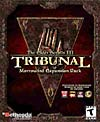
\includegraphics{media/image6.png}

ExplodeSpell ``spellName''

ExplodeSpell "proj\_trap\_spell"

The ExplodeSpell function makes a reference cast the given touch range
spell at itself. If an area effect touch range spell is used, this can
make the reference ``explode''. See the TrapProjScript, shown in the
tips and trick section on the Arrow trap.

\hypertarget{magic-getmodset-effects-functions}{%
\subsection{Magic Get/Mod/Set effects
functions:}\label{magic-getmodset-effects-functions}}

Most of these seem to refer to certain boni you normally get only from
spells. With these functions you can apparently make them permanent or
alter them. Most of these will normally use values between -100 to 100
(\%) but will accept any number, but others are flags (0 or 1). Thus,
you could make a creature that removes e.g. your ResistBlight bonus --
wouldn't that be a nice surprise for our Nerevarine?

\emph{Get/Mod/Set}ResistMagicka

\emph{Get/Mod/Set}ResistFire

\emph{Get/Mod/Set}ResistFrost

\emph{Get/Mod/Set}ResistShock

\emph{Get/Mod/Set}ResistDisease

\emph{Get/Mod/Set}ResistBlight

\emph{Get/Mod/Set}ResistCorprus

\emph{Get/Mod/Set}ResistPoison

\emph{Get/Mod/Set}ResistParalysis)

\emph{Get/Mod/Set}ResistNormalWeapons

\emph{Get/Mod/Set}WaterBreathing

Setting this to 1 enables water breathing

Get/Mod/SetChameleon

Corresponds to the Chameleon spell. This doesn't change the way the
player looks (as a spell cast would), but has the same effect otherwise,
i.e. NPCs may not detect the player and so on.

\emph{Get/Mod/Set}WaterWalking

Setting this to 1 enables water walking

\emph{Get/Mod/Set}SwimSpeed

\emph{Get/Mod/Set}SuperJump

These correspond to the Swift Swim and Jump spell effects, so they
normally range from 0 to 100, but work with negative or higher values as
well.

\emph{Get/Mod/Set}Flying

I found the following info on the UESP: This sets the player's flying
mode. To get this cheat to work, enter the console command and then cast
a Levitate Spell. The effect should now last until you disable the
flying with the console (thanks Dave Humphrey).

\emph{Get/Mod/Set}ArmorBonus

corresponds to shield effect

\emph{Get/Mod/Set}CastPenalty

corresponds to "Sound" effect? (<0 makes casting harder,
>0, easier)

\emph{Get/Mod/Set}Silence

\emph{Get/Mod/Set}Blindness

\emph{Get/Mod/Set}Paralysis

What it does is each paralysis effect you apply to the actor increments
the number by one. Each effect you remove decrements it by 1. You can
also alter these using the set and the mod functions. Whenever its zero
the actor can move. Try clicking on someone in the console and typing
setparalysis 1. What's good about it is if you have multiple actors of
the same ID, this allows you to paralyse an individual much like
targeting them with a spell would.\\
This is different from using a paralysis ability which would paralyse
all of that ID if you left the cell then went in again. Paralysing them
using SetParalysis lasts until you set it to zero or have gone out of
their cell for 3 days even if they are not autocalc npc's. (Forum info /
Cortex)

\emph{Get/Mod/Set}Invisibile

(Original MW: sic! Not invisible!)

\emph{Get/Mod/Set}Invisible

(Later versions of MW, apparently spelling was fixed at some point
(Forum info / Cortex))

\emph{Get/Mod/Set}AttackBonus

corresponds to fortify attack effect

\emph{Get/Mod/Set}DefendBonus

corresponds to sanctuary effect

\hypertarget{sound}{%
\section{\texorpdfstring{\hfill\break
Sound}{ Sound}}\label{sound}}

\hypertarget{make-actors-speak-an-audio-file}{%
\subsection{Make Actors speak an audio
file}\label{make-actors-speak-an-audio-file}}

Say, ``file name'', ``text''

Actor-> say,
"vo\textbackslash Misc\textbackslash CharGenBoat1.wav", "This is where
they want you."

Make subject "say" the sound file, only works on animating objects. The
.mp3 voice sound files can be found in "Data
files\textbackslash Sound\textbackslash Vo\textbackslash" folder and are
ordered in subfolders by race and gender. You can browse through most of
them in the dialogue/voice window as well. Text is what is displayed as
a subtitle as the file is played.

SayDone

Returns true if the calling object is not saying anything.

Sample Script: from character generation:

\lstinputlisting{scripts/CharGenBoatNPC.txt}

\hypertarget{playing-music}{%
\subsection{Playing music}\label{playing-music}}

{[}no fix{]} StreamMusic, ``filename.ext''

Plays the sound file "filename.ext", usually an mp3 file, as the current
music file. The music file should by default be located in the data
files/music/ folder. Stream music can also play MIDI files (JOG).

\textbf{Note:} Slightly bugged: Calling StreamMusic automatically sets
the music volume to 100, and leaves it there even after the music has
finished playing. Since there is no function to set the volume, the user
has to reset to his desired volume manually through the options menu.

\hypertarget{playing-sounds}{%
\subsection{Playing sounds}\label{playing-sounds}}

{[}no fix{]} PlaySound, ``sound ID''

{[}no fix{]} PlaySoundVP, ``sound ID'', volume\_enum, pitch\_enum

PlaySound3D, ``sound ID''

PlaySound3DVP, ``sound ID'', volume\_enum, pitch\_enum

"ex\_gg\_portcullis\_02"-> Playsound3DVP "Dwemer Door Open"
1.0 1.0

The PlaySound function plays a sound without any modification. It does
not matter to which object the script using the function is attached,
the sound will always play at full volume, directly in the player's ear,
so to speak.

The PlaySound3D function plays a directional sound source. The sound
will seem to be emitted by the object to which the script with this
function is attached.

The "VP" variants of each of these commands allow setting volume and
pitch for the sound that is played. Bethesda has not made much use of
this, it seems and it's only ever used with 1.0 set for both, which
appears to be the standard anyway. My own experiments showed the sound
not playing when I set volume to a variable, but this is no final
verdict.

The "sound ID" is the ID listed in the sound window accessed via
Gameplay -- sounds menu. You can add sounds there (place the .wav file
somewhere in Data files/sounds). A good source for sounds on the web is
%\url{http://www.findsounds.com/}.
Sounds should be in a certain format (see below) so you might have to change the format in a suitable program if you don't hear a sound in game.

\hypertarget{controlling-sound}{%
\subsubsection{Controlling sound}\label{controlling-sound}}

StopSound, "Sound ID"

Object\_ID-> StopSound "Lava Layer"

stops the sound "SoundID" if it is currently playing in the calling
object.

GetSoundPlaying, "sound ID" (returns Boolean/short)

if ( GetSoundPlaying "lava layer" == 0 )

Returns 1 when the specified sound is currently playing on the calling
object. The sound ID's can be found in the Gameplay menu /sounds and
/sound gen, where you can also set up your own (see below for formats).
This function can be used to control sounds, but also to gain
information, because certain sounds are tied to certain events in game,
e.g. the "Critical Damage" sound or the "Disarm trap" sound.

\textbf{Sample Script:} This simple script ensures that lava always has
its rumble sound playing:

\lstinputlisting{scripts/lava02.txt}

\hypertarget{sound-file-formats}{%
\subsubsection{Sound file formats}\label{sound-file-formats}}

\textbf{Note:} Not all sound files seem to play correctly in the game
(although all play in the editor). To be safe, use the formats used by
Bethesda (thanks to random name) :

"Cr" and the "Fx" folder\\
Windows PCM (.wav)\\
22050 kHz, 16-bit, Mono

Lower qualities work as well, e.g. 8,000 kHz; 8 Bit; Mono. Used e.g. in
my "The Regulars" mod for Tavern music.\\
\strut \\
"Vo" folder format\\
MPEG Layer-3, 64 Kbps\\
44100 kHz, 16-bit, Mono

\hypertarget{keeping-track-of-time}{%
\section{\texorpdfstring{\hfill\break
Keeping track of
time}{ Keeping track of time}}\label{keeping-track-of-time}}

There are a number of possibilities to follow the passage of time in
scripts, including some that are not, or only poorly documented in the
help file.

\hypertarget{timer}{%
\subsection{Timer}\label{timer}}

{[}no fix{]} GetSecondsPassed (returns float)

A simple timer can be scripted with the GetSecondsPassed function. It
returns the seconds passed \emph{since the last frame} as a float value.
To use this for a timer use something like the following example:

\lstinputlisting{scripts/TimerScript.txt}

{[}no fix{]} GetCurrentTime (returns float)

This returns the ingame time (24 hour) to two decimal places. This is
exactly the same as using the global GameHour variable, but slightly
less accurate.

\hypertarget{morrowinds-time-related-global-variables}{%
\subsection{Morrowind's time related global
variables}\label{morrowinds-time-related-global-variables}}

GameHour (is float global variable)

Day (is short global variable)

Month (is short global variable)

Year (is short global variable)

These globals get set by the game and contain the current date and time.

The MW calendar is a little bugged (thanks to samois for the info): MW
starts on Day 16, Month 7, Year 427. (16 Last seed)

The months are as follows, with the days in each month.

(Morning Star ???)

Suns Dawn 31

First Seed 28

Rain's Hand 31

Second Seed 30

Mid Year 31

Sun's Height 30

Last Seed 31

Heart Fire 31

Frost Fall 30

Suns Dusk 31

Evening Star 30

So there are 334 days in a MW year!?! Basically it seems that Bethesda
screwed up their code and lost a month, Morning Star / January\ldots{}
It seems the mistake was simply making it "wrap" to the wrong month from
Evening Star. If you manually set month to 0 it will correctly display
Morning Star in the rest menu. So this could be scripted around.

\textbf{Sample Script:} Checking the time of day with the GameHour
function:

\lstinputlisting{scripts/AfternoonTea.txt}

\hypertarget{keeping-track-of-days-passed}{%
\subsubsection{Keeping track of days
passed}\label{keeping-track-of-days-passed}}

Day (is short global variable)

Use the global ``Day'' variable. It contains the current "day of the
month" -- so on "17, last seed" it is 17. This can be used to keep track
of the number of days passed:

Short localdaysPassed

Short currentDay

if ( currentDay != Day ) ;whenever Day changes (presumably
increasing)\ldots{}

set currentDay to Day

set localdaysPassed to localdaysPassed + 1 ;add one to the counter

endif

This would usually be used for time-limited quests in a global script,
to make sure the passage of time is correctly measured. Innovative
scripting might also make use of it to trigger events after an item has
been in the player's possession for some time, etc.

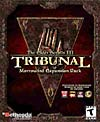
\includegraphics{media/image6.png}

DaysPassed (is short global variable)

Contains the number of days since the game started. In order to work,
DaysPassed has to be declared as a global short variable. This
declaration is present in Tribunal.esm, but not in Bloodmoon.esm. Thus,
in mods that make use of it, and that do not depend on Tribunal.esm,
DaysPassed MUST be declared explicitly. This may be one of the reasons
that some people reported it to be broken with Bloodmoon, but for others
it worked fine - it depends on whether they had Tribunal.esm checked or
not (Forum info / Erstam).

\hypertarget{moon-phases}{%
\subsubsection{Moon phases}\label{moon-phases}}

Indispensable for any potential werewolf mod.

{[}no fix{]} GetMasserPhase (returns short)

{[}no fix{]} GetSecundaPhase (returns short)

If (GetMasserPhase == 4)

{[}enable werewolf monster{]}

endif

\textbf{Note:} The helpfile lists \emph{GetSecundusPhase}, the above
syntax \emph{GetSecundaPhase} is the correct one. Also note that
GetMasserPhase and GetSecundaPhase return the value of the moon phases
for the last exterior cell you visited (Forum Info / Elim).

I only made a quick test with these, but they seem to work.

Both functions return short with these values:

0 =~MOON\_PHASE\_NEW (this is the default)

1 =~MOON\_PHASE\_WAXING\_CRESCENT or~MOON\_PHASE\_WANING\_CRESCENT:

2 =~MOON\_PHASE\_WAXING\_HALF or~MOON\_PHASE\_WANING\_HALF:

3 =~MOON\_PHASE\_WAXING\_GIBBOUS or~MOON\_PHASE\_WANING\_GIBBOUS:

4 =~MOON\_PHASE\_FULL

\hypertarget{weather}{%
\section{\texorpdfstring{\hfill\break
Weather}{ Weather}}\label{weather}}

\hypertarget{changing-weather}{%
\subsection{Changing weather}\label{changing-weather}}

{[}no fix{]} ChangeWeather, "RegionID", short\_Type\_Enum

ChangeWeather, "West Gash Region", 4

This function changes the weather in the indicated region to the weather
type specified by TypeEnum, and will change again to according to the
region settings after the time set by the game (I assume that is set in
the Morrowind.ini file in the Weather section. In mine the entry
reads:\\
Hours Between Weather Changes=20

The weather TypeEnum values are:

\begin{longtable}[]{@{}
  >{\raggedright\arraybackslash}p{(\columnwidth - 2\tabcolsep) * \real{0.35}}
  >{\raggedright\arraybackslash}p{(\columnwidth - 2\tabcolsep) * \real{0.65}}@{}}
\toprule
\endhead
0 & Clear \\
1 & Cloudy \\
2 & Foggy \\
3 & Overcast \\
4 & Rain \\
5 & Thunder \\
6 & Ash \\
7 & Blight \\
\bottomrule
\end{longtable}

\hypertarget{changing-weather-settings-for-a-region}{%
\subsection{Changing weather settings for a
region}\label{changing-weather-settings-for-a-region}}

{[}no fix{]} ModRegion, "RegionID", clear\_enum, {[}cloudy\_enum{]},
{[}foggy\_enum{]}, {[}overcast\_enum{]}, {[}rain\_enum{]},
{[}thunder\_enum{]}, {[}ash\_enum{]}, {[}blight\_enum{]},
{[}snow\_enum{]}, {[}blizzard\_enum{]}

ModRegion, "West Gash Region", 10, 20, 10, 5, 5, 40, 10, 0, 0, 0

Changes the weather chances for the RegionID. Used to get rid of, or add
weathers to an area permanently. The values must add up to 100 or you
will get odd results.

At least with Bloodmoon, all arguments except the first seem to be
optional. I am not sure if this remains true with Morrowind and
Tribunal.

If you want to maintain compatibility with a Morrowind only install, it
would be best to use only 8 arguments.

\hypertarget{determining-current-weather}{%
\subsection{Determining current
weather}\label{determining-current-weather}}

{[}no fix{]} GetCurrentWeather (returns short)

If ( GetCurrentWeather == 1 )

;{[}Do something if it is cloudy{]}

endif

This returns the weather TypeEnum listed above.

\textbf{Sample script:} Bethesda used this to make the banners move in
the wind according to weather type:

\lstinputlisting{scripts/OutsideBanner.txt}

\hypertarget{detecting-wind-speed}{%
\subsection{Detecting wind speed}\label{detecting-wind-speed}}

Undocumented:

{[}no fix{]} GetWindSpeed (returns float)

I have only very briefly tested this function and it returns values, 0
indoors and floats outdoors (varying quickly, in overcast weather the
values seemed to oscillate around 2). (Thanks to XPCagey for finding
this)

GetWindSpeed will return a value greater than 0 in interiors acting like
exteriors, which can be very useful if you need to detect an interior
acting like an exterior.

\textbf{Sample Script:} This script detects if the players current cell
is interior, exterior or interior acting like exterior.

if ( getInterior == 0 )

;outside

elseif ( getWindSpeed > 0.01 )

;Interior acting like exterior

else

;Interior

Endif

\hypertarget{player-sleeping}{%
\subsection{\texorpdfstring{\hfill\break
Player sleeping}{ Player sleeping}}\label{player-sleeping}}

{[}no fix{]} ShowRestMenu

Brings up rest menu, and allows the player to sleep. This is used e.g.
for beds in cells where it is otherwise illegal to sleep.

Sample Script: This is the standard script for beds:

\lstinputlisting{scripts/Bed_Standard.txt}

Returns true (1) if pc is sleeping. \textbf{Note:} The sleep selector
and counter you see while sleeping counts as a menu. So be aware of
that, if you want to use this function, and the MenuMode function in the
same script!

The \textbf{example script} seems to come from a fairly useless item,
but it demonstrates the use\ldots{}

\lstinputlisting{scripts/pillowScript.txt}

{[}no fix{]} WakeUpPC

Makes the PC wake up before the selected sleeping time is over.
Sometimes creates a monster if the player was sleeping outside. This
always happens if they try to sleep for only one hour, with longer times
it may or may not happen (Thanks to Manauser for this info). WakeUpPC
interrupts the rest only when you actually *sleep*. It does not affect
loitering in places where resting is forbidden (Forum info / Kir).

Sample script: This is an edited excerpt from the lengthy "sleepers"
script by Bethesda. It is responsible for giving you the dreams about
Dagoth Ur that plague the player during the main quest. It shows how
GetPCSleep and WakeUpPC can be used:

\textbf{if ( GetPCSleep == 0 )}

return

endif

Set dream to 0

if ( GetPCCell "Balmora" == 1 )

Set dream to 1

endif

if ( GetPCCell "Ald-ruhn" == 1 )

Set dream to 2

endif

{[}\ldots{]}

if ( dream == 0 )

Set doOnce to 0

;this makes sure you have to leave the city and come back for another
attack to occur

return

endif

AddTopic "Disturbing Dreams"

;add this topic, doesn't matter if you do it over and over

;THE FIRST DREAM...

if ( GetJournalIndex A1\_2\_AntabolisInformant >= 10 )

if ( GetJournalIndex A1\_Dreams < 1 )

\textbf{WakeUpPC}

MessageBox "You had a disturbing dream. Bla bla bla", "Ok"

Journal A1\_Dreams 1

return

endif

endif

\hypertarget{enabling-and-disabling-player-control-and-interface}{%
\subsection{Enabling and disabling player control and
interface}\label{enabling-and-disabling-player-control-and-interface}}

\hypertarget{disable-player-control-functions}{%
\subsubsection{Disable player control
functions}\label{disable-player-control-functions}}

All of these functions disable some part of the user interface, thus
restricting the players actions.

{[}no fix{]} DisablePlayerControls

Player can only look around with mouse or use options menu, nothing else
and menus disappear.

{[}no fix{]} DisablePlayerFighting

{[}no fix{]} DisablePlayerMagic

These two functions seem to be unreliable according to forum
information: If the player holds a weapon or has a spell readied he can
continue to use it and quick-keys for weapons and spell likewise still
seem to work. I currently don't know of a reliable solution for this
problem.

{[}no fix{]} DisablePlayerJumping

{[}no fix{]} DisablePlayerLooking

{[}no fix{]} DisablePlayerViewSwitch

{[}no fix{]} DisableVanityMode

\hypertarget{enable-player-control-functions}{%
\subsubsection{Enable player control
functions}\label{enable-player-control-functions}}

Once a disable function has been used, the corresponding enable function
can be used to restore control.

{[}no fix{]} EnableLevelUpMenu

{[}no fix{]} EnablePlayerControls (Enables the controls and menus.)

{[}no fix{]} EnablePlayerJumping

{[}no fix{]} EnablePlayerFighting

{[}no fix{]} EnablePlayerLooking

{[}no fix{]} EnablePlayerMagic

{[}no fix{]} EnablePlayerViewSwitch

{[}no fix{]} EnableRest

{[}no fix{]} EnableVanityMode

\hypertarget{check-player-control-status}{%
\subsubsection{Check player control
status}\label{check-player-control-status}}

All of these functions return 1 if the corresponding "Disable" function
has been called and is active, 0 if control is with the player.

{[}no fix{]} GetPlayerControlsDisabled

{[}no fix{]} GetPlayerFightingDisabled

{[}no fix{]} GetPlayerJumpingDisabled

{[}no fix{]} GetPlayerMagicDisabled

{[}no fix{]} GetPlayerLookingDisabled

GetPlayerViewSwitch

(\textbf{Broken}, function does not work. Instead use: )

{[}no fix{]} GetVanityModeDisabled

\hypertarget{force-first-or-third-person-view}{%
\subsubsection{Force first or third person
view}\label{force-first-or-third-person-view}}

{[}no fix{]} PCGet3rdPerson (returns Boolean/short)

returns 1 if in 3\textsuperscript{rd} person mode

{[}no fix{]} PCForce3rdPerson

queue the change to 3\textsuperscript{rd} person mode (this may have to
wait for the animation to finish)

{[}no fix{]} PCForce1stPerson

same as above but 1\textsuperscript{st} person mode

(See also the console command "ToggleVanityMode" (TVM).

\hypertarget{functions-for-character-generation-menus}{%
\subsubsection{Functions for character generation
menus}\label{functions-for-character-generation-menus}}

These undocumented functions are used for character creation. They
enable all the menus that are used during the character creation process
and enable certain basic features like the inventory, magic menu, stats
window and the map:

Show character generation menus:

{[}no fix{]} EnableBirthMenu\\
{[}no fix{]} EnableClassMenu\\
{[}no fix{]} EnableRaceMenu\\
{[}no fix{]} EnableNameMenu

There is no disable command for these. They are disabled by selecting ok
in the menu.

Enabling in-game menus:

{[}no fix{]} EnableMagicMenu\\
{[}no fix{]} EnableMapMenu\\
{[}no fix{]} EnableInventoryMenu\\
{[}no fix{]} EnableStatsMenu

Also no disable commands here unfortunately. These would have been
useful.

The names of the functions should be self-explanatory. One use for these
functions is as a cheat if you want to change your appearance or other
things during a running game (although there might be problems
associated with doing that). They can (and have been) used to create
different ways of character generation. Be careful, sometimes these
reset your level to 1.

\textbf{Sample Script:} This is one of many CharGen scripts that guide
the player through character generation. This one is basically a safety
feature for a player who just runs out the door, without triggering any
or all of the little tutorials.

\lstinputlisting{scripts/CharGenDoorExit.txt}

\hypertarget{determining-if-player-has-menus-open}{%
\subsection{Determining if player has menus
open}\label{determining-if-player-has-menus-open}}

{[}no fix{]} MenuMode

If ( MenuMode == 1 )

MenuMode returns one if the player has menus open, and 0 otherwise.
\textbf{This doesn't only apply to the inventory and dialogue menus.}

A good explanation is given by DinkumThinkum:

\emph{It looks to me as though the game considers 'MenuMode' to be
anytime the mouse pointer is on the screen instead of the crosshairs.
I.e., any time you can move the mouse pointer around on the screen to
select things, rather than the whole display moving and you can only
select items at the center of the screen.\\
\strut \\
For example, hitting Escape for the in-game Options menu, displaying a
message box with an "OK" button (or any other clickable buttons),
hitting '`' for the console window: all those count as menu mode, in
addition to the more obvious ones such as the dialogue window, the
character data/map/inventory screen, the container window, etc.}

It is common practice to put the following lines at the beginning of
almost any script, to prevent unnecessary or problematic functions being
processed in MenuMode:

If ( MenuMode == 1 )

Return

Endif

\hypertarget{using-menutest-to-open-and-close-menus}{%
\subsection{Using MenuTest to open and close
menus}\label{using-menutest-to-open-and-close-menus}}

Undocumented:

{[}no fix{]} MenuTest, short\_enum

MenuTest doesn't return anything, however, when it is called, it closes
certain types of inventory menus, including Player, NPC and containers.
It doesn't work for dialogue, enchanting, alchemy, spell or armorer
menus. (Forum Info / JOG, Jilin).

menutest or menutest 0 for closing menu

menutest 3 open stats menu or focus on it

menutest 4 open inventory menu or focus on it

menutest 5 open spell menu or focus on it

menutest 6 open map menu or focus on it

for menutest 3,4,5,6, it's like clicking on the upper right button of
the menu

Example Script:

if ( OnPCEquip == 1 )

set OnPCEquip to 0

coc Balmora

\textbf{MenuTest}

endif

\hypertarget{miscellaneous-functions-and-variables}{%
\section{\texorpdfstring{\hfill\break
Miscellaneous functions and
variables}{ Miscellaneous functions and variables}}\label{miscellaneous-functions-and-variables}}

\hypertarget{breaking-of-script-processing}{%
\subsection{Breaking of script
processing}\label{breaking-of-script-processing}}

{[}no fix{]} Return

Return tells the game engine to finish processing the script for this
frame. All code below this line will be ignored for this frame. In the
next frame the script is executed again \textbf{from the top}.

If ( MenuMode == 1 )

Return

Endif

Careful: Anything below a return function will not be processed, even if
there are "true" if statements there! So use this with caution.

\hypertarget{controlling-global-scripts}{%
\subsection{Controlling global
scripts}\label{controlling-global-scripts}}

These function are used to control global scripts. Global scripts have
to be started with the StartScript function (either from another local
or global script or from a dialogue result field) and a running script
can be terminated with the StopScript function.

Tribunal "Start Scripts" in a plug-in start executing each time the game
is loaded. If a Tribunal Start Script is terminated with a 'StopScript',
it will start up again the next time the game is loaded - see the Tip
and Tricks section on "Detecting when a player does a load from
savegame". (Forum info / DinkumThinkum).

To my knowledge these functions do not work with local scripts attached
to objects, you can however start and stop "targeted scripts" by using
an object "fix": "ObjectID-> StartScript" (for more info see
the Tips and Tricks section on targeted scripts).

StartScript, "ScriptName"

This starts the specified script.

\textbf{Warning:} When you use startscript, all the scripts that have
been run before you called startscript will be re-run, so scripts could
be run more than once in the same frame.

{[}no fix?{]} ScriptRunning, "ScriptName" (returns Boolean/short)

The ScriptRunning function returns 1 if a script is running, 0 if it's
not running:

if ( ScriptRunning, CharGen == 0 )

StartScript CharGen

Endif

StopScript, "ScriptName"

Stops the specified script

\textbf{Note:} If you use 'StopScript' from inside the global script
you're terminating, it doesn't actually terminate the script
immediately. Instead, the script continues executing to the 'End'
statement, and then terminates. So you still need to use "Return" if you
don't want the rest of the script to be processed.

StopScript can also be used to construct do-once conditions for global
scripts in a very clean way by self-terminating the script:

\lstinputlisting{scripts/do-once_script.txt}

\hypertarget{fading-the-screen-in-and-out}{%
\subsection{Fading the screen in and
out}\label{fading-the-screen-in-and-out}}

{[}no fix{]} FadeIn time\_float\_enum

{[}no fix{]} FadeOut time\_float\_enum

{[}no fix{]} FadeTo alpha\_enum time\_float\_enum

FadeTo 50 2.0 ;(Fades screen to 50\% in 2 seconds)

FadeIn and Fadeout fades the screen (not an object) to blackness in the
time specified (in seconds). Time is > 0 and <=
10.0. FadeTo fades only to a certain percentage: 0 is full transparency.
100 is black.

\hypertarget{adding-a-location-to-the-map}{%
\subsection{Adding a location to the
map}\label{adding-a-location-to-the-map}}

{[}no fix{]} ShowMap "cell ID"

ShowMap "Gnisis"

This function will highlight the indicated cells. Cell ID can be full or
partial, i.e. all cells that begin with the given string will be
highlighted on the world map (e.g. ShowMap "Vivec" will highlight all
the cantons).

\textbf{Sample Script:} reading this book will indicate all these places
on the world map:

\lstinputlisting{scripts/bookPilgrimsPath.txt}

Also see "FillMap" console command.

\hypertarget{assigning-random-values-to-variables}{%
\subsection{Assigning random values to variables}\label{assigning-random-values-to-variables}}

{[}no fix{]} Random, value\_enum

Set my\_variable to Random, 50

Introducing some unpredictability into the effects of a script is a nice
option, and it can be done with the \emph{Random} function.
\emph{Random} returns values between 0 and the set value --1. So in the
example above, my\_variable will be set to a value in the range from 0
to 49.

Note that the global short variable Random100 gets set each frame by the
game's \emph{Main} script to a random value between 0 and 100
(inclusive), so you can make use of that one, too.

Note that if you are using random100 in dialogue, you may want to add:

set random100 to random, 101

in the resultbox so that random100 is reset for the next topic chosen.
Main does not set random100 in menumode.

\textbf{Note}: For any call to Random with a range over 100, the
randomosity of the return value gets very poor indeed... right up to
Random, 255 where you only get 0 or 1... and any multiple of 256 also
gets you a CTD. (Morrowind and Tribunal). In Bloodmoon, they seem to
have fixed the randomosity of the return value... you seem to get
numbers that are more evenly distributed, even with a range above 100.
But the CTD's at 256 and 512, etc, still happen (Info by Neko). It was
furthermore discovered that sometimes the Random cap is set much higher
than the number given. Setting any variable to a Random with the cap
value of one of the following numbers produces some strange result,
setting the higher cap actually to something around 1100: 65, 66, 68,
70, 71, 76, 77, 79, 82, 83, 84

TunaandCheese suggests that a method to work arround the poor
randomosity in Morrowind and Tribunal is to merge Random results, as is
demonstrated in this script:

\textbf{begin randomnumber}

\textbf{;this script works out a random number between 0 and 10000\\
\strut \\
short spare\\
short number\\
}

\textbf{;works out how many thousands there are\\
set number to random, 10\\
set number to ( number * 1000 )\\
}

\textbf{;how many hundrerds\\
set spare to random, 10\\
set spare to ( spare * 100 )\\
set number to ( number + spare )\\
}

\textbf{;and how many tens\\
set spare to random, 10\\
set spare to ( spare * 10 )\\
set number to ( number + spare )\\
}

\textbf{;this has to be random, 11, rather than random, 10 as if it was
random 10,}

\textbf{;it would only be 0 - 9999\\
set spare to random, 11\\
set number to ( number + spare )}

\textbf{;the variable number now contains a random number between 0 and
10,000 that you can use\\
\strut \\
end}

\hypertarget{playing-videos}{%
\subsection{Playing videos}\label{playing-videos}}

{[}no fix{]} PlayBink ``filename'' flag\_enum

Pauses game and plays video. Set Flag to true if player can escape
movie.

The video needs to be in Bink format and placed into the
Datafiles/Videos directory.

To convert a video to Bink format you need to use
\href{http://www.radgametools.com/bnkdown.htm}{The RAD Video Tools}.

\hypertarget{levelled-list-functions}{%
\subsection{Levelled List functions}\label{levelled-list-functions}}

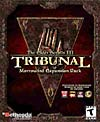
\includegraphics{media/image6.png}

{[}no fix{]} AddToLevCreature ``levcreaname'' ``creature\_ID''
level\_enum

{[}no fix{]} AddToLevItem ``levitemname'' ``item\_Id'' level\_enum

{[}no fix{]} RemoveFromLevCreature ``levcreaname'' ``creature\_ID''
level\_enum

{[}no fix{]} RemoveFromLevItem ``levitemname'' ``item\_ID'' level\_enum

These functions are used to manipulate Leveled Item and Leveled Creature
lists at run-time. Leveled lists are comprised of object/level pairs
where the level is the level the PC has to be to encounter the object.
The AddTo functions will add the given object/level pair to the
specified leveled list as long as the list does not already contain a
matching pair. The RemoveFrom functions will remove all occurrences of
the object/pair from the leveled list. \textbf{Additionally, if a
RemoveFrom function is given an object pair with a level of --1, all
object pairs containing the specified object are removed.}

\textbf{Note:} The RemoveFrom functions will not remove existing objects
from the world. If a Leveled Creature reference has already calculated
to be a certain creature, removing that creature from the Leveled
Creature's list will not get rid of the existing creature in the world.
However it will prevent that Leveled Creature reference from calculating
to be that creature again.

\textbf{Note:} The ability of creature leveled lists to call other
leveled lists is \textbf{only} in Bloodmoon. Those wishing to "nest"
creature leveled lists in their plugins must have that Bloodmoon
dependency, even if they use no objects from Bloodmoon. (forum info /
blockhead)

\textbf{Warning:} It is not recommended that you use these functions as
it will break any other mod that uses leveled lists.

DarkDragon writes on the Official forums:\\
\emph{The problem lies in the way Morrowind loads items. First it loads
ESMs, then ESPs, which can modify the leveled lists. If you have a list
merger, you can merge those lists and keep the changes from all of them
(where as before, the last loaded mod would take precedence). Then it
loads ESS, or save files.}

\emph{\hfill\break
The problem is, if a script adds something to a Leveled List, it
modifies the ESS (save game) and the save game then has a reference to
that Leveled list. This is loaded last and it overwrites ANY changes
done by other mods.}

Sample Script:

When this script is placed on an object, activating it will toggle the
existence of rats in the world by removing them from a Leveled Creature
and removing rat meat from a Leveled Item.

\lstinputlisting{scripts/norats.txt}

\hypertarget{square-root}{%
\subsection{Square root}\label{square-root}}

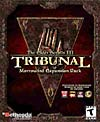
\includegraphics{media/image6.png}

{[}no fix{]} GetSquareRoot, number (float)

set var\_1 to GetSquareRoot var\_2

The GetSquareRoot function returns the square root of the given number.
This can be useful for vector or distance calculations (remember
Pythagoras?).

It is possible to get the square root of a number without using this
function, however it is significantly slower. See Soralis's Math mod for
an example script. MWSE also has a square root function.

\hypertarget{water-level-functions}{%
\subsection{Water Level Functions}\label{water-level-functions}}

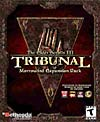
\includegraphics{media/image6.png}

{[}no fix{]} GetWaterLevel (float)

{[}no fix{]} SetWaterLevel newWaterLevel\_float

{[}no fix{]} ModWaterLevel waterLevelChange\_float

A great opportunity for cruel traps\ldots{} These functions are used to
determine and modify the Water Level of the current interior cell. When
an Actor suddenly finds itself underwater, it will wait until it is
halfway out of breath and then begin to make its way to the surface in a
straight line up. Floating corpses are moved with the water without
regard for collision.

\textbf{Note:} If you use GetWaterLevel in a interior cell with no
water, GetWaterLevel will still return a result other than 0.

\textbf{Note:} Set/ModWaterLevel doesn't work in exteriors.

Sample scripts:

This script goes on a crank to make it raise or lower the water level in
the room.

\lstinputlisting{scripts/crank.txt}

This modified ``Float'' script is placed on any object with a centered
pivot point to make it float on the water's surface regardless of water
level. It also will make the object stop bobbing if the PC is standing
on it.

\lstinputlisting{scripts/NewFloat.txt}